\documentclass{mimosis}
\usepackage{scrhack}

\usepackage{metalogo}

%%%%%%%%%%%%%%%%%%%%%%%%%%%%%%%%%%%%%%%%%%%%%%%%%%%%%%%%%%%%%%%%%%%%%%%%
% Some of my favourite personal adjustments
%%%%%%%%%%%%%%%%%%%%%%%%%%%%%%%%%%%%%%%%%%%%%%%%%%%%%%%%%%%%%%%%%%%%%%%%
%
% These are the adjustments that I consider necessary for typesetting
% a nice thesis. However, they are *not* included in the template, as
% I do not want to force you to use them.

% This ensures that I am able to typeset bold font in table while still aligning the numbers
% correctly.
\usepackage{etoolbox}


\usepackage[binary-units=true]{siunitx}
\DeclareSIUnit\px{px}

\sisetup{%
  detect-all           = true,
  detect-family        = true,
  detect-mode          = true,
  detect-shape         = true,
  detect-weight        = true,
  detect-inline-weight = math,
}

%%%%%%%%%%%%%%%%%%%%%%%%%%%%%%%%%%%%%%%%%%%%%%%%%%%%%%%%%%%%%%%%%%%%%%%%
% Hyperlinks & bookmarks
%%%%%%%%%%%%%%%%%%%%%%%%%%%%%%%%%%%%%%%%%%%%%%%%%%%%%%%%%%%%%%%%%%%%%%%%

\usepackage[%
  colorlinks = true,
  citecolor  = RoyalBlue,
  linkcolor  = RoyalBlue,
  urlcolor   = RoyalBlue,
  unicode,
  ]{hyperref}

\usepackage{bookmark}

%%%%%%%%%%%%%%%%%%%%%%%%%%%%%%%%%%%%%%%%%%%%%%%%%%%%%%%%%%%%%%%%%%%%%%%%
% Bibliography
%%%%%%%%%%%%%%%%%%%%%%%%%%%%%%%%%%%%%%%%%%%%%%%%%%%%%%%%%%%%%%%%%%%%%%%%
%
% I like the bibliography to be extremely plain, showing only a numeric
% identifier and citing everything in simple brackets. The first names,
% if present, will be initialized. DOIs and URLs will be preserved.

\usepackage[%
  autocite     = plain,
  backend      = biber,
  doi          = true,
  url          = true,
  giveninits   = true,
  hyperref     = true,
  maxbibnames  = 99,
  maxcitenames = 99,
  sortcites    = true,
  style        = numeric,
  ]{biblatex}

\input{Bibliography/bibliography-mimosis}
\addbibresource{Bibliography/thesis.bib}

%%%%%%%%%%%%%%%%%%%%%%%%%%%%%%%%%%%%%%%%%%%%%%%%%%%%%%%%%%%%%%%%%%%%%%%%
% Fonts
%%%%%%%%%%%%%%%%%%%%%%%%%%%%%%%%%%%%%%%%%%%%%%%%%%%%%%%%%%%%%%%%%%%%%%%%

\ifxetexorluatex
  \setmainfont{Minion Pro}
\else
  \usepackage[lf]{ebgaramond}
  \usepackage[oldstyle,scale=0.7]{sourcecodepro}
  \singlespacing
\fi

\renewcommand{\th}{\textsuperscript{\textup{th}}\xspace}

\makeindex
\makeglossaries  % loading glossary from the glossary-directory
\loadglsentries{Gloss_Acr/glossary}

%%%%%%%%%%%%%%%%%%%%%%%%%%%%%%%%%%%%%%%%%%%%%%%%%%%%%%%%%%%%%%%%%%%%%%%%
% Incipit
%%%%%%%%%%%%%%%%%%%%%%%%%%%%%%%%%%%%%%%%%%%%%%%%%%%%%%%%%%%%%%%%%%%%%%%%

%\title{\texttt{latex-mimosis}}
\title{Konzeption und Entwicklung eines\\ datengetriebenen Unterstützungssystems\\ für
Etatplanung und Mittelallokation\\ einer hybriden
Spezialbibliothek}
\author{Peter Breternitz}


\begin{document}


\frontmatter

  \includepdf{kruscht/pebr1698_2121_cover.pdf}
  \begin{titlepage}
    \vspace*{5cm}
    \makeatletter
    \begin{center}
      \begin{Large}
        \@title
      \end{Large}\\[0.1cm]
      %
      %\begin{Large}
        %\@subtitle
      %\end{Large}\\
      %
      \emph{von}\\
      \@author
      %
      %\vfill
      %Masterarbeit zur Erlangung des 
      %akademischen Grades\\
      %\emph{Master}\\
      %an der \\
      %\textsc{Technischen Hochschule Wildau}
    \end{center}
    \vspace{7.5 cm}
     Betreuer:\\ 
      \hspace*{1.5cm} Dipl.-Inf. Sascha Szott\\
      \hspace*{1.5cm} Dr. Frank Seeliger
    \makeatother
  \end{titlepage}
  
  \newpage
  \null
  \thispagestyle{empty}
  \newpage
  \begin{center}
    \textsc{Abstract}
  \end{center}
  %
  \noindent
  %
  Due to economic developments, libraries have to use their budgets efficiently and in line with its needs. 
  In addition, negotiations about the budgets in libraries are becoming increasingly important. 
  The goal of this master's thesis, was to design and develop a proof-of-concept of a data-driven support system 
  that enables the library of the Max Planck Institute for Empirical Aesthetics to use and plan its budget more efficiently.
  For this purpose, data from different library areas were analyzed and evaluated. 
  The data-driven support system shows essential key performance indicators such as budget, 
  expenditures, circulation, collection development, and reading room usage in a single dashboard. 
  This lays the foundation for the library to plan its budget and allocate resources more efficiently and in line with its needs.

  

\begin{center}
    \textsc{Zusammenfassung}
  \end{center}

  \noindent
  %
Aufgrund von ökonomischen Entwicklungen müssen Bibliotheken ihre Budgets effizient und bedarfsgerecht einsetzen. 
Zudem werden Verhandlungen über die Budgets in Bibliotheken immer wichtiger. 
Das Ziel der vorliegenden Masterarbeit, war es ein Proof-of-Concept eines datengetriebenen Unterstützungssystems 
zu konzipieren und zu entwickeln, dass die Bibliothek des Max-Planck-Institutes für empirische Ästhetik in die Lage versetzt,
ihr Budget effizienter zu planen und einzusetzten. Dafür wurden aus verschiedenen bibliothekarischen Bereichen Daten analysiert 
und ausgewertet. Das datengetriebene Unterstützungssystem ermöglicht wesentliche Key Performance Indicators wie Budget, 
Umsatz, Ausleihe, Bestandsentwicklung sowie die Lesesaalnutzung in einem Dashboard anzuzeigen. 
Damit ist ein Grundstein für die Bibliothek gelegt, die Planung des Budgets und der Einsatz Mittelallokation effizienter
und bedarfsgerechter zu gestalten.
  %\lipsum[1]


  \tableofcontents


  

\mainmatter

  \chapter{Einführung}
\section{Problemstellung}
\section{Ziel der Arbeit}
\section{Verwandte Arbeiten}
\section{Gliederung der Arbeit}


  %\chapter{Einführung}
Als Ende des Jahres 2019 der Ausbuch der Covid-19-Pandemie begann, entwickelte die 
Johns Hopkins University zu Beginn des darauf folgenden Jahres ein Dashboard als Antwort
auf den anhaltetenden Notstand im Bereich der öffentlichen Gesundheit. Diese visualisiert seit je
die gemeldeten Fälle weltweit. Es wurde entwickelt, um Forschern, Gesundheitsbehörden und der breiten Öffentlichkeit 
ein benutzerfreundliches Instrument an die Hand zu geben, mit dem sich der Ausbruch verfolgen lässt. 
Zu dessen Datenquellen gehören unter anderem die Informationen der Weltgesundheitsorganisation, staatliche und nationale
Gesundheitsämter. Diese  wurden aggregiert und verdichtet. So visualisiert das Dashboard mit einer Landkarte und Punkten den Ausbruch. 
Dazu gibt es Zahlen der bestätigten COVID-19-Fälle, Todesfälle und Genesungen für alle betroffenen Länder.
Das faszinierende an dem Dashboard ist, das es gelungen ist, alle relevanten Zahlen auf einer Seite darzustellen
und somit der interessierten Öffentlichkeit schnell einen Überblick zu verschaffen.

\section{Problemstellung}
%Das große Problem\\
Ausgehend von ökonomischen, informationstechnologischen und marktpolitischen Einschnitten in den
vergangenen Jahrzehnten \footnote{Als Gründe zu nennen wären hier: die Explosion der Zeitschriftenpreise im Bereich der
Science, Technology \& Medicine (STM), das Aufkommen von E-Publishing und die Konzentration auf wenige
Verlage},sind Bibliotheken dazu veranlasst, ihr Budget hinsichtlich der Informationsbedarfe
ihrer Nutzer:innen behutsamer zu planen und sich in zunehmenden Maße gegenüber ihren Unterhaltsträgern zu rechtfertigen.
Die Relevanz von bibliothekarischen Kennzahlen ist in diesem Zusammenhang größer geworden.
Deswegen ist es wichtig, Daten aus bibliothekarischen Servicedienstleistungen und Geschäfts-prozessen zu aggregieren, zu erheben und statistisch
auszuwerten, um auf Basis der daraus erzielten Erkenntnisse handeln zu können.

%Was ist der Markt?\\
%--------------------
Es gibt eine Vielzahl kommerzieller Lösungen für den Bibliotheksbereich, die auf Business-Intelligence-Systemen basieren.
Zu nennen wären \textit{AlmaAnalytics} für das Next-Generation-Library-System \textit{Alma} von \textit{ExLibris}\footnote{\url{https://www.exlibrisgroup.com/products/alma-library-services-platform/alma-analytics}
Stand: 26.05.2020}, \textit{BibControl} von \textit{OCLC}\footnote{\url{https://www.oclc.org/de/bibcontrol.html} Stand: 26.05.2020},
\textit{CollectionHq} von \textit{Baker \& Taylor}\footnote{\url{https://www.collectionhq.com/} Stand: 26.05.2020} oder \textit{Libinsight} von \textit{SpringShare}\footnote{\url{https://springshare.com/libinsight/} Stand: 26.05.2020}.
Darüber hinaus gibt es Business-Intelligence-Applikationen, die von Bibliotheken für Reporting, Datenanalyse und Datenvisualisierung adaptiert werden,
wie zum Beispiel \textit{Tableau} von der Firma \textit{Tableau Software} oder
\textit{Crystal Reports} von \textit{SAP}.
Diese Applikationen sind entweder an bestimmte Bibliothekssysteme zurückgebunden, limitiert in ihren
Funktionen\cite{golas_statistische_2018} oder zu generisch.
%Überdies wird sowohl von \textit{HeBis} bzw. von der
%Lokal-Bibliothekssystembetreuung als auch von der \textit{mpdl} keine Applikation
%in dieser Richtung angeboten.
%Ebenso ist ungewiss, wann die Ablösung des schon betagten \textit{CBS/LBS} hin zu
%einem neuen Next-Generation-Library-System im \textit{HeBis-Verbund} stattfinden wird und ob
%es ein Modul zur statistischen Datenerhebung liefern wird.

%Wem hilft es?\\
%--------------
Die Notwendigkeit für diese Applikation ist durch das
Fehlen eines zentralen Nachweisortes für bibliothekarische
Statistiken in der Bibliothek gegeben. Da die Bibliothek zudem verschiedene Recherche-Systeme den
Wissenschaftler:innen anbietet, wäre eine Engführung der statistischen
Datenerhebung auf eine Plattform begrüßenswert.
Des Weiteren ist das Erfordernis, bibliothekarische Geschäftsprozesse zu evaluieren und die
Servicedienstleistungen bezüglich der Ziele der Institution noch weiter zu
optimieren, von großer Relevanz. 
Die zu entstehende Applikation könnte hierbei helfen, systematisches Controlling einzuführen und das
Bibliotheksmanagement weiter zu professionalisieren.
%predictive analysis\\
Um künftigen Anforderungen gewachsen zu sein, soll sie
modulbasiert programmiert werden und dadurch leicht erweiterbar und eventuell von
anderen Bibliotheken nachnutzbar sein.
f
%Warum jetzt?\\
%--------------

Mit dem Ende der Konsolidierungsphase der
Bibliothek, die im Zuge des \textit{Max-Planck-Institutes für empirische
Ästhetik} 2014 gegründet wurde, tritt sie ein in eine Phase, in der ab dem Jahr
2021 Budgetplanungen eine größere Rolle spielen werden.

Ist das Problem lösbarerer geworden?\\
-------------------

Wodurch?\\
--------------------


Was ist der Trend?\\
---------------------
Dashboards in aller Munde


\section{Ziel der Arbeit}

Was ist Ihr relevantes Teilproblem? Was ist Ihre zentrale Frage?\\
Ihr Ziel der Arbeit in zwei Sätzen.\\
Warum genau dieses Problem?\\
Ist Ihr Beitrag völlig neu, oder nur ein Baustein?\\
Ist Ihr Problem schwer zu lösen oder „straight forward“?\\
Eher Forschung oder eher Anwendung?\\

Wenn Sie ein System bauen...\\
Welche Anfragen / Aufgaben wollen Sie beantworten / lösen können?\\
Welche Kernfunktionalität soll Ihr System haben?\\
Was ist ein typischer (Bedienungs-) Prozess für Ihr System? Wer nutzt Ihr System, Ihren Algorithmus? Wodurch ist dieses Nutzungsverhalten gekennzeichnet?\\

Anleihen von BI-Systemen in der Architektur

Schaffung eines Dashboards für Budgetplanung in Bibliotheken Ziel der zu entstehenden Arbeit ist die Entwicklung einer interaktiven Business-Intelligence-Applikation als proof-of-concept,
mit der systematisch die relevanten Daten einer hybriden Spezialbibliothek aggregiert, statistisch
analysiert und mit geeigneten und modernen Datenvisualisierungstechniken\footnote{Visualisierungen können komplexe Sachverhalte herunterbrechen und
so große Datenmengen - im Gegensatz zu großen Tabellen - leicht verständlich
darstellen. Im Kontext dieser Arbeit konzentriere ich mich auf Ansätze, die Visualisierungen mittels Visualisierungstechniken algorithmisch aus
Daten erzeugen (Informationsvisualisierung, Datenvisualisierung und visuelle Analyse).\cite{mayank_yuvaraj_infographics_2017}}
ausgegeben werden sollen.
Vor allem soll sich hier auf automatisierte Prozesse zur Gewinnung der Ergebnisse konzentriert werden.

Mit diesen automatisch angefertigten statistischen Datenanalysen sollen zukünftige
Entscheidungen im Bibliotheksmanagement wie Erwerbungspolitik, Budgetplanung und
Mittelallokation hinsichtlich der weiteren Entwicklung der
Servicedienstleistungen evidenzbasiert und datengetrieben unterstützt werden.

Darüber hinaus soll die Applikation  eine Funktion beinhalten, ausgewählte
Resultate automatisiert als \textit{factsheet} zu exportieren, um diese
als Rechenschaftsbericht gegenüber Stakeholdern der Bibliothek präsentieren zu können.

\section{Verwandte Arbeiten}

% Welche Vorarbeiten gibt es schon?\\
% Wo und Wann sind die Vorarbeiten entstanden?\\
% Welche Ziele haben die Vorarbeiten verfolgt?\\
% Auf welche Schwierigkeiten sind sie gestossen?

Ein gutes Beispiel für ein datengetriebenes Unterstützungssystem findet sich in
der Literatur bei Spielberg, der sich mit dem Thema der Bestandspflege an der
\textit{Universitätsbibliothek Essen} befasst und eine Applikation (weiter-)entwickelt hat, die
die Fachreferent:innen bei der Aussonderung und Erwerbung von Medien
unterstützt.\cite{spielberg_eike_t_fachref-assistent_nodate}
Ebenso finden sich in der Fachliteratur Ansätze, die vorrangig anhand einzelner
Fragestellungen hinsichtlich der Bestandsentwicklung\cite{hughes_long-term_2016} oder anderer
bibliothekarischer Servicedienstleistungen\cite{kutlay_shiny_2020, knievel_use_2006,meyer_using_2018} verschiedene statistische Analysen
vollzogen und diese visualisiert haben.
Eine Ausnahme bildet die Entwicklung eines Dashboards an der \textit{New York
University Health Sciences Libraries}, das versucht, möglichst viele Metriken
aus bibliothekarischen Dienstleistungen aufzunehmen.\cite{morton-owens_trends_2012}
Fast alle Projekte sind an größeren
Universitätsbibliotheken mit ganz unterschiedlichen softwaretechnischen
Herangehensweisen\cite{finch_using_2016, wiegand_visualizing_2013} und Zielen\cite{phetteplace_effectively_2012} entstanden.

Dennoch fehlen in der gesichteten Literatur Teile, die sich mit der Budgetierung
befassen und Auskunft über Mittelallokation geben.

Zudem fehlt ein Beispiel in der Literatur, das holistisch alle relevanten Daten, die in den
Geschäftsgängen und Servicedienstleistungen insbesondere einer Spezialbibliothek entstehen,
aggregiert, auf diesen Daten automatisch statistische Analysen ausführt und diese mit modernen Visualisierungstechniken
interaktiv darstellt.

Anwendung kommen deskriptive Statistik, es geht vielmehr darum Daten zusammen zu tragen, als diese zu explorieren 
Abgrenzung deskriptive Statistik / explorative Datenanalyse

\section{Gliederung der Arbeit}
%Wann lesen wir was und warum?\\
Im \autoref{chap:two} werden die theoretischen Grundlagen für die folgenden Kapitel gelegt. Das Kapitel befasst
sich mit den Themen Bibliothek und Statistik, Datenvisualisierung und Business-Intelligence-Systemen. Im \autoref{chap:three}
wird die Bibliothek vorgestellt und darauf eingegangen welche bibliothekarischen Statistiken bereits erhoben wurden.
Nachdem die Ausgangssituation bestimmt wurde, wird mit der Anforderungsanalyse im \autoref{chap:four} die Konzeption einer Lösung vorgestellt.
Im \autoref{chap:five} wird die Umsetzung diskutiert. Bevor das System bewertet wird, wird das Design und die Implementierung vorgestellt.
Das Fazit wird im \autoref{chap:six} mit dem Stand der Umsetzung, den lessons learned und einem Ausblick auf Themen, die noch bearbeitet werden könnten, gezogen.

  \chapter{Theoretische Grundlagen}
\label{chap:two}
In diesem Kapitel wird der theoretische Rahmen für die weiteren Kapitel gelegt. Im
ersten Abschnitt werden die Grundlagen der bibliothekarischen Statistik im Zusammenhang mit Budgetplanung
und Mittelallokation erläutert. Der darauf folgende Abschnitt handelt von Datenvisualisierungen und deren Einsatz
für Datenrepräsentationen. Abschließend wird das Modell der Business-Intelligence-Software als Schmelzpunkt der 
beiden vorangegangen Kapitel eingeführt.

\section{Bibliothek und Statistik}
\label{chap:two_one}
% Bibliotheksrahmen - Etatplanung - Etatbedarfe, Zielsetzung der Bibliothek
Die Etatplanungen von Bibliotheken richten sich nach deren Informations- und Versorgungsauftrag. 
Seit Beginn der 1990er Jahre kämpfen Bibliotheken mit dem größer werdenden Informationsangebot, den steigenden Preisen auf dem Publikationsmarkt, 
den zunehmenden Kommerzialisierungstendenzen in der Verlagslandschaft und den neuen Medientypen. 
Zu nennen wären hier konkret: die Explosion der Zeitschriftenpreise im Bereich der \acrfull{STM}, die Konzentration auf wenige Verlage, 
das Aufkommen von Ebooks. Demgegenüber steigen Bibliotheksetats nur mäßig. 
Somit geht ein Kaufkraftverlust einher \cite[Vgl.][161]{moravetz-kuhlmann_monika_erwerbungspolitik_2015}.
Diese Entwicklung betrifft nicht nur Universitätsbibliotheken, sondern auch Spezialbibliotheken von Forschungseinrichtungen.
Bibliotheken haben Instrumente entwickelt, um den Informationsauftrag trotz dieser Widrigkeiten zu erfüllen.
Es entstehen von Bund und Ländern geförderte Konsortien, um den Kostendruck auf Bibliotheken im Bereich der elektronischen
Fachinformationen zu mildern. Neue Geschäftsmodelle wurden dies bezüglich entwickelt, um Preisnachlässe bei den Verlagen zu erzielen
\cite[Vgl.][169 ff.]{moravetz-kuhlmann_monika_erwerbungspolitik_2015}. Das Projekt \textit{Deal} - ein Projekt der Hochschulrektorenkonferenz (HRK) in Zusammenarbeit mit den
wissenschaftlichen Einrichtungen in Deutschland - konnte so in den vergangenen Jahren Verträge mit den Verlagen Springer oder Wiley erfolgreich abschließen \cite[Vgl.][]{projekt_deal_projekt_2020}.

Um den Veränderungen des Publikationsmarktes lokal in der Bibliothek zu begegnen, wird es immer wichtiger, das Bibliotheksbudget und die Mittelallokation kosteneffizient zu planen. 
Dies geschieht bisher in größeren Bibliotheken durch Etatbedarfs- und Etatverteilungsmodelle, die sich seit den 1990er Jahre etablierten.(Quelle) 
%Ziel dieser Modelle ist die effiziente Mittelallokation 
% transparente und gerechte Verteilung knapper Ressourcen% innerhalb der Bibliothek. 
% Mittelallokation bezeichnet die Verteilung knapper Ressourcen. 
Diese Modelle basieren auf der Erhebung von bibliothekarischen Kennzahlen \cite[Vgl.][172 ff.]{moravetz-kuhlmann_monika_erwerbungspolitik_2015}

%Was ist Statistik\\
%hat schon immer große Rolle in Bibliotheken gespielt\\
%BIX, Deutsche Bibliotheksstatistik (seit wann)\\
Bibliotheksstatistik reflektiert das Gestern, Heute und Morgen, indem 
sie die bibliothekarischen Servicedienstleistungen evaluiert und den Zielen und Aufgaben anpasst \cite[Vgl.][2 f.]{jilovsky_cathie_library_2004}.
Im deutschen Bibliothekswesen gibt es die umfangreiche \acrfull{DBS}. 
Träger der \textit{\acrshort{DBS}} sind das \acrfull{hbz NRW},  das \acrfull{KBN}, \acrfull{KMK} sowie die Bibliotheken.
Aufgabe der \textit{\acrshort{DBS}} ist die jährliche Erhebung der Statistikdaten von Kennzahlen von Bibliotheken. 
Seit 1999 werden die Daten nur noch online erfasst, ausgewertet und präsentiert \cite[Vgl.][2]{schmidt_deutsche_2008}.
Neben den Gesamtauswertungen der DBS, einer Bibliothekssuchmachine für Öffentliche Bibliotheken, 
bietet sie eine variable Auswertung nach individuellen Abfragen der DBS-Daten. 
Dennoch ist die \textit{\acrshort{DBS}} vielmehr eine Datengrundlage für die Auswertung der Daten als eine Auswertung solcher.
Daneben gab es den \acrfull{BIX}, der ursprünglich für die Leistungsmessung in Öffentlichen Bibliotheken konzipiert wurde. 
2002 wurde er erweitert auf das Wissenschaftliche Bibliothekssystem. Der \textit{\acrshort{BIX}} wurde 2015 aufgrund von Finanzierungsproblemen eingestellt. 

%Erhebung von qualitativen und quantitativen Daten Bsp.:\\
Bibliothekarische Kennzahlen werden durch quantitative und qualitative Evaluationsverfahren des Bestandes erhoben.
Bestand ist nach Johannsen und Mittermaier \textit{„... die Gesamtheit aller Medien, die eine Bibliothek ihren Nutzern anbietet, sei es, dass sie diese 
„physisch“ besitzt, sei es, dass sie entsprechende Nutzungsrechte erworben hat.“} \cite[252]{johannsen_jochen_bestands-_2015}.
Als Typen der Bestandsevaluation sind sammlungs-, nutzungsbezogene und nutzerbezogene Evaluationen zu nennen.\cite[Vgl.][302]{johnson_peggy_fundamentals_2014}
Basieren die sammlungs- und nutzungsbezogene Evaluation auf quantitativen Daten, greift die nutzer:innenbezogene Evaluation zu meist auf qualitative Daten zurück. 
\cite[Vgl.][461 ff.]{blake_data_2004}.

Die sammlungsbezogene Evaluation betrifft die Größe des Bestandes und das Wachstum über die Jahre. Die Bestimmung der Bestandsstärke- und tiefe, 
der Ausgewogenheit in den Bestandssegmenten sind Ziele der sammlungsbezogenen Evaluation. 
Ebenfalls lässt sich die Frage nach der aktuellsten Literatur im Bestand oder in einem Segment durch die sammlungsbezogene Evaluation klären.

Nutzungsbezogene Evaluation umfasst die Lesesaalnutzung, die Ausleihe vor-Ort, die Nutzung des Fernleihservices oder Dokumentenlieferdienste und die Online-Nutzung von elektronischen Ressourcen \cite[Vgl.][254 ff.]{johannsen_jochen_bestands-_2015}.
Die Frage nach den Zugriffsstatistiken von elektronischen Ressourcen beansprucht darin einen immer größer werdenden Raum.
Die internationale Organisation \acrfull{COUNTER} gibt dazu die COUNTER-Statistiken heraus. Mitglieder der Organisation sind Verlage, Bibliotheken
und Zwischenhändler. Die COUNTER-Statistiken sind mittlerweile der Quasi-Standard für die Zugriffsstatistiken 
auf elektronischer Ressourcen geworden. Diese werden getrennt nach Art der Informationsressourcen in verschiedenen Reports herausgegeben. \cite[Vgl.][260 ff.]{johannsen_jochen_bestands-_2015}. 
Mittlerweile ist die fünfte Iteration der COUNTER-Statistiken \textit{\acrshort{COP 5}} erschienen \cite{counter_abstract_2020}.
%Im Jahr 2019 ersetzte sie die vorhergehende Version.
Die Bibliotheken sind dabei auf die Unterstützung der Verlage angewiesen. Diese stellen unregelmäßig diese \textit{\acrshort{COP 5}}-Statistiken zur
Verfügung. Ziele der nutzungsbezogenen Evaluation sind die Identifizierung von ausleihträchtigen Medienbeständen (Vormerkungs- und Rennerlisten), 
die Deacquisition schlecht oder gar nicht genutzter Titel. Ebenso kann die Evaluation von Fernleih- und Dokumentenlieferungen Hinweise auf Bestandslücken liefern
\cite[Vgl.][255 ff.]{johannsen_jochen_bestands-_2015}. Als Konsequenz aus den COUNTER-Statistiken kann die Abbestellung von elektronischen Ressourcen resultieren.

Die nutzer:innenbezogene Evaluation ist auf den Nutzer:innenkreis und dessen Informationsbedürfnisse zentriert. 
%Fundamental ist der Unterschied zwischen den einzelnen Evaulationsverfahren in der Erhebung der Daten. 
Die sammlungs- und nutzungsorientierten Evaluationsverfahren basieren auf der Erhebung von quantitativen Daten wie Bestandsgröße oder der Anzahl von Ausleihen nach Titel. 
Während nutzerbezogene Evaluation qualitative Daten, die aus Befragungen erhebt
%Warum ist Messbarkeit von bibliothekarischen Daten wichtig?\\
%Welchen Impact für Budgetplanung können statistische Daten haben?\\
Die einzelnen Evalualtionen vermitteln ein realistisches Gesamtbild der Bibliothek und deren Service-Dienstleistungen. 
Die datengetriebenen Evalutionsauswertungen bieten Hinweise auf Optimierungen der bibliothekarischen Service-Dienstleistungen. 
Die Auswertungen können durch die Bibliotheksleitung aufgenommen werden und in strategische (zukünftigen) Entscheidungen miteinfliessen. 
So kann ein detailliertes Erwerbungsprofil und somit eine gezieltere Erwerbungspolitik entstehen. 
Dadurch wird das Management der Ressourcen zudem effektiver und effizienter \cite[Vgl.][297]{johnson_peggy_fundamentals_2014}.
Gegenüber Stakeholdern kann auf der Grundlage der Evaluationen gezielt um Budget verhandelt werden. 
Dabei können Datenvisualisierungen unterstützen.

\section{Datenvisualisierung}
Der Begriff der Datenvisualisierung umschreibt die visuelle Repräsentation und Präsentation von Daten \cite[Vgl.][15]{kirk_data_2019}.
%Oberbegriff für Informationsvisualisierung / Scientific Visualization\\
Er wird in Teilen der Literatur als Oberbegriff für „Information visualization” oder „Scientific Visualization” verstanden \cite[Vgl.][11]{few_now_2009}.
% Abgrenzung zu Infographics
Datenvisualisierung grenzt sich in Form und Inhalt von Infografiken ab. 

Infografiken haben die Aufgabe Nachrichten zu kommunizieren.
Sie bestehen aus einem Mix von Diagrammen, Karten, Illustrationen und Text. Klarheit und Tiefe der Darstellungen sind dabei wichtig
\cite[Vgl.][31]{cairo_truthful_2016}. Sie werden auch als „Explanation Graphics”
bezeichnet und bestimmen sich dadurch, dass sie Geschehen und Ereignisse graphisch erzählen. 
Historisch sind Infografiken mit dem Medium der Printzeitungen und Printzeitschriften verbunden \cite[Vgl.][27]{kirk_data_2019}.

% Was ist unter Datenvisualisierung zu verstehen?\\
Datenvisualisierung hingegen ist eine Anzeige von Daten, die Analyse, Exploration und Entdeckung ermöglichen soll.
Sie sind nicht primär dafür gemacht Geschichten über die Informationen zu erzählen. Sie dienen als Werkzeug, um aus den visualisierten Daten Schlussfolgerungen zu ziehen 
\cite[Vgl.][31]{cairo_truthful_2016}.


Es finden sich in der Literatur verschiedene Eigenschaften von Datenvisualisierungen.
Datenvisualisierungen basieren auf gründlicher und ernsthafter Forschung. Sie sind funktional, dass heißt
sie bemühen sich die Daten genau darzustellen. Darüber hinaus sind Datenvisualisierungen attraktiv, 
aufschlussreich und erhellend \cite[Vgl.][45]{cairo_truthful_2016}. 
Ferner sollen Datenvisualisierungen computerunterstützt und interaktiv sein \cite[Vgl.][12]{few_now_2009}.


Datenvisualisierungen arbeitet mit visuellen Elementen wie Graphen, Diagrammen, Tabellen und Karten.
Mit dem Einsatz dieser visuellen Elemente sollen Muster, Trends und Ausnahmen in Daten leichter sichtbar gemacht werden\cite[Vgl.][12]{few_now_2009}.
Datenvisualisierungen setzen einen visuellen Reiz, der schneller vom menschlichen Auge verarbeitet werden kann. 
Deswegen sind mit dem Einsatz der visuellen Elemente Muster, Trends und Ausnahmen in den Daten leichter erkennbar.
% Zweck der Datendarstllung Bindung an Daten
Um Muster, Trends und Ausnahmen bei größer werdenden Datenmengen zu erkennen, reichen Tabellen aber nicht mehr aus. Deswegen
kommen andere visuelle Elemente wie Diagramme zum Einsatz. 


Im Vorfeld einer Datenvisualisierung ist zu überlegen, wie die Beschaffenheit der Daten ist und welcher Zweck durch die Datenvisualisierung erreicht werden soll.
% Wie sind die Daten skaliert. Nominalskalen Ordinalskala, Verhältnisskalen, diskrete Werte oder kontinuierliche Werte
Diese Überlegungen bestimmen die Verwendung der visuellen Elemente. 
Welche Merkmale und Eigenschaften sollen durch die Visualisierung gezeigt werden.\cite[Vgl.][17]{kirk_data_2019}
% Verwendung von Zeitreihen -> Linecharts Ausleihen über die Jahre lassen sich mit Liniencharts darstellen ...
% Welchen Zweck sollen Daten erfüllen -> wem gegenüber soll etwas kommuniziert werden

Mit den Siegeszug des Computers in den 1980/90er Jahren sind \dots\\
leicht verschiedene Begriffsdefinitionen
Vielzahl von Begriffen\\ 
Zu welchem Zweck\\
Eigenschaften\\
Wie Datenvisualisierungen gestaltet werden sollen - simpel\\
Grundlage - Daten - quantitativ / qualitativ
Warum Datenvisualisierung wichtig ist?\\
Was erzählen Datenvisualisierungen mehr als Zahlenkolonnen?\\
Welche Datenvisualisierungen gibt es?\\
Wo kommen Daternvisualisierungen zum Einsatz?\\

Um sich einen Überblick zu verschaffen welche Daten in einem Unternehmen anfallens, kann man diese auf einen Dashboard sammeln.
Dashboards sind Intanzen von Business-Intelligence-Software.


% \begin{figure}[ht]
%     \centering
%         \includegraphics[width=8cm]{ds_cycle}
%         \caption{Data Science Cycle}
%         \label{fig:data science}
% \end{figure}



\clearpage
\section{Business-Intelligence-Systeme}

Was sind Business-Intelligence-Löungen?\\
%Wo kommen Buisiness-Intelligence-Lösungen zum Einsatz zum Einsatz?
Es gibt eine Vielzahl kommerzieller Lösungen für den Bibliotheksbereich, die auf Business-Intelligence-Software basieren.
Zu nennen wären \textit{AlmaAnalytics} für das Next-Generation-Library-System \textit{Alma} von \textit{ExLibris}\footnote{\url{https://www.exlibrisgroup.com/products/alma-library-services-platform/alma-analytics}
Stand: 26.05.2020}, \textit{BibControl} von \textit{OCLC}\footnote{\url{https://www.oclc.org/de/bibcontrol.html} Stand: 26.05.2020},
\textit{CollectionHq} von \textit{Baker \& Taylor}\footnote{\url{https://www.collectionhq.com/} Stand: 26.05.2020} oder \textit{Libinsight} von \textit{SpringShare}\footnote{\url{https://springshare.com/libinsight/} Stand: 26.05.2020}.
Darüber hinaus gibt es Business-Intelligence-Applikationen, die von
Bibliotheken für Reporting, Datenanalyse und Datenvisualisierung adaptiert werden,
wie zum Beispiel \textit{Tableau} von der Firma \textit{Tableau Software} oder
\textit{Crystal Reports} von \textit{SAP}.
Diese Applikationen sind entweder
an bestimmte Bibliothekssysteme zurückgebunden, limitiert in ihren
Funktionen\cite{golas_statistische_2018} oder zu generisch.
Überdies wird sowohl von \textit{HeBis} bzw. von der
Lokal-Bibliothekssystembetreuung als auch von der \textit{mpdl} keine Applikation
in dieser Richtung angeboten.
Ebenso ist ungewiss, wann die Ablösung des schon betagten \textit{CBS/LBS} hin zu
einem neuen Next-Generation-Library-System im \textit{HeBis-Verbund} stattfinden wird und ob
es ein Modul zur statistischen Datenerhebung liefern wird.

  \chapter{Ausgangssituation}

\section{Bibliothek, Aufgabe, Kennzahlen}

Wann wurde die Bibliothek gegründet?\\
Warum wurde die Bibliothek gegründet?\\
Welche Aufgaben hat die Bibliothek?\\
Welche Servicedienstleistungen bietet die Bibliothek an?\\
Wie sieht der größere Organisationsrahmen der Bibliothek aus?\\
Wie groß ist der Bibliotheksbestand? Wie groß das Team, wie strukturiert?

\clearpage


Die Bibliothek des \textit{Max-Planck-Institutes für empirische Ästhetik}
ist Teil des \textit{hessischen Bibliotheksverbundes (HeBis)}. Die Geschäftsprozesse
der Katalogisierung und der Erwerbung finden im Zentralsystem \textit{CBS} und im im Lokalsystem \textit{LBS4} von
\textit{OCLC} statt. \textit{LBS4} wird gehostet und betreut vom Lokalsystem-Team Frankfurt. Als Service-Leistung werden der Bibliothek besondere Funktionalitäten
für das \textit{CBS} bereitgestellt. Außerdem erhält die Bibliothek unter anderem Ausleih-, Budget- und
Umsatzübersichten als Text per E-Mail zugesandt.


Neben der Verankerung in der deutschen Bibliotheksverbundlandschaft
wird die Bibliothek in ihren Aufgaben von der
\textit{Max Planck Digital Library (mpdl)}
unterstützt. Deren Portfolio umfasst vorrangig die zentrale Lizenzierung
von relevanten elektronischen Informationsressourcen, die Bereitstellung
von Softwarelösungen, das Betreiben eines Publikationsrepositoriums und
das Vorantreiben von Open-Access. Zudem stellt sie den Bibliotheken der einzelnen Max-Planck-Institute
\textit{COUNTER}-Statistiken zur Verfügung, die von den Verlagen geliefert werden.


Außer diesen bereitgestellten Daten erhebt die Bibliothek Daten unter anderem über
die Frequentation des Lesesaals, die Nutzung des nehmenden Fernleihservices, des
Dokumentenlieferdienstes \textit{subito} und des Bestandswachstums vor Ort.
Nach den unterschiedlichen Verantwortlichkeiten aufgeteilt, werden diese Daten an verschiedenen virtuellen Orten erhoben.
Eine systematische Auswertung der Daten findet nur unzureichend statt.
Daher regt sich der Wunsch seitens der Bibliotheksleitung und der Mitarbeiter:innen nach einem gemeinsamen Tool,
mit dem übersichtlich und klar alle notwendigen nutzungs- und sammlungsbezogenen Statistiken einer
Spezialbibliothek erfasst und dargestellt werden können.\footnote{Zwar führt \textit{HeBis} eine Bestandsstatistik, diese ist aber insbesondere für die
Evaluation und Optimierung von Geschäftsprozessen einer Spezialbibliothek
insuffizient. \url{https://www.hebis.de/de/1ueber_uns/statistik/cbs_statistik.php} 
Auch an der deutschen Bibliotheksstatistik nimmt die Bibliothek nicht teil. Beide bieten zudem nur Zahlenkolonnen und keine weiteren Visualisierungen an.}


\section{Datengrundlage aus den bibliothekarischen Geschäftsgängen}


Welche bibliothekarischen GG gibt es?\\
Welche statistischen Daten sind schon vorhanden?\\
In welchem Format liegen die statistischen Daten vor?\\
Welche statistischen Auswertungen gibt es?\\
Welche statistischen Auswertungen soll es noch geben?\\
Welche grafischen Auswertungen gibt es?\\
Welche grafischen Auswertungen soll es noch geben?

\clearpage

\begin{table}[h]
    \centering
    \begin{adjustbox}{max width=\textwidth}
    \begin{tabular}{llll}
       \toprule
       \textbf{Geschäftsgang}& \textbf{erhobene Daten} & \textbf{Format} & \textbf{Quelle}\\
       \midrule     
            Buchservice              & Fernleihe                            & Excel  & eigenständig \\ 
            Buchservice              & Scan                                 & Excel  & eigenständig \\ 
            Buchservice              & Subito                               & Excel  & eigenständig \\ 
            Buchservice              & Sonstiges                            & Excel  & eigenständig \\ 
            Buchservice              & elektronisch                         & Excel  & eigenständig \\ 
            Buchservicw              & Ausleihen pro Abteilung              & Excel  & eigenständig \\ 
            Bibliotheksbenutzung     & Benutzer:Innenanzahl                 & Excel  & eigenständig \\ 
            Bibliotheksbenutzung     & nachgefragte Medien                  & email  & LBS          \\ 
            Ausleihe                 & Ausleihstatistik                     & Excel  & LBS          \\ 
            Erwerbung                & monatliche Ausgaben nach Lieferanten & email  & LBS          \\ 
            Erwerbung                & Budgetübersicht nach Kostenstellen   & email  & LBS          \\ 
            Bucheingang              & monatliche Neuerwerbungslisten       & Word   & LBS          \\ 
            Elektronische Ressourcen & Counter-Statistiken                  & tsv    & mpdl         \\ 
            Bestand                  & eigene                               & csv    & LBS          \\
        \bottomrule
    \end{tabular}
    \end{adjustbox}
    \caption
    \end{table}



  \chapter{Konzeption einer Lösung}
\label{chap:four}

\section{Anforderungsanalyse}
Ausgehend von der Analyse der Ausgangssituation werden im Folgenden 
Anforderungen herausgearbeitet. Die Vision und die Ziele des Systems als Teil der Anforderungen werden kurz formuliert. Im Anschluss daran,
werden die Rahmenbedingungen formuliert. Danach werden sowohl die funktionalen Anforderungen als
auch die Qualitätsanforderungen festgelegt. Alle Anforderungen dienen als Grundlage für die Entwicklung des Prototypen. 
Anhand der Anforderungen erfolgt auch die Bewertung des Prototypen im \autoref{chap:five}. 
Die Anforderungen werden nach dem \textit{MoSCoW-Prinzip} priorisiert. 
Dabei wird unterschieden in Muss-Anforderungen (M - Must), in Soll-Anforderungen(S - Should), in Kann-Anforderungen (C - Could) und in Anforderungen,
die im Zuge der Implementierung des Prototypes (noch) nicht umgesetzt werden (W - Would / Won't).
Soweit möglich wurden für die Rahmenbedingungen und die Qualitätsanforderungen messbare Bedingungen formuliert. Im \autoref{chap:four_one_five} werden
vier Use-Cases für das System beschrieben, die es zu erfüllen hat.

\subsection{Vision und Ziele}
Die Bibliothek des \acrshort{MPI EA} soll durch das System in die Lage versetzt werden ihr Budget effizient und bedarfsgerecht zu planen.
Die Bibliotheksleitung und die Mitarbeiter:innen der Bibliothek können sich relevante \textit{\acrshort{KPI}} durch das System mit
Datenvisualisierungen anzeigen lassen.
Ausgewählte \textit{\acrshort{KPI}} werden der Institutsleitung als Standardreport präsentiert.

\subsection{Rahmenbedingungen}
Die Rahmenbedingungen legen die organisatorischen Anforderungen für das zu entwickelnde System fest. 
Darunter zählen die die Anwendungsbereiche, die Zielgruppe und technische Anforderungen. 
\begingroup
\setlength{\tabcolsep}{10pt} % Default value: 6pt
\renewcommand{\arraystretch}{1.25} 
\begin{table}[h]
    \centering
    \begin{adjustbox}{max width=\textwidth}
    \begin{tabular}{lp{6.5cm}p{6.5cm}l}
       \toprule
       \textbf{ID}          & \textbf{Beschreibung} & \textbf{Messbarkeit} & \textbf{Priorisierung}\\
       \midrule
        R1                                &Das System ist eine administrative Anwendung & -  & must\\
        R2                                &Zielgruppen für das System sind die Bibliotheksleitung und die Bibliotheksmitarbeiter:innen. & -  & must\\
        R3                                &Die Institutsleitung ist die Zielgruppe für den Standardbericht. & -  & must\\
        R4                                &Das System wird als Desktop-Anwendung in einer Büroumgebung eingesetzt. & Zugriff auf das System funktioniert nur im institutseigenen IP-Adressbereich & must\\
        R5                                &Das System wird bedarfsorientiert gestartet und beendet. & -  & must\\
        R6                                &Der Betrieb des Systems läuft unbeaufsichtigt. & -  & must\\
        R7                                &Die Entwicklungsumgebung kann identisch mit der Produktivumgebung sein. & Vergleich der Entwicklungsumgebung mit der Produktivumgebung  & could\\
        %R8                               &Das System läuft auf mindestens zwei Browsern (Chrome,Safari) und auf den Betriebssystemen macOs und Linux. & Testen des Systems mit mindestens zwei Browsern und beiden Betriebssystemen  & must\\
        R8                                &Die Software-Requirements sind für das System hinterlegt. & Überprüfen, ob entsprechendes Dokument beigefügt ist  & must\\
        R9                                &Das System läuft in einem geschützten Bereich im internen Netzwerk des Institutes, der nur für das Bibliothekspersonal einsehbar ist. & Zugriff auf das System von außerhalb des IP-Adressbereiches des Institutes  & won't\\
        R10                              &Das System wird auch von anderen Bibliotheken mit einer ähnlichen Datenlage eingesetzt. & Testen des Systems in einer anderen Bibliothek & won't\\
       \bottomrule
    \end{tabular}
    \end{adjustbox}
    \caption
    \end{table}
\endgroup

% \textbf{R10} Das System ist eine administrative Anwendung.\\ 
% \textbf{R20} Zielgruppe für das System sind die Bibliotheksleitung und die Bibliotheksmitarbeiter:innen. (und für den StandardReport die Institutsleitung
% (Verwaltungsleitung / Geschäftsführung)).\\
% \textbf{R30} Das System wird als Desktop-Anwendung in einer Büroumgebung eingesetzt.\\
% \textbf{R40} Das System wird bedarfsorientiert gestartet und beendet.\\
% \textbf{R50} Die tägliche Betriebszeit des Systems wird bedarfsorientiert gesteuert.\\
% \textbf{R60} Der Betrieb des Systems soll unbeabsichtigt laufen.\\
% \textbf{R70} Die Entwicklungsumgebung kann identisch mit der Zielumgebung sein.\\
% \textbf{R80} Das System soll mindestens drei Browser (Chrome, Firefox) unterstützen und auf den Betriebssystemen MacOS und Linux laufen.\\
% \textbf{R85} Die Software-Requirements für das System sollen hinterlegt sein.\\
% \textbf{R90} Das System soll in einem geschützten Bereich im internen Netzwerk des Institutes, der nur für das Bibliothekspersonal einsehbar ist, laufen.\\
% \textbf{R100} Das System soll auch von anderen Bibliotheken mit einer ähnlichen Datenlage eingesetzt werden können.






%\subsection{Kontext und Überblick}


\subsection{Funktionale Anforderungen}
Im Folgenden werden die funktionalen Anforderungen an das System formuliert. Das System lässt sich in drei Bereiche strukturieren.\\
Die \autoref{tab:funktionale Anforderungen I} beschreibt die Anforderungen an das System bezüglich des \textit{ETL-Bereiches} und der Speicherung der Daten. 

\begingroup
\setlength{\tabcolsep}{10pt} % Default value: 6pt
\renewcommand{\arraystretch}{1.25}
\begin{table}[h]
    \centering
    \begin{adjustbox}{max width=\textwidth}
    \begin{tabular}{lp{13cm}c}
       \toprule
       \textbf{ID}          & \textbf{Beschreibung} &\textbf{Priorisierung}\\
       \midrule
        F1                               &Das System importiert die Daten automatisch. & must\\
        F2                               &Das System speichert die Daten automatisch.  & must\\
        F3                               &Das System speichert automatisch die Daten für ein Backup redundant.  & should\\
        %F40                               &Das System verschiebt die importierten Daten für das Backup.  & could\\
        F4                               &Das System löscht unnötige Daten am Ende des Import-Prozesses automatisch.  & could\\
        F5                               &Das System verarbeitet die Daten mit Daten aus anderen Quellen.  & must\\
    \bottomrule
    \end{tabular}
    \end{adjustbox}
    \caption
    \end{table}
\endgroup

Der zweite Bereich beschreibt die Anforderungen an das System für die Analyse der Daten und ist abgebildet in der \autoref{tab:funktionale Anforderungen II}.

\begingroup
\setlength{\tabcolsep}{10pt} % Default value: 6pt
\renewcommand{\arraystretch}{1.25} 
\begin{table}[h]
    \centering
    \begin{adjustbox}{max width=\textwidth}
    \begin{tabular}{lp{13cm}c}
       \toprule
       \textbf{ID}          & \textbf{Beschreibung} &\textbf{Priorisierung}\\
       \midrule
        F7                               &Das System bietet eine grafische Benutzungsoberfläche an (GUI).  & must\\
        F8                               &Das System analysiert die Daten automatisch nach deskriptiven und explorativen Methoden der Statistik.  & must\\
        F9                               &Das System filtert die Daten nach bestimmten Kriterien. Filterkriterien sind in Tabelle aufgeführt. & must\\
        F10                              &Das System analysiert die gefilterten Daten automatisch nach deskriptiven und explorativen Methoden der Statistik. & must\\
        \bottomrule
    \end{tabular}
    \end{adjustbox}
    \caption
    \end{table}
\endgroup

Die Anforderungen für die Präsentation und die Erstellung des Standardberichtes beschreibt die \autoref{tab:funktionale Anforderungen III}.

\begingroup
\setlength{\tabcolsep}{10pt} % Default value: 6pt
\renewcommand{\arraystretch}{1.25} 
\begin{table}[h]
    \centering
    \begin{adjustbox}{max width=\textwidth}
    \begin{tabular}{lp{13cm}c}
       \toprule
       \textbf{ID}          & \textbf{Beschreibung} &\textbf{Priorisierung}\\
       \midrule
        F11                              &Das System bietet die Filterung der Daten über die GUI an.  & must\\
        F12                              &Das System bietet Datenvisualisierungen für die betreffenden Daten an. & must\\
        F13                              &Das System bietet eine Auswahl an Datenvisualisierungen für die jeweiligen Daten an. & should\\
        F14                              &Das System erstellt bedarfsorientiert eine PDF mit den relevanten KPIs. & must\\
        F15                              &Das System speichert das PDF-Dokument. & must\\
        F16                              &Das System speichert Diagramme der relevanten KPIs als Bilder. & must\\
        \bottomrule
    \end{tabular}
    \end{adjustbox}
    \caption
    \end{table}
\endgroup


% Speicherort\\
% Wie sollen die Daten importiert werden?\\
% Von wo sollen die Daten importiert werden?\\
% Wie sollen die Daten gespeichert werden?\\
% Wo sollen die Daten gespeichert werden?\\
% Sollen Backups der importierten Daten gemacht werden?\\
% Soll es eine log-Datei geben?\\
% Antwort: zentraler Platz\\

% Auswertung der Daten\\
% Welche Daten sollen ausgewertet werden?\\



% Visualisierung der Daten\\
% Welche Visualisierungen sind für die Daten sinnvoll?\\
% Welche Visualisierungen sollen zum Einsatz kommen?\\
% Welche Annotationen sollen zur Anwendung kommen?\\
% Welche Farben sollen zur Anwendung kommen?\\



% Interaktivität\\
% Soll aus es die Möglichkeit geben aus den Visualisierungen auszuwählen?\\
% Soll es die Filterung der Daten zur Darstellung als Möglichkeit der Interaktivität geben?\\
% Welche Möglichkeiten der Interaktivität soll es geben (Filterung, Highlighting, Animation)\\
\subsection{Nicht funktionale Anforderungen}
Lorem ipsum dolor sit amet, consectetuer adipiscing elit. Ut purus elit, vestibulum ut, 
placerat ac, adipiscing vitae, felis. Curabitur dictum gravida mauris. Nam arcu libero, nonummy eget, consectetuer id, vulputate a, magna.
\begingroup
\setlength{\tabcolsep}{9pt} % Default value: 6pt
\renewcommand{\arraystretch}{1.0} 
\begin{table}[H]
    \centering
    \begin{adjustbox}{max width=\textwidth}
    \begin{tabular}{lp{7.0cm}p{7.0cm}c}
       \toprule
       \textbf{ID}          & \textbf{Beschreibung} & \textbf{Messbarkeit} & \textbf{Priorisierung}\\
       \midrule
        NF1                               &Das System ist portierbar auf eine andere Plattform. & Testen auf unterschiedlichen Systemen (OS, Browser). & must\\
        NF2                               &Das System ist leicht erlernbar.& Schulungsdauer <= 1 Stunde  & must\\
        NF3                               &Der Zugriff auf das System erfolgt passwortgeschützt. & -  & won't\\
        NF4                               &Der Aufbau des Systems ist modular. Die Module sind testbar. & Tests der Module unabhängig voneinander. & should\\
        NF5                               &Das System verfügt zur Analyse der Daten stets über die aktuellsten Daten. & Überprüfen auf aktuellste Daten. & must\\
        NF6                               &Zur Programmierung des Systems wird freie Software (Programmiersprachen) genutzt. & Überprüfen, ob Software freie Lizenz enthält.  & must\\
        NF7                               &Die eingesetzte Software ist weitverbreitet. & Überprüfen der Verbreitung der Software. & must\\
        NF8                               &Das System ist einfach zu warten. & - & should\\
        NF9                               &Das System ist unter einer Open-Source-Lizenz zu entwickeln. & Vergabe einer freien Lizenz für das zu entwickelnde System.  & must\\
        %Q100                              &Das System ist zu 99,9 Prozent zuverlässig.  &- & should\\
        NF10                              &Die Reaktionszeit des Systems auf Benutzungsanfragen beträgt <= 2 Sekunden. & Tests mit dem System& should\\
        NF11                              &Auf das System wird in vollem Umfang von mehreren Endgeräten gleichzeitig zugegriffen. (Mehrbenutzerzugriff) & Tests mit mehreren Systemen, die gleichzeitig auf System zugreifen& should\\
        NF12                              &Das Layout des Dashboards ist strukturiert, übersichtlich und selbsterklärend. & Erfassen relevanter Informationen <= 5 Sekunden.& must\\
        NF13                              &Das Layout des Dashboards ist am Corporate Design des Institutes auszurichten. & -& won't\\
        NF14                              &Die verschiedenen Diagrammtypen werden zielgerichtet eingesetzt. & -& must\\
        NF15                              &Optische Gestaltungsmerkmale und Farben der Datenvisualisierungen werden zur Verdeutlichung der Information eingesetzt. &- & must\\
        NF16                              &Optische Effekte oder Animationen der Datenvisualisierungen sind sparsam einzusetzen. & -& must\\
        NF17                              &Die Darstellung der Informationen ist auf die Zielgruppen zugeschnitten. & -& must\\
        NF18                              &Die Datenvisualisierung zielt auf die Beantwortung der spezifischen Fragestellung. & -& must\\
        NF19                              &Zahlen und Datenvisualisierungen werden im passenden Kontext präsentiert. & -& must\\
       \bottomrule
    \end{tabular}
    \end{adjustbox}
    \caption
    \end{table}
\endgroup
% Was sind nicht-funktionale Anforderungen?\\
% \textbf{Q10} Das System soll portierbar auf eine andere Plattform sein.\\
% \textbf{Q20} Das System ist leicht erlernbar.\\
% \textbf{Q30} Der Zugriff auf das System soll passwortgeschützt erfolgen.\\
% \textbf{Q40} Zum Testen der einzelnen Bestandteile soll das System modular aufgebaut sein.\\
% \textbf{Q50} Das System verfügt zur Analyse der Daten stets über die aktuellsten Daten\\
% \textbf{Q60} Zur Programmierung des Systems muss freie Software (Programmiersprachen) genutzt werden\\
% \textbf{Q70} Die eingesetzte Software ist weitverbreitet.\\
% \textbf{Q80} Das System ist einfach zu warten.\\
% \textbf{Q10} Das System ist unter einer Open-Source-Lizenz zu entwickeln.\\
% \textbf{Q11} Das System ist zu 99,9 Prozent zuverlässig.\\
% \textbf{Q12} Die Reaktionszeit des Systems auf Benutzungsanfragen beträgt <= 5 Sekunden
% \textbf{Q13} Auf das System kann in vollem Umfang von mehreren Endgeräten gleichzeitig zugegriffen werden. (Mehrbenutzerzugriff)



%\subsection{Abnahmekriterien}
\subsection{Anwendungsfälle}
\label{chap:four_one_five}
\subsubsection{Anwendungsfall 1}

\begingroup
\setlength{\tabcolsep}{10pt} % Default value: 6pt
\renewcommand{\arraystretch}{1.25} 
\begin{table}[H]
    \centering
    \begin{adjustbox}{max width=\textwidth}
    \begin{tabular}{lp{6.5cm}p{6.5cm}}
       \toprule
       \textbf{}          & \textbf{Beschreibung} &\textbf{Systemverhalten}\\
       \midrule
        Titel des Uses Cases             &Standardbericht  & -\\
        Akteur:in                        &Bibliotheksmitarbeiter:innen, Bibliotheksleitung & -\\
        Ziel                             &Genierung eines Standardberichts mit den relevanten \textit{\acrshort{KPI}} der Bibliothek zur Vorlage bei der Institutsleitung. & -\\
        Vorbedingungen                   &Die Bibliotheksleitung und die Bibliotheksmitarbeiter:innen haben Zugriff auf das System & -\\
        Interaktionsfolge                &Die Bibliotheksmitarbeiter:innen lösen ein Skript zur Generierung des Standardberichtes aus. & Das System speichert Diagrammbilder und Texte und hinterlegt sie an den jeweilig dafür vorgesehenden Orten. Das System greift auf die Diagrammbilder und Texte zurück und generiert das PDF.
        Das System speichert die generierte PDF.\\
        %                                &Die Bibliotheksmitarbneiter:innen oder die Bibliotheksleitung verteilen den Standardbericht an die Institutsleitung. & -\\
        Ausnahmeverhalten               &Die Generierung des PDF schlägt fehl. & Das System gibt eine Fehlermeldung aus.\\
        Anforderungen                   &R3, R9, F14, F15, F16, NF13-NF19 & -\\ 
        \bottomrule
    \end{tabular}
    \end{adjustbox}
    \caption
    \end{table}
\endgroup
\subsubsection{Anwendungsfall 2}

\begingroup
\setlength{\tabcolsep}{10pt} % Default value: 6pt
\renewcommand{\arraystretch}{1.25} 
\begin{table}[H]
    \centering
    \begin{adjustbox}{max width=\textwidth}
    \begin{tabular}{lp{6.5cm}p{6.5cm}}
       \toprule
       \textbf{}          & \textbf{Beschreibung} &\textbf{Systemverhalten}\\
       \midrule
        Titel des Uses Cases             &Budget- und Umsatzüberichten  & -\\
        Akteur:innen                     &Bibliotheksmitarbeiter:innen, Bibliotheksleitung & -\\
        Ziel                             &Anzeige der Budget- und Umsatzübersicht für den gesamten Zeitraum und das laufende Jahr. & Das System generiert eine Anzeige mit fem jeweiligen Parametern.\\
        Vorbedingungen                   &Die Bibliotheksleitung und die Bibliotheksmitarbeiter:innen haben Zugriff auf das System.& Das System ist im Betrieb\\
        Interaktionsfolge                &Die Bibliotheklsleitung und die Bibliotheksmitarbeiter:innen  können sich den Lieferanten auswählen und den Gesamtumsatz und den Umsatz pro Jahr ansehen. & Das System filtert die betreffenden Datensätze für den Lieferanten und stellt diese mit Datenvisualisierungen dar.\\
                                        &Die Bibliotheksleitung und die Bibliotheksmitarbeiter:innen können sich die Budgetübersicht nach Kostenstelle auswählen und Gesamtbudget per Kostenstelle und pro Jahr ansehen.& Das System filtert die betreffenden Datensätze für die Kostenstellen  und stellt diese mit Datenvisualisierungen dar.\\
        Ausnahmeverhalten               &- & -\\
        Nachbedingungen                 &Das System zeigt den ausgewählten Lieferanten/Kostenstelle an, bis ein anderer Lieferant/Kostenstelle ausgewählt wird. & -\\

        Anforderungen                   &R2, R9, F7-F13, NF13-NF19& -\\
        \bottomrule
    \end{tabular}
    \end{adjustbox}
    \caption
    \end{table}
\endgroup

\subsubsection{Anwendungsfall 3}

\begingroup
\setlength{\tabcolsep}{10pt} % Default value: 6pt
\renewcommand{\arraystretch}{1.25} 
\begin{table}[H]
    \centering
    \begin{adjustbox}{max width=\textwidth}
    \begin{tabular}{lp{6.5cm}p{6.5cm}}
       \toprule
       \textbf{}          & \textbf{Beschreibung} &\textbf{Systemverhalten}\\
       \midrule
        Titel                            &Wachstum des Bestandes& -\\
        Akteur:innen                     &Bibliotheksleitung, Bibliotheksmitarbeiter:innen & -\\
        Ziel                             &Anzeige des Wachstum des Bibliotheksbestandes (soweit er im OPAC) ist nach einzelnen RVK-Bestandsgruppen & Das System generiert eine Anzeige mit den jeweiligen Parametern\\
        Vorbedingungen                   &Die Bibliotheksleitung und die Bibliotheksmitarbeiter:innen haben Zugriff auf das System.& Das System ist im Betrieb\\
        Interaktionsfolge                &Die Bibliotheksleitung wählen über ein Dropdown-Menu RVK-Bestandsgruppen aus. & Das System filtert die betreffenden Datensätze für den Lieferanten und stellt diese mit Datenvisualisierungen dar.\\
                                        &Die Bibliotheksleitung und die Bibliotheksmitarbeiter:innen können sich die Budgetübersicht nach Kostenstelle auswählen und Gesamtbudget per Kostenstelle und pro Jahr ansehen.& Das System filtert die betreffenden Datensätze für die RVK-Bestandsgruppe. Diese werden mit Datenvisualisierungen dargestellt.\\
                                        &Die Bibliotheksleitung oder die Bibliotheksmitarbeiter:innen wählen über ein Dropdown-Menu das Gesamtwachstum des Bestandes nach RVK-Bestandsgruppen aus.&Das System filtert die betreffenden Datensätze für das Gesamtwachstum. Diese werden mit Datenvisualisierungen dargestellt.\\

        Ausnahmeverhalten               &- & -\\
        Nachbedingungen                 &Das System zeigt die ausgewählte RVK-Bestandsgruppe an, bis eine andereausgewählt wird. & -\\

        Anforderungen                   &R2, R9, F7-F13, NF12-NF19& -\\
        \bottomrule
    \end{tabular}
    \end{adjustbox}
    \caption
    \end{table}
\endgroup

%Was sind Anwendungsfälle (welche Daten aus den bibliothekarischen GG)? 
%\footnote{misto}

  \chapter{Diskussion der Umsetzung}
\label{chap:five}
Im folgendem Kapitel wird das Design des Proof-of-Concepts besprochen. Dabei wird zunächst auf die technischen Details der
Implementierung eingegangen. Danach folgt die Vorstellung der Systemarchitektur und der zugehörigen Teilsysteme.
Es wird aufgezeigt, wie die einzelnen Teilsysteme funktionieren und ineinandergreifen. Ausgewählte Programmcode-Beispiele sollen zum  
vertieften Verständnis beitragen.
Im Anschluss daran wird die praktische Funktionsweise des Systems skizziert. Neben den technischen Voraussetzungen wird dabei 
die Vorgehensweise des Datenimports beschrieben sowie auf das Layout und die Darstellung der Daten im Dashboard eingegangen. 
Abschließend findet anhand der Anforderungen und der Anwendungsfälle, die im \autoref{chap:four} formuliert sind, eine Bewertung des Systems statt.
%Dabei wird auf die allgemeine Bewertung und auf die Datengrundlage kurz eingegangen.


\section{Implementierung}
    
    \subsection{Technische Details der Implementierung}
    Das Proof-of-Concept wurde mittels der Programmiersprache Python umgesetzt.
    Python ist eine höhere Programmiersprache. Sie ist weitverbreitet \cite[vgl.][]{loukides_where_2021} und besitzt
    eine einfache Syntax. Besonderheiten von Python sind der Verzicht auf geschweifte Klammern und Interpunktionen nach Anweisungen.
    Die Anweisungen sind durch Einrückungen strukturiert und nicht durch öffnende und schließende Klammern
    getrennt. Des Weiteren zeichnet sich Python durch eine dynamische Typisierung aus und ist dadurch sowohl für Skripte als auch 
    für die schnelle Entwicklung von Anwendungen geeignet. Python erlaubt die Aufteilung von Programmen in Modulen, die in anderen Python-Programmen wiederverwendet werden können
    \cite[vgl.][]{python_6_2021}.
    % Sie ist für alle wichtigen Plattformen frei verfügbar und verfügt über eine große Dokumentation \cite[vgl.][]{python_welcome_2021}.
    Wie andere Programmiersprachen besitzt Python eine umfangreiche Standardbibliothek.
    Daneben gibt es noch eine Vielzahl von Modulen, Programmen und Werkzeugen von Drittanbietern \cite[vgl.][]{python_pypi_2021}.
    Mit den \acrfull{PEP8} steht außerdem noch ein übersichtlicher Style Guide für den Python-Code bereit, in dem die Formatierungsrichtlinien für die bessere Lesbarkeit und Konsistenz des Programmcodes formuliert sind \cite[vgl.][]{rossum_pep_2021}.

    Genutzt wurde für das Projekt insbesondere die Python-Bibliothek pandas, die eine Open-Source-Bibliothek für Datenanalyse und 
    Datenmanipulation darstellt \cite[vgl.][]{pandas_pandas_2021}. 
    Besondere Konzepte dieser Bibliothek sind der pandas Dataframe\footnote{ Die allgemeine Bezeichnung für einen Dataframe im Programmcode ist nach pandas-Konventionen \texttt{df}.} und die pandas Series, die pandas Objekte sind. Der pandas Dataframe ist eine zweidimensionale 
    tabellarische Datenstruktur mit beschrifteten Achsen (Spalten und Zeilen). In ihn
    werden die Daten unter anderem aus CSV- oder XLSX-Dateien über pandas Funktionen geladen.
    Eine pandas Series kann Bestandteil eines Dataframes sein. Der Datentyp entspricht dem eines eindimensionalen Arrays. 
    \autoref{fig:pandas Dataframe und pandas Series} zeigt anhand der Umsatzdaten die ersten fünf Reihen
    eines pandas Dataframe und einer pandas Series desselben Dataframes. 
    
    
    \begin{figure}[H]
        \centering
            \includegraphics[width=7.5cm, height=4.0cm]{dataframe_example}
            \hspace{1cm}
            \includegraphics[width=5.0cm, height=4.0cm]{series_example}
            \caption{pandas Dataframe (links) und pandas Series (rechts)}
            \label{fig:pandas Dataframe und pandas Series}
    \end{figure}

    Der Zugriff auf die Series in dem Beispiel kann über den Spaltenkopf \enquote{Lieferant Abk.} oder indexbasiert erfolgen. 
    Sowohl der Dataframe als auch die Series haben einen Index, über den auf die einzelnen Werte zugegriffen werden kann. 
    
    Auf dem Dataframe, der als sogenannter Container für die Series dient, können verschiedene Operationen der Datenanalyse und 
    -manipulation erfolgen. Ähnlich wie bei Abfragen einer Datenbank lassen sich verschiedene Funktionen wie \texttt{sort()}- oder \texttt{groupby()}
    in Zusammenhang mit Aggregatfunktionen wie \texttt{mean()}, \texttt{median()} oder \texttt{sum()} auf den Series durchführen.
    Auch gibt es eine Vielzahl von Funktionen, um Daten rasch zu explorieren. Zum Beispiel bietet sich in Verbindung mit pandas dazu Jupyter Notebook als
    Entwicklungsumgebung hervorragend an, da in dieser der Code zeilenbasiert ausgeführt werden kann.\footnote{ Für das vorliegende Projekt wurden 
    insbesondere Teile der Datenanalyse damit entwickelt und getestet.} Die Werte der Zellen eines Dataframes können verschiedene Datentypen
    annehmen. So können beispielsweise die Datumswerte der Spalte \enquote{Datum} in Datetime-Objects umgewandelt werden.

    %In Verbindung mit pandas ist Python neben \textsf{R} im wissenschaftlichen Kontext für Data-Science-Projekte deshalb sehr beliebt.
    
    Es gibt eine Vielzahl an Bibliotheken für Python, die für die Entwicklung von interaktiven Datenvisualisierungen verfügbar sind. Zu
    nennen wären Bokeh \cite[vgl.][]{van_de_ven_bokeh_2021}, Altair \cite[vgl.][]{altair_altair_2021} und die 
    Graphic Libraries von Plotly \cite[vgl.][]{plotly_plotly_2021}.
    Plotly Express ist eine graphische Bibliothek für Python, \textsf{R} und Javascript. Es ist eine Weiterentwicklung (Wrapper) der Bibliothek Plotly Graph Objects. 
    Plotly Express besitzt eine einfachere Syntax bei fast annäherender Feature-Gleichheit mit Plotly Graph Objects \cite[vgl.][]{plotly_plotly_2021}.
    So können mit wenigen Zeilen Python-Code interaktive Graphiken erzeugt werden. 
    An interaktiven Basisfunktionalitäten bietet Plotly Express Hover-Informationen der Datenpunkte, Zoom-In und Zoom-Out-Möglichkeiten oder
    das Aus- und Abwählen von Balken oder Linien in den entsprechenden Diagrammen. Plotly Express kann pandas Dataframes 
    oder pandas Series als Datenobjekte erwarten und verarbeiten. Dabei können die Spaltenköpfe die Achsen darstellen 
    und die einzelnen Werte der Spalten die Datenpunkte bilden. Die Rendering-Engine für die Diagramme beruht bei Plotly Express auf dem JavaScript Framework D3.js. 
    Plotly Express ist frei verfügbar. In Kombination mit der Bibliothek Dash für die Entwicklung von interaktiven Dashboards lässt sich Plotly Express gut anwenden, 
    da beide von derselben Firma entwickelt werden und aufeinander abgestimmt sind. Für das Projekt wurde sich deswegen für Plotly Express entschieden 
    und dieses hauptsächlich genutzt. 
    
    Mit der Bibliothek Dash wurde das Dashboard realisiert. Dash baut auf den Technologien Flask, plotly.js und React.js auf. Das Framework ermöglicht die Erstellung interaktiver Webapplikationen 
    oder \enquote{Analytical Applications} in Python, ohne hierfür mit Javascript programmieren zu müssen \cite[vgl.][]{plotly_dash_2021}.
    Es gibt verschiedene Dash-Komponenten, die unterschiedliche Funktionen erfüllen. \texttt{Dash\_html\_components} stellen Klassen für alle HTML-Elemente bereit.
    Die Schlüsselwortargumente dieser Klasse beschreiben HTML-Attribute wie style, className und id \cite[vgl.][]{plotly_dash_2021-2}. 
    Andere Komponenten sind \texttt{dash\_core\_components} oder \texttt{dash\_dependencies} \cite[vgl.][]{plotly_dash_2021-1}.\footnote{ Die beiden Module \texttt{dash\_html\_components} und \texttt{dash\_core\_components} werden nach Python-Konventionen als \texttt{html} für die \texttt{dash\_html\_components} und als \texttt{dcc} für die \texttt{dash\_core\_components} bezeichnet und als solche importiert.}
    Während die \texttt{dash\_core\_components}
    Steuerelemente und Graphen erzeugen, regeln die \texttt{dash\_depen-dencies} über Callback-Dekorator-Funktionen die Interaktion zwischen den einzelnen Komponenten.
    So kann zum Beispiel in der Dash-Webapplikation das Verhalten eines Diagramms von den Werten eines Dropdown-Menü gesteuert werden. 
    % Die zugehörige Callback-Dekorator-Funktion wird in diesem Falle automatisch von Dash aufgerufen, sobald sich der Wert des Dropdown-Menüs ändert. 
    %Dabei bewältigt Dash alle Javascript-Anforderungen im Front- und im Backend \cite[vgl.][]{plotly_dash_2021-3}.
    \texttt{Dash\_bootstrap\_com-ponents} ist eine weitere Bibliothek, die in diesem Projekt zum Einsatz kommt. Sie unterstützt die graphische Umsetzung
    des Dashboards \cite[vgl.][]{faculty_dash_2021}.

    Die \autoref{tab:Software-Requirements} auf der nachfolgenden Seite zeigt einen kurzen Überblick über die Versionsnummern der genutzten Programmiersprache und der hauptsächlich 
    genutzten Bibliotheken sowie deren Open-Source Lizenzen für das vorliegende Projekt.
    
    \begingroup
        \setlength{\tabcolsep}{4pt} % Default value: 6pt
        \renewcommand{\arraystretch}{1.5}
        %\resizebox{\textwidth}{!}{
        \begin{table}[H]
            \centering
            \begin{adjustbox}{max width=\textwidth}
            \Huge
            \begin{tabular}{lccl}
              %\begin{tabular}{p{3cm}p{5cm}p{1cm}p{1.5cm}p{2cm}p{4cm}}
               \toprule
               \textbf{Name}             &{Version}    &\textbf{Lizenz}                        & \textbf{Webseite}\\
               \midrule     
                    Python               &3.7.9         &Open Source (PSF)                     & \url{https://docs.python.org/3.7/}\\
                    pandas               &1.1.5         &3-Clause-BSD-License                  & \url{https://pandas.pydata.org/pandas-docs/version/1.1.5/}\\
                    Plotly               &4.14.1       &MIT-License                           & \url{https://plotly.com/python/}\\
                    Dash                 &1.18.1        &MIT-License                           & \url{https://dash.plotly.com/}\\


                \bottomrule
            \end{tabular}
            \end{adjustbox}
            \caption
            \label{tab:Software-Requirements}
            }
             \end{table}
        \endgroup
    
    \clearpage
    \subsection{Systemarchitektur}
    
    Das System teilt sich in drei Teilsysteme auf, die im \autoref{chap:five_one_three} näher beschrieben sind und mit Beispielen erläutert werden. 
    %Teilsystem 4 besteht dahingegen wieder aus objekt-orientierter Programmierung. Genutzt wird hier eine Library, die OOP vorgibt. 
    In der folgenden \autoref{fig:Systemarchitektur} wird die Systemarchitektur des Projektes gezeigt.
    %\footnote{ Die schwarzen Pfeile zeigen vereinfacht den Datenfluss an, während der rote Pfeil die Richtung der Methodenaufrufe / Initialisierung der Objelte angibt.}

    \begin{figure}[H]
        \centering
            \includegraphics[width=15cm, height=10cm]{Systemarchitektur}
            \caption{Systemarchitektur}
            \label{fig:Systemarchitektur}
    \end{figure}

    Das Hauptziel des Teilsystems 1 ist es, die Daten aus heterogenen Datenquellen in einem einheitlichen Dateiformat zu speichern.
    Das Teilsystem 1 importiert die Daten zunächst aus den Datenquellen und unterwirft sie einem Transformationsprozess, der die Bearbeitung der Daten, die Berechnung
    auf den Daten und die Bereinigung der Daten umfasst. In Abhängigkeit von der Vielschichtigkeit der vorliegenden Daten kann dieser Prozess unterschiedlich viele Transformationsschritte annehmen.  
    %Das Teilsystem 1 funktioniert zudem autonom vom Teilsystem 2 und Teilsystem 3. 
    Anschließend werden die in einem einheitlichen Dateiformat vorliegenden Daten durch das Teilsystem 2 
    für die Anzeige im Dashboard vorbereitet, indem das Teilsystem 2 mit der Python-Bibliothek pandas die Daten vorfiltert und Berechnungen auf den Daten ausführt. 
    Zudem wird auch noch eine Datenanreicherung vollzogen. Teilsystem 3 ist für das Layout des Dashboards, die Erstellung der Diagramme, die Anordnung der Diagramme im Dashboard und 
    die Bereitstellung von Interaktionen auf dem Dashboard verantwortlich. Die Daten aus dem Teilsystem 2 werden dem Teilsystem 3 übergeben,
    indem das Teilsystem 3 die Filterungen und Berechnungen des Teilsystems 2 aufruft. Teilsystem 3 sorgt für die Übergabe der Daten an das Dashboard zu dessen Anzeigezeit.
    
    Teilsystem 1 und Teilsystem 2 wurden objektorientiert programmiert, da hier der Anspruch bestand, den Programmcode
    für verschiedene Daten wiederzuverwenden. Teilsystem 3 besteht vorerst nur aus Funktionen, die die Anzeige im Dashboard ermöglichen.
    \autoref{tab:Teilsysteme} zeigt die drei Teilsysteme mit einer Kurzbeschreibung ihrer jeweiligen Hauptaufgabe.

       \begingroup
            \setlength{\tabcolsep}{4pt} % Default value: 6pt
            \renewcommand{\arraystretch}{1.5}
            %\resizebox{\textwidth}{!}{
            \begin{table}[H]
                \centering
                \begin{adjustbox}{max width=\textwidth}
                \LARGE
                \begin{tabular}{cll}
                  %\begin{tabular}{p{3cm}p{5cm}p{1cm}p{1.5cm}p{2cm}p{4cm}}
                   \toprule
                   \textbf{Teilsystem}             & Name   &{Hauptaufgabe} \\
                   \midrule     
                            1                      &Import  &Import und erste Bereinigung der Daten aus heterogenen Datenquellen.\\
                            2                      &Datenbearbeitung     &Aufbereitung der Daten für die graphische Darstellung im Dashboard.\\
                            3                      &Darstellung          &Umwandlung der Daten in Datenvisualisierungen und Implementierung der Dashboard-Logik.\\
                        %   4                      &Standardbericht      &Export ausgewählter Datenvisualisierungen und Darstellung in Berichtsform.\\

                    \bottomrule
                \end{tabular}
                \end{adjustbox}
                \caption
                \label{tab:Teilsysteme}
                }
                 \end{table}
            \endgroup

    \clearpage
    \subsection{Teilsysteme}
    \label{chap:five_one_three}
    
    \noindent
    \textit{Teilsystem 1 Import}\\
    \begin{figure}[H]
        \centering
            \includegraphics[width=15cm, height=10cm]{Systemarchitektur_Ts1}
            \caption{Teilsystem 1 Import - Systemarchitektur}
            \label{fig:Systemarchitektur Teilsystem 1}
    \end{figure}


    Das \textit{Teilsystem 1 Import} ist verantwortlich für den Import der Daten im Rohformat aus vordefinierten Importverzeichnissen 
    in vordefinierte Zielverzeichnisse. Das Layout der Importverzeichnisse ist eine Struktur, die für alle Daten, die importiert werden sollen,
    jeweils einen lokalen Ordner vorsieht. So zum Beisiel gibt es jeweils einzelne Ordner für Daten wie Budget- oder Umsatzdaten.
    Da anhand der Dateinamen nicht unterschieden werden kann, um welche Daten es sich handelt, wurde diese Struktur eingeführt.\footnote{ Der Dateiname, der semantisch einem Datumsformat entspricht, wird als Zusatzinformation bei fast allen Daten mit abgespeichert.
    Anhand dieser Information werden im Teilsystem 2 mitunter die Daten gefiltert.} 
    Da es sich um Daten aus heterogenen Datenquellen handelt, unterscheiden sich die Daten durchaus in der Datenstruktur und im Dateiformat. 
    Das Teilsystem 1 unterstützt bereits den Import der Daten in Formaten wie CSV, TXT, TSV, XLSX und XLS.\footnote{ Älteres Dateiformat in dem Excel-Dateien gespeichert werden können} Diese Formate werden im Programmcode des Teilsystems 1 festgelegt.
    %und können noch um weitere erweitert werden.
    
    Das Ziel des Teilsystems 1 ist, einerseits die Daten automatisch ohne Informationsverlust zu importieren 
    und andererseits diese für die weitere Analyse mit notwendigen Daten wie zum Beispiel mit den Daten 
    der \textit{\acrshort{RVK}}-Fachsystematiken anzureichern.\footnote{ Das Beispiel wird weiter unten noch ausführlich erläutert.}
    Ferner werden erste Bereinigungen der Daten wie zum Beispiel das Entfernen unnötiger Zeichen durchgeführt. Die Daten werden zum Abschluss im CSV-Format abgespeichert. 
    Dabei werden die Daten ebenfalls in der Zeichenkodierung utf-8 gespeichert, um eine syntaktische Homogenität zu gewährleisten. Das Layout der Speicherverzeichnisse
    entspricht dem Layout der Importverzeichnisse. Die Daten liegen in diesen Ordnern jeweils in einer Datei vor, die mit jedem Importprozess um die zu importierenden Daten wächst.

    Mit dem Teilsystem 1 soll eine einheitliche Datengrundlage für die spätere Bearbeitung und Darstellung der Daten garantiert werden. Für das CSV-Format wurde sich aufgrund seiner flachen und einfachen Struktur, der guten Lesbarkeit
    und seiner weiten Verbreitung entschieden. Zu vergleichen wäre die Organisation der Speicherung mit einem Data Lake, nur dass hier die Daten in nur einem Dateiformat vorliegen und Transformationsprozessen unterzogen worden sind.
    % Die Daten werden jeweils in ein pandas Dataframe geladen. Das Dataframe wird dann verschiedentlich bearbeitet, bevor es zum Schluss als CSV-Datei in dem jeweiligen
    % Zielverzeichnis abgespeichert wird.
    
    Das \textit{Teilsystem 1 Import} besteht aus vier Klassen. Die \autoref{fig:classes import} auf der folgenden Seite zeigt die einzelnen Klassen mit ihren Methoden.
    Die Klassen im \textit{Teilsystem 1 Import} sind auf die Daten aus fremden Quellen zugeschnitten
    (Budget, Umsatz, Neuerwerbungslisten und Ausleihe (Anwendungsfälle 2, 4, 5 und 6)). Dennoch werden mit mit ihnen auch die bibliotheksinternen Daten
    wie Lesesaalnutzung (Anwendungsfall 3) bearbeitet. 
    \begin{figure}[H]
        \centering
            \includegraphics[width=15cm, height=12cm]{data_import_class1}
            \caption{Teilsystem 1 Import - Klassen}
            \label{fig:classes import}
    \end{figure}

    Instantiiert werden die Objekte der einzelnen Klassen für die jeweiligen konkreten bibliothekarischen Daten in Python-Skripten. 
    So gibt es Skripte für Budget, Umsatz, Ausleihe und Bestand/Neuerwerbungen. Diese verwenden für die Daten passende Methoden
    aus den Klassen \texttt{FileImport} oder \texttt{CleanPreProcDf}.
    Den Ablauf des Teilsystems zeigt schematisch die \autoref{fig:flow import} auf der nachfolgenden Seite.

    \begin{figure}[H]
        \centering
            \includegraphics[width=13cm, height=8cm]{flow_imp}
            \caption{Teilsystem 1 Import - Ablauf}
            \label{fig:flow import}
    \end{figure}

    
    (1) Für den ersten Schritt sind die Klassen \texttt{FilenameValidation} und \texttt{FileImport} verantwortlich.
    Die Dateien werden aus einem lokalen Verzeichnis in ein pandas Dataframe geladen. 
    Dabei wird mit den Methoden der Klasse \texttt{FilenameValidation} überprüft, ob sowohl das Verzeichnis als auch die Dateien existieren.
    Die Pfade für die zu überprüfenden Verzeichnisse werden vom Projektverzeichnis abgeleitet und in der \texttt{configuration.py} festgelegt.
    
    Des Weiteren wird sichergestellt, dass die Dateinamen einem definierten semantischen Format wie dem Datumsformat YYYY\_MM\_DD und 
    einem Dateiformat wie TXT-, XLSX- oder TSV-Format entsprechen. Wenn die Daten nicht diesen Vorgaben entsprechen, werden sie nicht in
    das pandas Dataframe geladen. Da die Daten unterschiedlich aufgebaut und in unterschiedlichen Dateiformaten vorliegen, 
    werden beim Laden in den Dataframe jeweils verschiedene Methoden angewandt. Dabei werden spezifische pandas-Funktionen für 
    TXT-Dateien oder für XLSX-Dateien eingesetzt, die diese Dateiformate parsen können. 
    Der Parser versucht die Datentypen der Werte in den Spalten aus den vorliegenden Werten der Spalten automatisch abzuleiten. 
    Dabei arbeitet er einen Datentyp nach dem anderen ab. Datentypen in pandas sind zum Beispiel int64, float64 oder objects. 
    Diese entsprechen ähnlichen Python-Typen wie int (int64), float (float64) oder auch Strings (objects). Daneben gibt es noch spezielle pandas Datentypen wie die bereits erwähnten Datetime-Objects, die aber nicht automatisch zugewiesen werden.
    Zunächst versucht pandas die Werte in Integerwerte zu konvertieren. Tritt in diesem Erkennungsprozess ein Fehler auf, 
    wird zum nächsten Datentyp übergegangen. Wenn kein spezifischer Datentyp erkannt wird, werden die Werte in den allgemeinen Datentyp objects konvertiert \cite[vgl.][]{golubin_how_2021}.
    \footnote{ Die Erkennung des Datentyps funktioniert durchaus auch für andere Dateiformate und nicht nur für CSV-Formate. Das gelang für das vorliegende Projekt gut, sodass
    bei diesem Prozess nicht manuell eingegriffen wurde.}
    
    Beim Ladeprozess der Dateien in den pandas Dataframe wird mit den Methoden \texttt{load\_txt\_to\_df()} oder \texttt{load\_TSV\_to\_df()} 
    der Klasse \texttt{FileImport} der Dateiname von der Datei extrahiert und in einer neu geschaffenen Spalte des Dataframes im Datumsformat YYYY-DD-MM gespeichert.
    Anhand der Werte dieser Spalte werden später verschiedene Datenanalysen und Datenvisualisierungen vollzogen.\footnote{ Dieses Verfahren wird bei den Daten ausgeführt, die einer zusätzlichen Datumsspalte bedürfen.} 
    Verantwortlich für die Extrahierung des Dateinamens ist die in \texttt{utils.py} ausgelagerte Funktion \texttt{date\_from\_filename()},
    die den Dateinamen als Argument entgegennimmt.\footnote{ In der Datei \texttt{utils.py} sind noch andere Funktionen als stand-alone-functions für den Datenimport und Datenbearbeitung gruppiert,
    da diese das Objekt \texttt{self} nicht verändern. Zu finden ist die Datei im Projekt in dem Verzeichnis \texttt{src}.} 
    
    (2) Das geladene pandas Dataframe wird im zweiten Schritt durch die Klasse \texttt{CleanPreProcDf} aufgenommen und durch verschiedene Methoden dieser Klasse
    manipuliert. Beispielhaft ist hier die Methode \texttt{create\_new\_column\_for\_rvk\_benennung()} zu nennen, die aus einer Spalte einen Substring unter
    Zuhilfenahme eines regulären Ausdruckes extrahiert, diesen in eine neue Spalte schreibt und ihn um zusätzliche Informationen anreichert. 
    Diese Methode wird sowohl bei den Neuerwerbungs- oder Bestandsdaten als auch bei den Ausleihdaten zweimal angewendet, um die \textit{\acrshort{RVK}}-Fachsystematiken aus den
    Signaturen der Titeldaten (Lokaldaten) zu extrahieren und durch die \textit{\acrshort{RVK}}-Benennungen anzureichern. 
    Zunächst werden die Untergruppen der Fachsystematiken aus der Signatur extrahiert, in einer neuen Spalte gespeichert und um die entsprechenden Benennungen der Untergruppen der 
    \textit{\acrshort{RVK}} angereichert. 
    Danach werden die Fachsystematiken aus den Untergruppen extrahiert und ebenfalls um die entsprechenden Bennungen angereichert.
    Mit der \autoref{fig:extr Fachsystematik} lässt sich dieser Prozess beispielhaft an der Signatur \enquote{CP 2000 zit 2018} nachvollziehen.
    \begin{figure}[H]
        \centering
            \includegraphics[width=14cm, height=6cm]{signatur_extr}
            \caption{Teilsystem 1 Import - Extraktion Fachsystematik}
            \label{fig:extr Fachsystematik}
    \end{figure}

    Zu dem Zweck der Extraktion liegt eine CSV-Datei der \textit{\acrshort{RVK}} zu Grunde, die mit einem Python-Skript\footnote{ Das Skript liegt im Projektverzeichnis
    unter \texttt{src}.} aus einer \textit{\acrshort{RVK}}-XML-Datei entstanden ist.
    Diese XML-Datei kann von der \textit{\acrshort{RVK}}-Homepage bezogen werden und wird ungefähr vierteljährlich aktualisiert \cite[vgl.][]{rvk_rvk_2021}.
    In der CSV-Datei liegen die Fachsystematiken und die Untergruppen mit ihren Benennungen vor.\footnote{ Manuell ergänzt wurde diese noch um selbstgeschaffene Fachsystematiken der Institutsbibliothek.}
    Diese wird bei jedem Aufruf der Methode mit den Werten der neu entstanden Spalte gemappt. Die Benennungen werden ebenfalls in je einer Spalte gespeichert.
    Ziel ist es, die Neuerwerbung- und Bestandsdaten später nach den \textit{\acrshort{RVK}}-Fachsystematiken und deren Untergruppen auszuwerten.
    
    
    Bei den Umsatz- und Budgetdaten entstehen ebenfalls neue Spalten. In Bezug auf die Darstellung der Daten im Dashboard werden
    hier die Namen der Lieferanten und Kostenstellen in lesbarer Form in einer neuen Spalte gespeichert. Für die lesbaren Namen wird ebenfalls auf CSV-Dateien zurückgegriffen, in denen die Informationen abgespeichert sind.
    Des Weiteren gibt es in der Klasse \texttt{CleanPreProcDf} Methoden, die für die Entfernung von Zeilen mit bestimmten syntaktischen Zeichen wie Bindestrichen 
    verantwortlich sind oder die eine Vielzahl unnötiger Leerzeichen in Spaltenköpfen löschen  und durch ein Leerzeichen ersetzen.
    Ferner wird eine Berechnung durch die Methode \texttt{precalc\_column()} auf den Ausleihdaten ausgeführt.\footnote{ Im Arbeitsprozess der Medienerschließung validiert die Bibliothek die RFID-Etiketten der Medien durch einmalige Ausleihe der Medien am Selbstverbucher.
    Deswegen wird die Anzahl der Ausleihe pro Medium um eins reduziert, wenn sie ein oder mehrmals ausgeliehen wurden.}
     
    (3) Nach dem Transformationsprozess wird das veränderte pandas Dataframe in einer CSV-Datei in einem vorher definierten Speicherordner gespeichert. 
    Verantwortlich ist dabei die Klasse \texttt{SaveDfToCSV} mit den zwei Methoden \texttt{add\_df\_existing\_csv\_file()} und 
    \texttt{create\_new\_csv\_file\_df()}. 
    Es wird durch diese Methoden entweder eine neue CSV-Datei für den Erstimport der Daten mit dem Dataframe erstellt oder der Dataframe wird an eine bereits vorhandene CSV-Datei angehängt.
    \autoref{fig:umsatzuebersicht_TXT} zeigt auf der nächsten Seite eine Umsatz-Datei, die im TXT-Format vorliegt.

    \begin{figure}[H]
        \centering
            \includegraphics[width=8.5cm, height=8.0cm]{umsatz_mtl}
            %\includegraphics[width=6.5cm, height=7.0cm]{umsatz_CSV}
            \caption{Teilsystem 1 Import - Monatliche Umsatzübersicht vor Ablauf}
            \label{fig:umsatzuebersicht_TXT}
    \end{figure}

    Die anschließende Transformation durch das Teilsystem 1
    verwandelt die Datei in eine CSV-Datei, die in \autoref{fig:umsatzuebersicht_CSV}\footnote{ Zur besseren Darstellung ist die CSV-Datei tabellarisch dargestellt.} zu sehen ist.
 

    \begin{figure}[H]
        \centering
            %\includegraphics[width=6.5cm, height=7.0cm]{umsatz_mtl}
            \includegraphics[width=8.5cm, height=8.0cm]{umsatz_CSV}
            \caption{Teilsystem 1 Import - Monatliche Umsatzübersicht nach Ablauf}
            \label{fig:umsatzuebersicht_CSV}
    \end{figure}

    Die Daten liegen nun in den Speicherverzeichnissen vor und können durch das \textit{Teilsystem 2 Datenbearbeitung} 
    weiterbearbeitet werden.
    
    \clearpage
    \noindent
    \textit{Teilsystem 2 Datenbearbeitung}

    \begin{figure}[H]
        \centering
            \includegraphics[width=15cm, height=10cm]{Systemarchitektur_Ts2}
            \caption{Teilsystem 2 Datenbearbeitung - Systemarchitektur}
            \label{fig:Systemarchitektur Teilsystem 2}
    \end{figure}

    Das \textit{Teilsystem 2 Datenbearbeitung} hat das Ziel, die Daten für die Darstellung im Dash-board vorzubereiten. Ein weiterer Zweck dieses
    Teilsystem ist, es die Vorbereitung der Daten von der Erstellung der Datenvisualisierungen zu trennen. Ein Grund hierfür
    ist, den Programmcode im Teilsystem 3 nicht mit dem Programmcode der Datenmanipulation zu überfrachten. 
    Deswegen werden in dem \textit{Teilsystem 2 Datenbearbeitung} Daten mit pandas so bearbeitet, 
    dass entweder nur noch Teilmengen der eigentlichen Daten oder Ergebnisse mathematischer Operationen durch das Teilsystem 3 
    zu Datenvisualisierungen weiterverarbeitet werden müssen. 
    Die Berechnungen des Teilsystems werden zur Laufzeit des Dashboards ausgeführt und somit im Hauptspeicher gehalten.
    Die Vorbereitung der Daten umfasst einzelne Berechnungen 
    wie \texttt{mean()} oder \texttt{sum()}. Ferner werden im Teilsystem 2 die Sortierung, Gruppierung und Filterung der 
    Daten nach bestimmten Aspekten vollzogen, die in den Anwendungsfällen im \autoref{chap:four_one_five} formuliert sind.
    
    Für das \textit{Teilsystem 2 Datenbearbeitung} ist das Modul \texttt{data\_prep} zentral. Die Klassenstruktur dieses Moduls ist eine 
    Basisklasse, von der vier Kindklassen erben. Es gibt Kindklassen für Umsatz- und Budgetdaten, für Bestands- und Neuerwerbungsdaten sowie für die Daten der Ausleihe und 
    der Lesesaalnutzung. Aufgrund der ähnlichen Datenstruktur der Umsatz- und Budgetdaten genügt eine Klasse für beide.
    Der Gesamtbestand und die monatlichen Neuerwerbungen berufen sich auf denselben Datenbestand, da sich der Gesamtbestand aus den  Neuerwerbungsdaten ergibt.
    So wird hier ebenfalls auf eine Aufteilung auf mehrere Klassen verzichtet.
    Für jede Kindklasse wurden spezifische Methoden geschrieben, die auf den einzelnen Bibliotheksdaten verschiedene Manipulationen ausführen.
    Die Ergebnisse werden von jeder Methode zurückgeben. \autoref{fig:classes data_prep} auf der nachfolgenden Seite zeigt die Basisklasse und die vier Kindklassen mit ihren Methoden.

    \begin{sidewaysfigure}

    %\begin{figure}[H]
        \centering
            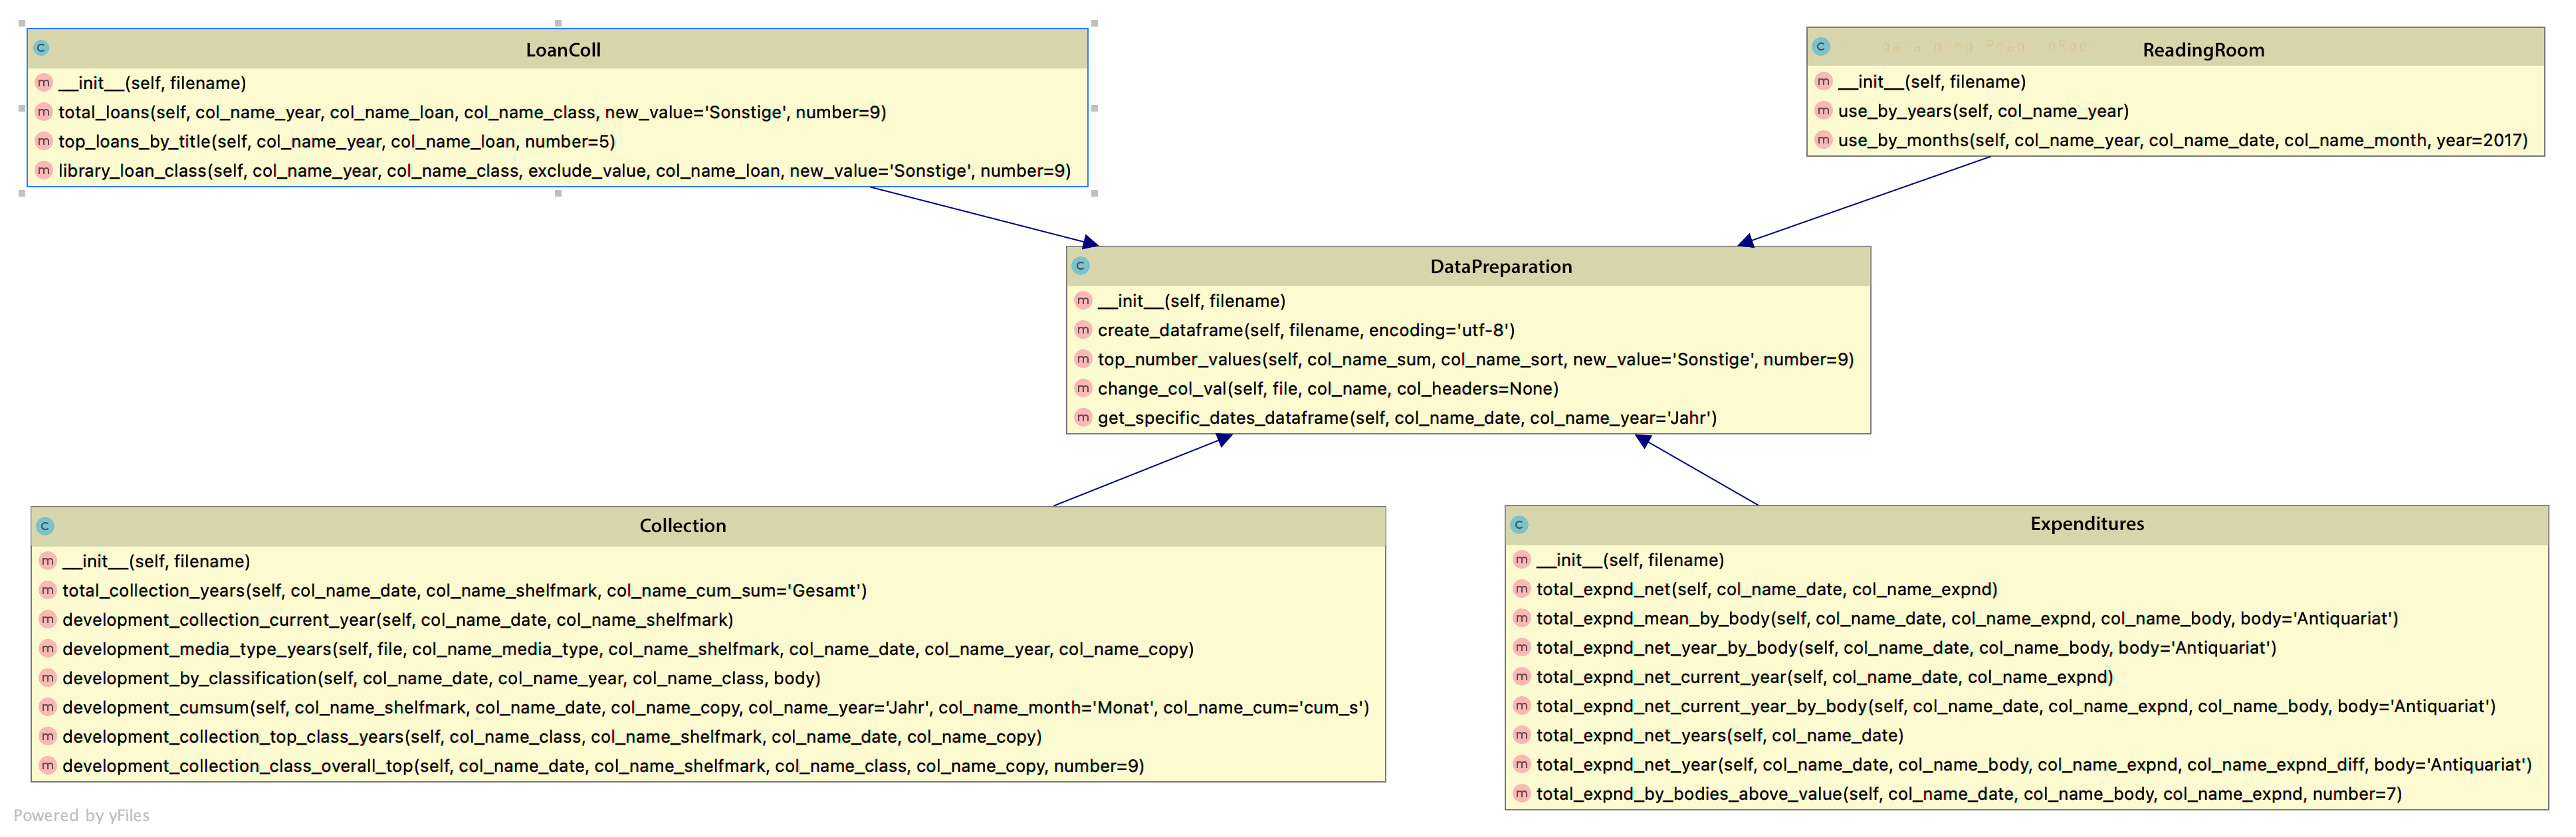
\includegraphics[width=21.5cm, height=12cm]{data_prep_class}
            \caption{Teilsystem 2 Datenbearbeitung - Klassen}
            \label{fig:classes data_prep}
    \end{sidewaysfigure}
    %\end{figure}

    Der Ablauf innerhalb des Teilsystems besteht aus zwei Schritten.\\
    (1) Das Laden der einzelnen CSV-Dateien aus dem Zielverzeichnis in die pandas Dataframes wird durch die Methode \texttt{create\_dataframe()} der Basisklasse geregelt.
    %Es wird noch einmal sichergestellt, dass die Daten in einem Zeichenformat wie utf-8 in das pandas Dataframe geladen werden.
    Beim Aufrufen des Konstruktors beziehungsweise der \texttt{init}-Methode der Klasse wird die Methode \texttt{create\_dataframe()} 
    automatisch mit aufgerufen. In den Kindklassen kann ebenfalls das Objekt mit dem pandas Dataframe instantiiert werden, da die Konstruktor-Properties der Basisklasse 
    an die Kindklassen mitvererbt werden. Die Objekte können nach Instantiierung durch die spezifischen Methoden der Kindklassen bearbeitet werden.
    
    (2) Das Ergebnis der Manipulation der pandas Dataframes ist auf die Darstellung der Daten im Dashboard ausgerichtet. Als Input für die einzelnen Methoden der
    Kindklassen werden verschiedene Parameter verlangt, mit deren Hilfe der Dataframe entweder manipuliert wird oder auf ihm Berechnungen ausgeführt werden können. 
    Um die Daten für das Teilsystem 3 vorzubereiten, können verschiedene Transformationsschritte auf den Daten innerhalb der Methoden ausgeführt werden. 
    Die Rückgabewerte der Methoden sind veränderte pandas Dataframes, pandas Series oder einzelne Skalare mathematischer Operationen.
    
    % Bei der folgenden Methode interessieren für die Darstellung im Dashboard nur die Umsatz/Budget-Daten für spezifische Datums-Daten. Hintergrund ist der, dass die 
    % monatlichen Umsatz- und Budgetdaten im Jahr akkumuliert werden. Wenn das Budget und der Umsatz nur Jahresweise dargestellt werden sollen, 
    % interessieren dementsprechend nur die Datensätze jeweils vom Dezember beziehungsweise vom aktuellen Monat im Jahr.
    

    % \begin{lstlisting}[language=Python, caption=Python example]
        
    %     def total_expnd_net_years(self, col_name_date):
    %         ...
    %         self._df = self.get_specific_dates_dataframe(col_name_date)
    %         return self._df

    % \end{lstlisting}
    

    % Die Methode \texttt{total\_expnd\_net\_years} der \texttt{Expenditures}-Klasse gibt nach einem Transformationsschritt einen pandas Dataframe zurück.
    % Der Transformationsschritt beinhaltet die Filterung des Dataframes nach spezifischen Werten in der Spalte des übergebenden Spaltennamens.
    % Zu diesem Zweck wird noch die Methode\\
    % \texttt{get\_specific\_dates\_dataframe} aufgerufen. 
    Anhand der folgenden Methode \texttt{total\_expnd\_net\_current\_year()} soll der zweite Schritt verdeutlicht werden.
    Die Methode der \texttt{Expenditures}-Klasse bestimmt im Allgemeinen die Summe von Werten einer Spalte, gefiltert
    nach einem Wert einer anderen Spalte ein und desselben pandas Dataframes. Mit dieser Methode soll so beispielsweise konkret der Gesamtumsatz des 
    laufenden Jahres bestimmt werden.

    \begin{lstlisting}[language=Python, caption=Teilsystem 2 Datenbearbeitung - total\_expnd\_net\_current\_year()]
    def total_expnd_net_current_year(self, col_name_date, col_name_expnd):
        ... 
        date_max = self._df[col_name_date].max()        
        self._df = self._df.set_index(col_name_date)
        self._df = self._df.loc[date_max]

        return self._df[col_name_expnd].sum()  
    \end{lstlisting}

    Als Input erwartet die Methode in der Methodensignatur zwei Spaltennamen als Parameter: den Namen der Datumspalte \texttt{col\_name\_date}, nach der gefiltert wird,
    und den Namen der Umsatz-Spalte \texttt{col\_name\_expnd}, auf der die Berechnung stattfindet. Der Transformationsprozess im Methodenkörper teilt sich in drei Schritte auf. Da die monatlichen Umsatzdaten pro Jahr als 
    akkumulierte Daten vorliegen, interessieren nur die Datensätze mit dem \enquote{größten} Datumswert. Deswegen
    wird nach diesen gefiltert und ein Dataframe von diesen erstellt. Dementsprechend wird mit der pandas-Funktion \texttt{max()} 
    zunächst der maximale Wert in der Datumsspalte bestimmt und der Variable \texttt{date\_max} zugewiesen. Danach wird in dem zweiten Schritt die Datumsspalte als Index gesetzt. 
    Im dritten Schritt wird der Dataframe mit den Reihen, die der Variable \texttt{date\_max} entsprechen, erstellt. Dies geschieht mit der pandas-Funktion \texttt{.loc}, die
    auf den Index der Reihen des Dataframes zugreift. Zum Schluss wird auf Basis der Umsatz-Spalte des Dataframes die Summe mit der pandas-Funktion \texttt{sum()} berechnet 
    und als Rückgabewert zurückgeliefert. Der Rückgabewert kann nun vom \textit{Teilsystem 3 Darstellung} weiterverarbeitet werden.\\

    \noindent
    \textit{Teilsystem 3 Darstellung}\\

    \begin{figure}[H]
        \centering
            \includegraphics[width=15cm, height=10cm]{Systemarchitektur_Ts3}
            \caption{Teilsystem 3 Darstellung - Systemarchitektur}
            \label{fig:Systemarchitektur Teilsystem 3}
    \end{figure}

    Für die Erstellung des Dashboards mit seinen Datenvisualisierungen und Interaktionen ist das \textit{Teilsystem 3 Darstellung} verantwortlich.
    In ihm werden die Ergebnisse des Teilsystems 2 zu Datenvisualisierungen verarbeitet und die Dashboard-Logik bereitgestellt.
    Die Bibliothek Plotly Express wird für die Datenvisualisierungen und die Bibliothek Dash zur Umsetzung des Dashboards genutzt. 
    Die Übergabe der Ergebnisse erfolgt durch den Aufruf der Objekte und der Methoden aus den Kindklassen des \texttt{data\_prep}-Moduls aus dem Teilsystem 2.
    %In ihm werden die Datenvisualisierungen mit den den Ergebnissen aus dem Teilsystem Datenbearbeitung
    %geschaffen. 
    
    Aufgrund der Vielzahl an Datenvisualisierungen im Dashboard wurde sich gegen eine Single-Page-Lösung entschieden. Deswegen besteht das Dashboard
    aus drei einzelnen Tabs, auf die die einzelnen Datenvisualisierungen aufgeteilt sind. Die Struktur der Dashboard-App entspricht einem Multi-App-Dashboard,
    für das es verschiedene Möglichkeiten gibt, es zu strukturieren.
    % Aufgrund der vielen Code-Blöcke tendieren Dashboards-Apps, die mit Dash geschrieben wurden zur Unübersichtlichkeit.
    Für das vorliegende Projekt wurde sich für die in 
    \autoref{fig:dash structure} gezeigte Struktur entschieden.

    \begin{figure}[H]
        \centering
            \includegraphics[width=6cm, height=3.5cm]{dash_struc}
            \caption{Teilsystem 3 Darstellung - Dashboard App - Struktur}
            \label{fig:dash structure}
    \end{figure}
    
    Dies ist eine Möglichkeit, wie sie auf der Webseite von Dash für diese Multi-App-Projekte vorgeschlagen wird \cite[vgl.][]{plotly_url_2021}.
    
    Für den Inhalt jedes einzelnen Tabs gibt es eine separate Datei.
    Die einzelnen Tabs wurden inhaltlich um bibliothekarische Basisfunktionen wie Sammeln oder Benutzen gruppiert. So werden in der \texttt{expenditures\_tab.py}
    Datenvisualisierungen erstellt, die Umsatz- und Budgetdaten visualisieren, während mit Hilfe der \texttt{loan\_read\_tab.py}
    Ausleih- und Lesesaalnutzungsdaten dargestellt werden. Mit der \texttt{newacq\_coll\_tab.py} wird ermöglicht, Daten aus dem Bereich der Bestandsentwicklung und der 
    Ausleihe zu präsentieren.

    Jede einzelne Tab-Datei besteht einerseits aus mehreren Funktionen für die Erstellung von Datenvisualisierungen der
    Ergebnisse aus Teilsystem 2.\footnote{ Zur besseren Lesbarkeit heißt die Gruppe dieser Funktionen im Folgenden \texttt{fig\_()}.}
    Innerhalb dieser Funktionen werden mit den Plotly-Funktionen Plotly Graph Object Figures geschaffen. 
    Andererseits bestehen die Dateien aus mehreren verschiedenen Funktionen für die Dash-Komponenten wie zum Beispiel Dropdown-Menüs, Cards oder Diagrammen.\footnote{ Ebenfalls zur besseren Lesbarkeit
    heißt die Gruppe dieser Funktionen im Folgenden \texttt{html\_()}.}
    Diese Funktionen binden die \texttt{fig\_()}-Funktionen so ein, dass die Plotly Graph Object Figures im Dashboard zur Anzeige gebracht werden können. 
    Weiterhin sind die \texttt{html\_()}-Funktionen zum Teil mit Dekorator-Callback-Funktionen verknüpft, die es ermöglichen, mit dem Dashboard zu interagieren. 
    Ferner enthalten die Dateien jeweils eine Layoutfunktion, die das gesamte Layout des Tabs bündelt.

    Neben den Funktionen für die Dash-Komponenten und der Datenvisualisierungen, werden in den tab-Dateien noch die benötigten Objekte aus dem Modul \texttt{data\_prep} 
    instantiiert und die Methoden der Kindklassen auf diese Objekte angewendet. In der Regel geschieht dies am Anfang 
    jeder Tab-Datei nach den Import-Anweisungen für die einzelnen Module außerhalb der Funktionen. Für die Callback-Funktionalität werden aber die Objekte und die Methoden des Moduls \texttt{data\_prep} innerhalb einiger \texttt{html\_()} aufgerufen.
    
    Auf den Aufbau und die Funktionsweise der Funktionen in den Tab-Dateien wird im Folgenden näher eingegangen.\footnote{ Auf die Erzeugung von anderen Dash-Elementen wie Cards wird dabei aufgrund der Übersichtlichkeit der Darstellung nicht Bezug genommen. Diesem liegt ein ähnlicher Prozess
    zu Grunde. Es werden aus den berechneten Ergebnissen der Objekte direkt Dash-Komponenten mit Hilfe der \texttt{dash\_bootstrap\_components} erstellt.}
    
    Die Objekte werden zunächst in Plotly Graph Objects umgewandelt. Diese wiederum werden in Dash-Objekte transformiert und diese werden 
    letztlich in einem Tab-Layout zusammengefasst.
    \autoref{fig:process tab} zeigt auf der nächsten Seite schematisch die Ablauflogik - aufgeteilt in vier Schritte - in den Tab-Dateien ohne die callback-Funktionen anhand der 
    \texttt{fig\_total\_expnd()}-Funktion aus der \texttt{expenditures\_tab.py}.
    
    
    \begin{figure}[H]
        \centering
            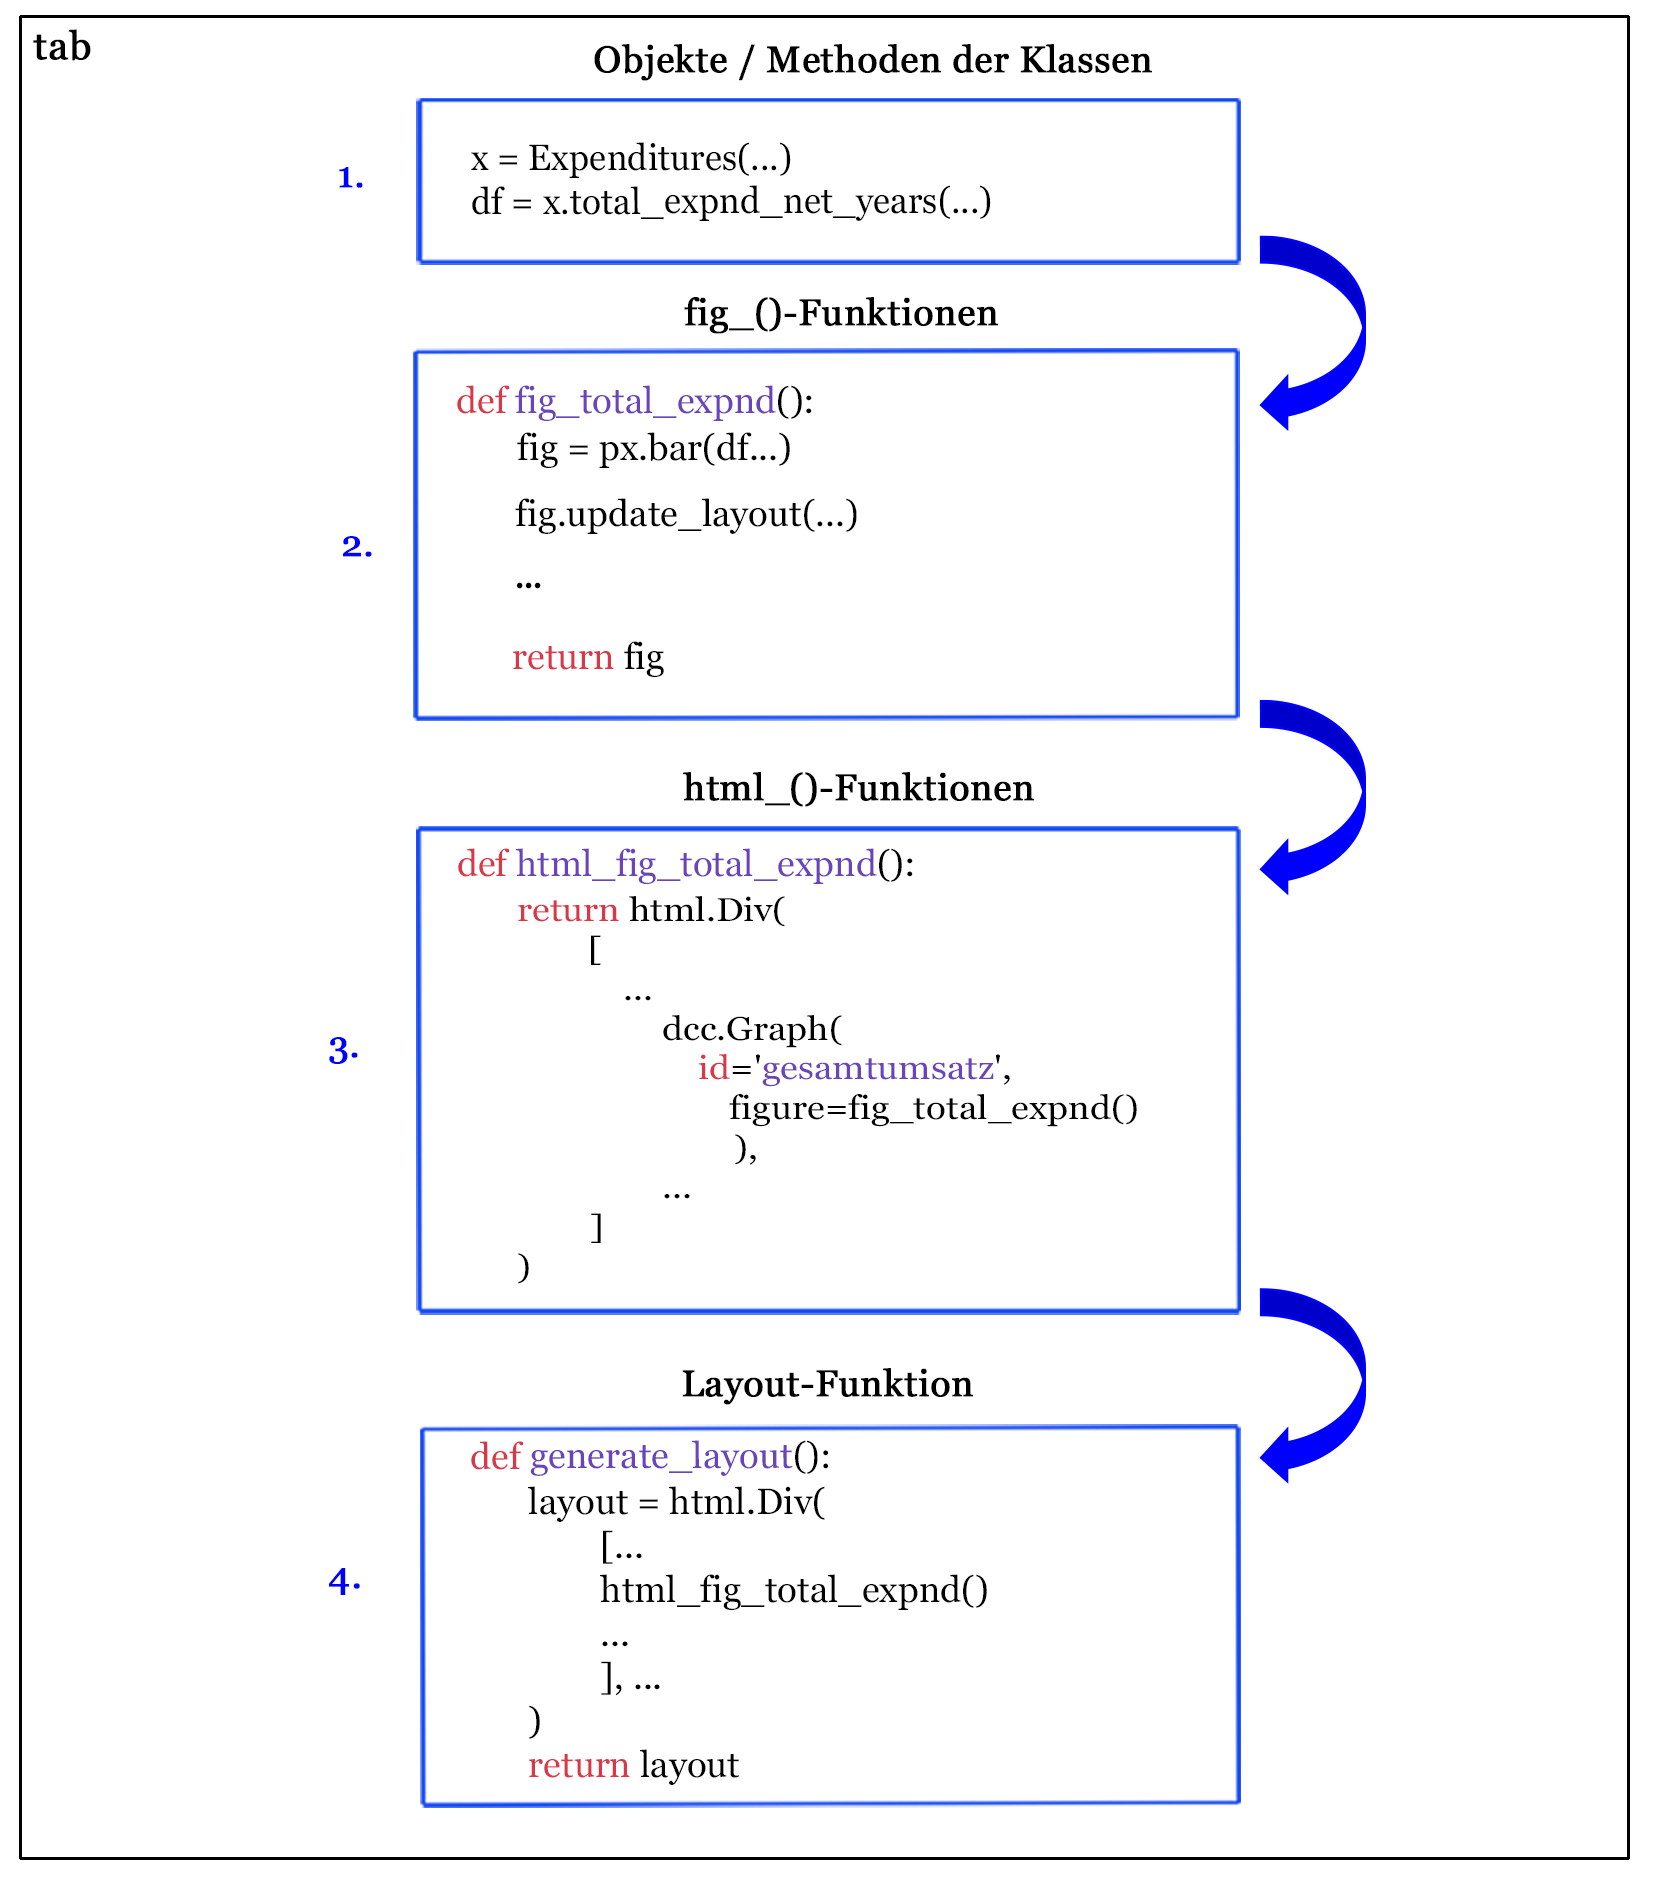
\includegraphics[width=12cm, height=16 cm]{ablauf_tab_ps}
            %\includegraphics[width=6cm, height=8cm]{ablauf_dash_ohne_cb}
            \caption{Teilsystem 3 Darstellung - Ablauf Tab}
            \label{fig:process tab}
    \end{figure}

    % Die grundsätzliche Logik der Funktionsaufrufe sieht in den Tab-Dateien ohne die Callback-Funktionen wie folgt aus:
    (1) Zunächst wird ein Objekt der Kindklasse \texttt{Expenditures()} aus dem \texttt{data\_prep}-Modul erzeugt 
    und auf ihm die Methode \texttt{total\_expnd\_net\_years()} ausgeführt und der Rückgabewert der Methode, der einem Dataframe entspricht, einer
    Variable zugewiesen.


    % \begin{figure}[H]
    %     \centering
    %         \includegraphics[width=10cm, height=8cm]{funktions_aufrufe_tab}
    %         \caption{Funktionsaufrufe Tab}
    %         \label{fig:function call tab}
    % \end{figure}

    (2) In der \texttt{fig\_}-Funktion, die das Plotly Graph Object Figure erzeugt, wird das durch die \texttt{total\_expnd\_net\_years()} erzeugte Dataframe
    als Parameter entgegengenommen. Zusätzlich müssen noch weitere Parameter übergeben werden, die für die jeweiligen Diagrammtypen wichtig sind.
    Andere Parameter, die das Layout festlegen, sind dagegen optional \cite[vgl.][]{plotly_plotlygraph_objectsbar_2021}.
    
    Im oben angegebenen Beispiel wird in der Funktion \texttt{fig\_total\_expnd()} aus \texttt{expenditures\_tab.py} ein horizontal gekipptes Figure-Objekt
    mit dem pandas Dataframe \texttt{df\_to-tal\_expnd} durch den Aufruf der Plotly-Funktion \texttt{bar()} erstellt. 
    Zusätzlich werden in dem Funktionsaufruf die x-Achse und y-Achse mit den Werten der Spalten \enquote{Umsatz (EUR)} und \enquote{Datum} festgelegt. 

    \begin{lstlisting}[language=Python, caption=Teilsystem 3 Darstellung - fig\_total\_expnd() Auszug 1]
    def fig_total_expnd():
        ...
        fig = px.bar(df_total_expnd,
            x='Umsatz (EUR)',
            y='Datum',
            orientation='h',
            ...
        )
        ...
    \end{lstlisting}
    
    Weitere Funktionen von Plotly Express bearbeiten die Plotly Graph Object Figures in den \texttt{fig\_()}-Funktionen. 
    So kann durch die \texttt{update\_layout}-Funktion unter anderem der Achsentitel, die Höhe und die Breite der Datenvisualisierung 
    festgelegt werden. Als Rückgabewert der Funktionen \texttt{fig\_()} werden die Plotly Graph Object Figures zurückgegeben.

    \begin{lstlisting}[language=Python, caption=Teilsystem 3 Darstellung - fig\_total\_expnd() Auszug 2]  
    def fig_total_expnd():
        ...
        fig.update_layout(title_x=0.5,
            xaxis_title='Umsatz (EUR)',
            yaxis_title='Jahr',
            height=500)
        fig.update_xaxes(nticks=20)         
        return fig
    \end{lstlisting}

    In dem Beispiel werden die Titel der x- und y-Achse sowie die
    Größe des Diagramm-Objektes festgelegt. Schließlich wird noch die x-Achse mit der Funktion \texttt{update\_xaxes()} skaliert.
    
    (3) Die \texttt{fig\_()}-Funktionen werden durch die Graph-Komponente der \texttt{dash\_core\_compo-nents} (dcc.Graph) innerhalb der 
    \texttt{html\_()}-Funktionen aufgerufen. Diese Komponente ist für die Umsetzung der interaktiven Datenvisualisierungen 
    zuständig. Ebenfalls kann von der Graph-Komponente eine \texttt{id} als Parameter entgegengenommen werden. 
    Diese ist unter anderem wichtig für die eindeutige Adressierung der Graph-Komponente durch die Callback-Funktionen.
    Zudem werden in den \texttt{html\_()}-Funktionen durch die \texttt{dash\_html\_components} die Eigenschaften und 
    das Aussehen der Div-Objekte definiert. 
    Dabei werden die Properties unter anderem in der externen css-Datei \texttt{layout.css} definiert, die in dem Unterverzeichnis \texttt{assets} 
    des Dashboard-Verzeichnisses liegt.

    \begin{lstlisting}[language=Python, caption=Teilsystem 3 Darstellung - html\_fig\_total\_expnd()] 
        def html_fig_total_expnd():
        ...
        return html.Div(
            [
                html.Div(
                    [
                        dcc.Graph(
                            id='gesamtumsatz',
                            figure=fig_total_expnd()
                        ),
                    ], className="six columns chart_div", style={'margin-top': '20px', 'margin-left': '10px'}
                ),
            ]
        )
        \end{lstlisting}
    
    (4) Die \texttt{html\_()}-Funktionen werden schließlich in einer Layoutfunktion eingebunden, die alle \texttt{html\_()}-Funktionen
    für das Gesamtlayout des Tab bündelt. Als Rückgabewert returniert sie ebenso wie die \texttt{html\_()}-Funktionen ein Div-Objekt der \texttt{dash\_html\_components}.\\



    Die Callback-Funktionen wurden für zwei Dropdown-Menüs in zwei Tab-Dateien implementiert.
    Die Werte der Dropdown-Menüs werden aus den uniquen Werten einer Dataframespalte erstellt.
    Der Callback ist als Dekorator für jeweils eine Funktion implementiert. 
    In der Implementierung wird ein Callback ausgelöst, wenn ein Wert über das Dropdown-Menü im Dashboard ausgewählt wird.
    Im Programmcode wird das für ein Diagramm der Lesesaalnutzung in der \texttt{loan\_read\_tab.py} folgendermaßen umgesetzt:

    \begin{lstlisting}[language=Python, caption=Teilsystem 3 Darstellung - update\_output\_div()]        
    
    @app.callback(
    Output(component_id='use_by_month', component_property='figure'),
    [Input(component_id='my-id2', component_property='value')])
    def update_output_div(input_value):
    ...
    return fig_use_by_month(input_value)
    \end{lstlisting}

    % Die Funktionsweise der Callback-Funktionen zeigt die \autoref{fig:process tab_dash_cb}.

    % \begin{figure}[H]
    %     \centering
    %         \includegraphics[width=8cm, height=10cm]{ablauf_dash_mit_cb}
    %         \caption{Ablauf Tab mit Callback}
    %         \label{fig:process tab_dash_cb}
    % \end{figure}
 
    Der Callback übergibt den Wert (input\_value) des Dropdown-Menüs an die Funktion \texttt{update\_output\_div()}. 
    Die Funktion gibt das Ergebnis einer \texttt{fig\_()}-Funktion mit diesem Wert als Argument zurück.\footnote{ Diese Funktionen übergeben den Methoden der Kindklassen aus dem Modul \texttt{data\_prep} das Argument. 
    Diese erzeugen einen Dataframe basierend auf den übergebenden Argument und geben mit Hilfe der Plotly-Funktionen ein Plotly Graph Object Figure der gefilterten Daten zurück.}
    Der Callback \texttt{@app.callback} übergibt das zurückgegebene Ergebnis an die im Output angegebene Komponente.
    
    Input() und Output() nehmen die id einer Komponente und die Eigenschaft einer Komponente als Argumente entgegen.
    Die Inputkomponente ist in dem angeführten Beispiel die Dropdown-Komponente, während die Outputkomponente die dcc.Graph-Komponente der
    \texttt{html\_use\_by\_month()} darstellt. Beide werden über die eindeutige \texttt{component\_id} adressiert.
    Multiple Inputs and Outputs sind ebenfalls möglich. So sind in der \texttt{expenditures\_tab.py}
    jeweils zwei Diagramme und Zahlenwerte für den Umsatz von den Werten eines Dropdown-Liste abhängig.
    % Dabei handelt es sich um Methoden, die die Daten nach einem Wert filtern und die vom Wert der Dropdown-Liste abhängig sind. Deswegen wird bei diesen
    % Plotly-Funktionen in der Tab-Datei der Wert der Dropdown-Liste als Argument mit in die Funktion gegeben.
    In der \autoref{fig:process tab_dash_cb} ist die Ablauflogik in den Tab-Dateien mit der Callback-Funktion skizziert.

    \begin{figure}[H]
        \centering
            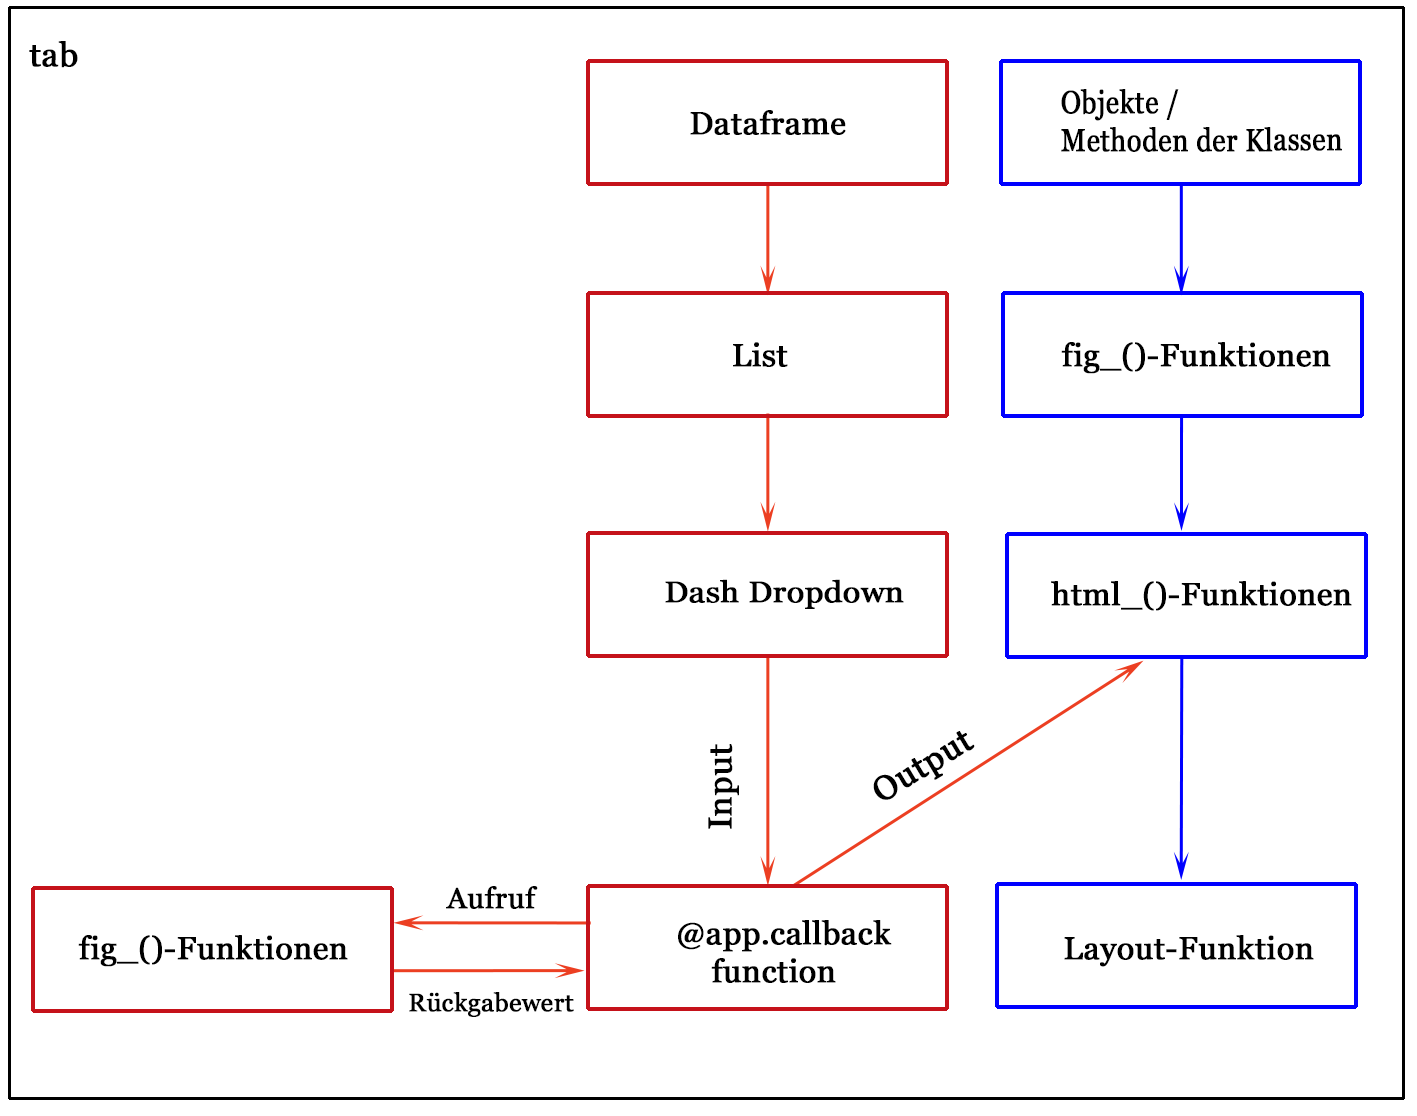
\includegraphics[width=12cm, height=10cm]{ablauf_tab_cb_ps}
            \caption{Teilsystem 3 Darstellung - Ablauf Tab mit Callback}
            \label{fig:process tab_dash_cb}
    \end{figure}


    Zusammengesetzt wird das Layout des Dashboards durch den Aufruf der Layout-Funktion der einzelnen Tab-Dateien in der \texttt{index.py}.
    Die \texttt{index.py} definiert zudem das Layout des gesamten Dashboards. Hier werden auch die Anzahl und die Eigenschaften der Tabs festgelegt. 
    Die Dekorator-Callback-Funktion \texttt{@app.callback()} der \texttt{index.py} steuert die Auswahl der Tabs und ruft die jeweiligen Tabs beziehungsweise deren 
    Layouts auf. \autoref{fig:process tab_dash_cb_ind} zeigt die Funktionsweise einer Tab-Datei mit der \texttt{index.py}.

    \begin{figure}[H]
        \centering
            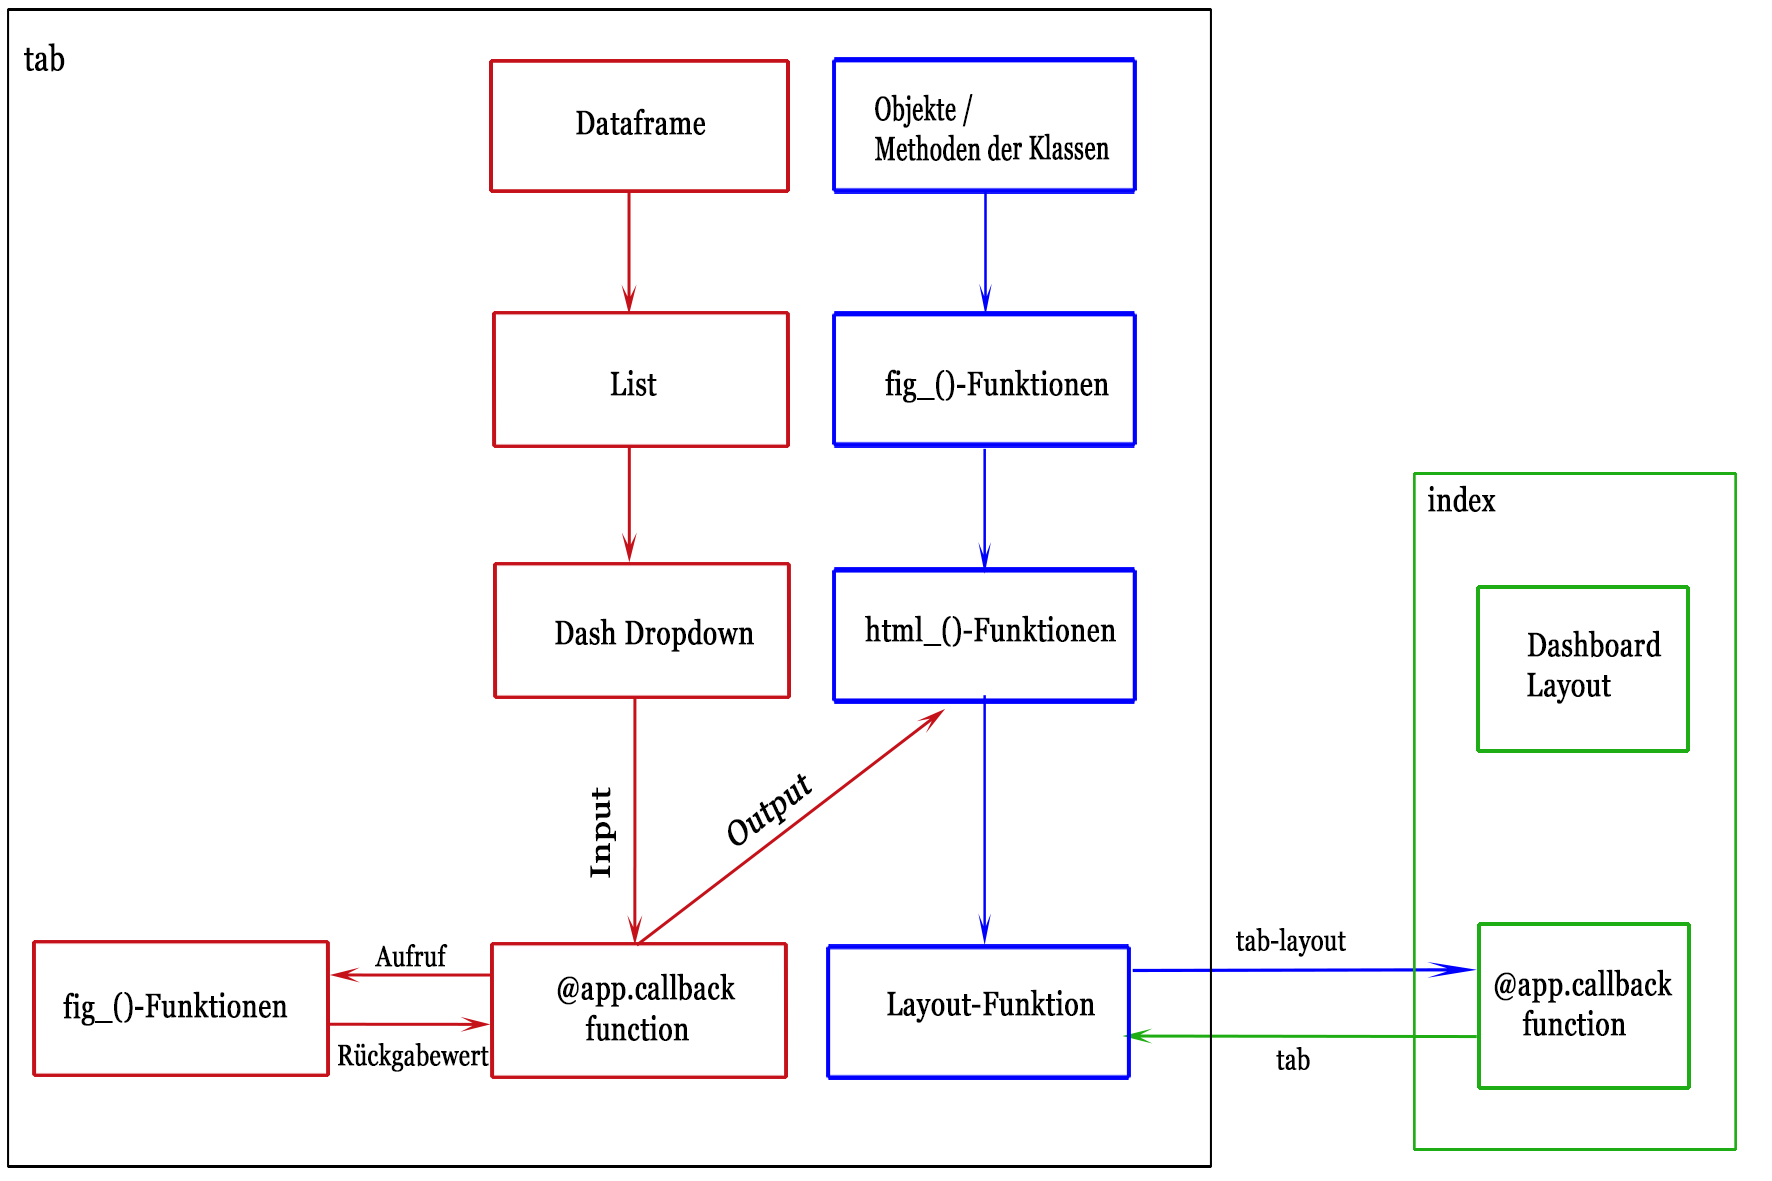
\includegraphics[width=15cm, height=10cm]{ablauf_tab_cb_ind_ps}
            \caption{Teilsystem 3 Darstellung - Ablauf Tab mit index.py}
            \label{fig:process tab_dash_cb_ind}
    \end{figure}

    Der Einstiegspunkt zur Ausführung des Dashboards ist die Datei \texttt{index.py}. Mit dieser Datei wird das Dashboard mittels \texttt{Flask-Webserver}
    gestartet. Zur Vermeidung zirkulärer Importe ist die Dash-Instanz in der separaten \texttt{app.py} definiert \cite[vgl.][]{plotly_url_2021}.


    %\textit{Standardbericht}\\

\section{Demonstration der Funktionalität}

    Im Folgenden wird die Funktionsweise des Systems dargelegt. 
    Dabei wird zunächst auf die technischen Voraussetzungen eingegangen.
    Nach einer Erläuterung des Teilsystems 1 Import wird schließlich der
    praktische Import der Daten skizziert. Da das Teilsystem 2 keine Schnittstelle
    nach außen bietet, wird auf dieses nicht eingegangen. Das Teilsystem 3 ist insofern interessant, da von diesem das Dashboard
    gestartet wird. Das Dashboard ist die graphische Umsetzung der Teilsysteme 2 und 3.
    Es wird kurz auf das Layout des Dashboards eingegangen, bevor die Funktionsweise und die Datenvisualisierungen besprochen werden.


    \subsection{Technische Voraussetzungen}
    Der Programmcode zum Projekt ist auf GitHub zu finden.\footnote{ \url{https://github.com/pbretern/library-dashboard-system} v1.0} Dort gibt es weitere Informationen zur Installation.
    Das System wurde auf den Betriebssystemen macOS Big Sur und Linux in der Ubuntu-Distribution 20.10. getestet.
    Das Dashboard kann mit den aktuellen Versionen\footnote{ Stand: 06.03.2021} der Web-Browser Google Chrome, Firefox und Safari dargestellt werden. 
    Als Hardware-Anforderungen wird ein Intel Dual Core i5 (Haswell) mit 128 GB Festplatte und 8 GB Arbeitsspeicher angegeben. 
    Mit dem Programmcode werden keine Originaldaten aus der Bibliothek mitgeliefert.\footnote{ Wenige Testdaten für das Dashboard werden mit der Veröffentlichung des Repositoriums
    bereitgestellt. Es stehen mit der v1.0 pseudonymisierte und randomisierte Umsatz- und Budgetdaten zur Verfügung.}
    
    \subsection{Daten-Import}
    Der Import der Daten findet über Skripte statt. Diese liegen im Projektverzeichnis \texttt{src/instances}.
    Für Budget, Umsatz, Neuerwerbungen und Ausleihdaten liegen einzelne Python-Skripte bereit, die manuell über die Kommandozeile
    aufgerufen werden können. Zudem gibt es noch ein shell-Skript, das die vier Skripte zusammen auslöst. Dieses
    muss ebenfalls manuell aufgerufen werden.
    Beim Import wird eine Meldung über die Anzahl der zu importierenden Daten auf der Kommandozeile angezeigt. 
    Nach erfolgreichem Abschluss des Imports wird zudem eine einfache Erfolgsmeldung auf der Kommandozeile ausgegeben.
    %\footnote{  Es gibt Warnungen, die angezeigt werden. Diese Warnmeldungen haben keinen Einfluss auf den Import. Im Bearbeitungszeitraum der Arbeit konnte diesen Warnmeldungen leider nicht nachgegangen werden.}

    Die Pfade zu den lokalen Verzeichnissen für Import und Speicherung der Daten sind als Konstanten zentral in der \texttt{configuration.py}
    im Projektverzeichnis hinterlegt. Dort sind auch noch andere Pfadkonstanten definiert, die auf Dateien für die Datenanreicherung verweisen, welche das Teilsystem 1
    und das Teilsystem 2 unterstützen. Wichtig ist, dass die zu importierenden Daten über Dateinamen einer gewissen Semantik und 
    über ein gewisses Format verfügen müssen, sonst werden sie nicht importiert (Siehe auch \autoref{chap:five_one_three}, Teilsystem 1).

    \subsection{Dashboard}
    Gestartet wird die Dashboard-Applikation auf der Kommandozeile, indem die Datei \texttt{index.py} im Projektverzeichnis \texttt{dashboard}
    aufgerufen wird. Diese startet den Flask-Webserver mit der Dashboard-App. Der Webserver ist in der \texttt{index.py} so eingestellt, 
    dass er alle Netzwerkschnittstellen abhört.


    \begin{figure}[H]
        \centering
            \includegraphics[width=12cm, height=2cm]{flask_webserver}
            \caption{Teilsystem 3 Darstellung - Flask Webserver}
            \label{fig:flask}
    \end{figure}

    % Wie im \autoref{chap:five_one_three} Teilsystem 3 beschrieben besteht das Dashboard aus drei Tabs.
    % Die Navigation zu den drei Tabs ist im oberen Bereich des Dashboards nebeneinander angeordnet. 
    
    % \begin{figure}[H]
    %     \centering
    %         \includegraphics[width=14cm, height=2cm]{tabs}
    %         \caption{Tabs-Navigation}
    %         \label{fig:flask}
    % \end{figure}
    Das Dashboard kann mit der angegebenen Adresse vom Web-Browser geöffnet werden.
    \autoref{fig:Struktur Layout} zeigt auf der folgenden Seite schematisch die Layout-Struktur des Dashboards. 


    \begin{figure}[H]
        \centering
            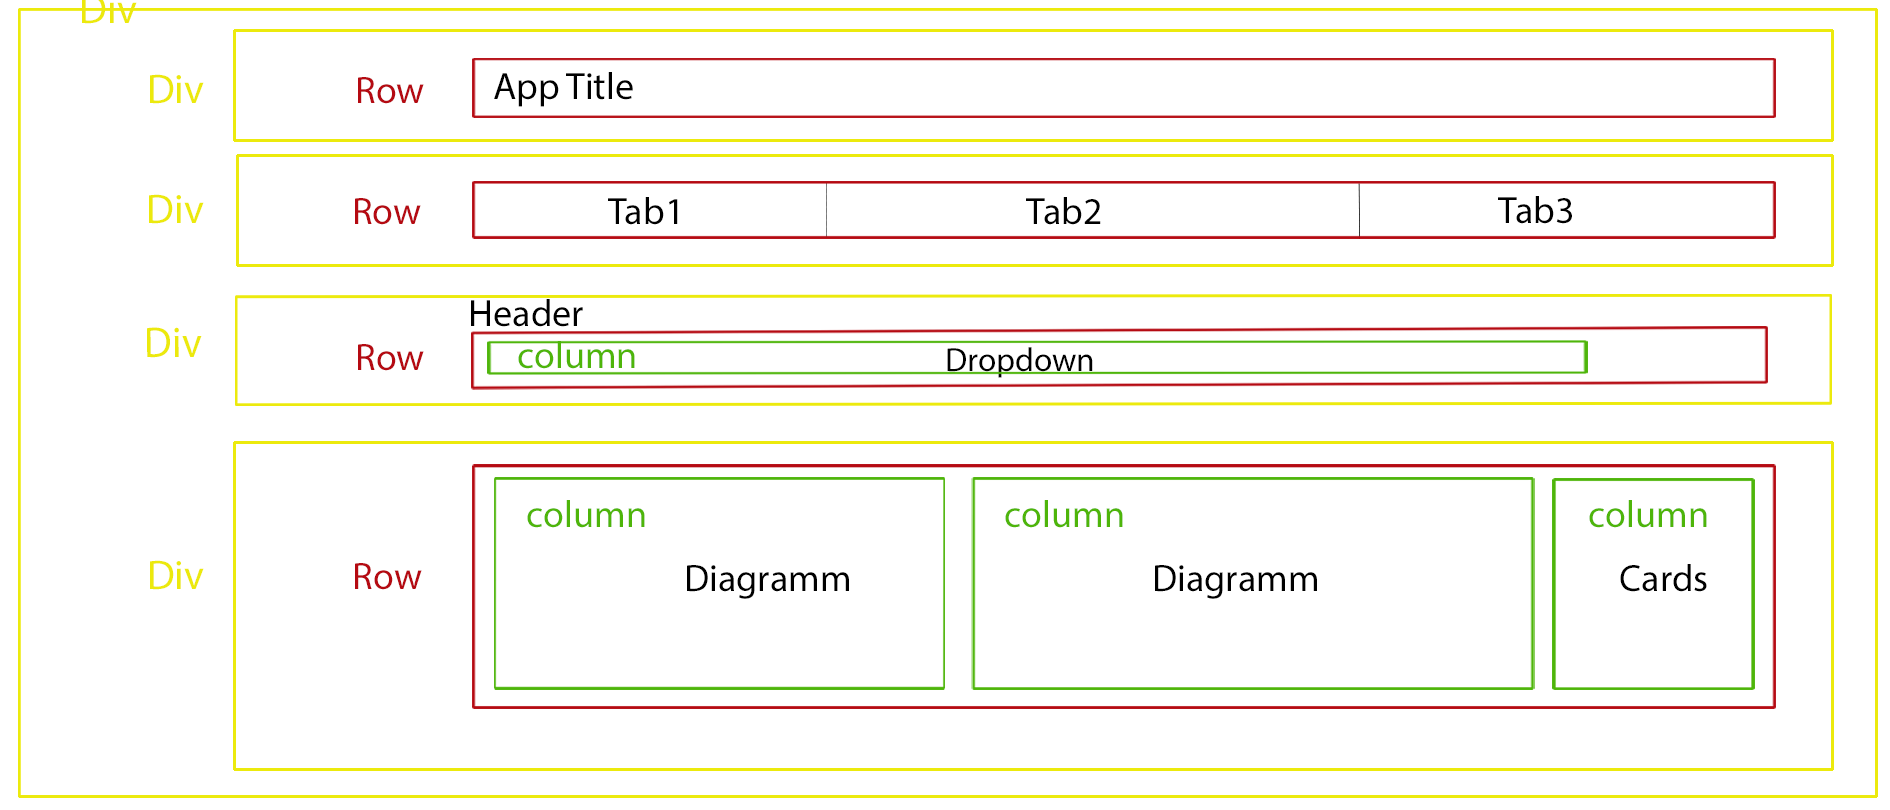
\includegraphics[width=14cm, height=6cm]{layout_abstr}
            \caption{Teilsystem 3 Darstellung - Dashboard Layout - Struktur}
            \label{fig:Struktur Layout}
    \end{figure}


    Die Layout-Struktur besteht aus Divs, Rows, Header und Columns, den Steuerelementen wie Dropdown-Menüs sowie den Darstellungselementen wie Diagramme, Tabellen
    oder Cards. Die einzelnen Rows werden durch Div-Container bemantelt. Diese sind auf dem html-Body angesiedelt.
    Während die ersten beiden Rows zentral in der \texttt{index.py} festgelegt werden, werden die anderen Rows in den einzelnen Tab-Dateien definiert. 
    Diese Rows beherbergen bis zu drei Columns-Elemente, in denen die Steuer- und Datenvisualisierungselemente enthalten sind.
    Die Columns-Elemente sind in Abhängigkeit der darzustellenden Daten unterschiedlich groß. 
    Die Größe wird festgelegt in den einzelnen \texttt{fig\_()}-Funktionen des Teilsystems 3.
    Die Header gelten als inhaltlicher Trenner zwischen den einzelnen Datenvisualisierungen und dienen der schnelleren Orientierung. 
    Die Header sind zudem mit der jeweils nachfolgenden Row verknüpft. Das Dashboard besteht aus drei Tabs: \textit{Umsatz und Budget}, 
    \textit{Lesesaal und Ausleihe}, \textit{Neuerwerbungen und Bestand}. Der Wechsel zwischen den Tabs geschieht durch das einmalige
    Klicken mit der Maus auf dem Tab-Titel. Nachdem die Adresse im Browser geöffnet wurde, wird der Tab \textit{Umsatz und Budget} aufgerufen. Dieser ist
    als default-value im Dashboard-Layout der \texttt{index.py} eingestellt. Im Folgenden werden die Tabs per screenshot abgebildet sowie 
    die in ihnen enthaltenen Informationen tabellarisch dargestellt. Die tabellarische Darstellung richtet sich dabei an den Rows der Layout-Struktur aus. 

    %\clearpage
    % \noindent
    % \textit{Tab1 - Umsatz und Budget}
    % %Den Tab \textit{Umsatz und Budget} zeigt \autoref{fig:tab1}
    % \footnote{  Für die Darstellung der Umsatz- und
    % Budgetdaten werden sowohl die Kostenstellen als auch die Lieferanten maskiert dargestellt. Es wurde außerdem mit Testdaten
    % gearbeitet, die bis März 2021 gehen.}

    \KOMAoptions{paper=A3,paper=portrait}
    \recalctypearea
    
    \textit{Tab1 - Umsatz und Budget}\footnote{  Für die Darstellung der Umsatz- und
    Budgetdaten werden sowohl die Kostenstellen als auch die Lieferanten pseudonymisiert dargestellt. Die Zahlen
    wurden randomisiert.}
    %\begin{sidewaysfigure}
    \begin{figure}[H]
        \centering
            \includegraphics[width=22cm, height=26 cm]{tab1_2}
            \caption{Screenshot Tab1 - Umsatz und Budget}
            \label{fig:tab1}
    \end{figure}
    %\end{sidewaysfigure}

    % Genug A3 fürs erste. Jetzt ein Seitenumbruch und dann wieder A4-Format:
    \clearpage
    \KOMAoptions{paper=A4,paper=portrait}
    \recalctypearea  
    %Folgende Diagramme und Steuerelemente werden im Tab \textit{Umsatz und Budget}.
    \begingroup
    \setlength{\tabcolsep}{12pt} % Default value: 6pt
    \renewcommand{\arraystretch}{1.5}
    \begin{table}[h]
        \LARGE
        \centering
        \begin{adjustbox}{max width=\textwidth}
        \begin{tabular}{p{0.1\textwidth}p{0.5\textwidth}p{0.4\textwidth}p{0.25\textwidth}p{0.4\textwidth}p{0.5\textwidth}}
           \toprule
           Row        &Titel der Darstellung&Beschreibung &Datenset &Darstellung &Interaktivität auf dem Dashboard\\
           \midrule
            1           &Gesamtumsatz Lieferanten nach Jahren &Die Einzelwerte der Lieferanten pro Jahr werden dargestellt.   &Umsatzdaten    &gestapeltes Balkendiagramm (horizontal)    &Plotly-Interaktivität (Aus- und Einblenden von Balken, Hover-Informationen).\\
                        &Top 10 Lieferanten mit Sonstige &Die 9 Lieferanten, bei denen der Umsatz am stärksten ist, werden dargestellt. Die restlichen werden in Sonstiges gruppiert.   &Umsatzdaten    &Balkendiagramm    &Plotly-Interaktivität (Aus- und Einblenden von Balken, Hover-Informationen).\\
                        &Gesamtumsatz&-&Umsatzdaten    &numerischer Wert   &-\\
                        &Gesamtumsatz laufendes Jahr&-&Umsatzdaten    &numerischer Wert   &-\\
            
                        \midrule
            2           &Auswahl  Lieferant &Dropdown-Menü mit eindeutigen Werten der Dataframe-Spalte \enquote{Lieferanten Abk.}&Umsatzdaten&Dropdown-Menü &Auswahl von Werten aus einer Liste. Dadurch werden vier Darstellungen im Tab beeinflusst.\\
            \midrule
            3           &Gesamtumsatz Lieferant nach Jahren&Der Gesamtumsatz eines Lieferanten nach Jahren wird dargestellt.   &Umsatzdaten    &Balkendiagramm    &Auswahl des Lieferanten über das Dropdown-Menü.\\
                        &Lieferant Umsatz pro Monat laufendes Jahr&Der Gesamtumsatz eines Lieferanten nach Monaten für das laufende Jahr wird dargestellt.   &Umsatzdaten    &Balkendiagramm    &Auswahl des Lieferanten über das Dropdown-Menü.\\
                        &Umsatz laufendes Jahr (für einen Lieferanten)&- &Umsatzdaten    &numerischer Wert    &Wert verändert sich durch Auswahl des Lieferanten über das Dropdown-Menü.\\
                        &Jahresdurchschnitt (für einen Lieferant)&- &Umsatzdaten    &numerischer Wert    &Wert verändert sich durch Auswahl des Lieferanten über das Dropdown-Menü.\\
            \midrule
            4           &Gesamtbudget Kostenstellen nach Jahren&Die Einzelwerte der Kostenstellen pro Jahr werden dargestellt.&Budgetdaten    &gestapeltes Balkendiagramm (horizontal)    &Plotly-Interaktivität (Aus- und Einblenden von Balken, Hover-Informationen).\\
                        &Top 5 Kostenstellen mit Sonstige&Die 4 Kostenstellen, bei den die Budgetkosten am größten sind, werden dargestellt. Die restlichen werden in der Sonstiges gruppiert. &Budgetdaten    &Kreisdiagramm    &Plotly-Interaktivität (Aus- und Einblenden von Anteilen, Hover-Informationen).\\

        \bottomrule
        \end{tabular}
        \end{adjustbox}
        \caption
        \end{table}
    \endgroup
    


\clearpage
\KOMAoptions{paper=A3,paper=portrait}
\recalctypearea
\textit{Tab2 - Lesesaal und Ausleihe}\footnote{ Die Skalen und Legenden der Diagramme sowie die Tabelle wurden unkenntlich gemacht.
Das Diagramm \enquote{Gesamtverteilung Ausleihe Buchservice / Bibliothek} wurde verfremdet.}
%Den Tab \textit{Lesesaal und Ausleihe} zeigt \autoref{fig:tab2}.
    \begin{figure}[H]
        \centering
            \includegraphics[width=22cm, height=26cm]{tab2}
            \caption{Screenshot Tab2 - Lesesaal und Ausleihe}
            \label{fig:tab2}
    \end{figure}

\clearpage
\KOMAoptions{paper=A4,paper=portrait}
\recalctypearea  

%\clearpage
%Folgende Diagramme, Tabellen und Steuerelemente werden im Tab \textit{Lesesaal und Ausleihe} dargestellt.
    \begingroup
    \setlength{\tabcolsep}{12pt} % Default value: 6pt
    \renewcommand{\arraystretch}{1.5} 
    \begin{table}[h]
        \LARGE
        \centering
        \begin{adjustbox}{max width=\textwidth}
        \begin{tabular}{p{0.1\textwidth}p{0.5\textwidth}p{0.4\textwidth}p{0.3\textwidth}p{0.4\textwidth}p{0.4\textwidth}}
           \toprule
           Row        &Titel der Darstellung&Beschreibung &Datenset &Darstellung &Interaktivität auf dem Dashboard\\
           \midrule
            1           &Auswahl  Jahr &Dropdown-Menü mit eindeutigen Werten der Dataframe-Spalte \enquote{Jahr}.&Ausleihdaten&Dropdown-Menü &Auswahl von Werten aus einer Liste. Dadurch wird eine Darstellung beeinflusst.\\
           \midrule
            2           &Monatliche Anzahl der Nutzer:innen nach Service-Zeiten&Es wird der monatliche Verlauf pro Jahr nach den vier Service-Zeiten-Gruppen dargestellt.&Lesesaaldaten&Liniendiagramm&Auswahl des Zeitraums (Jahr) über Dropdown-Menü. Plotly-Interaktivität (Aus- und Einblenden von Linien, Hover-Informationen).\\
                        &Jährliche Lesesaalnutzung nach Service-Zeiten&Es wird die jährliche Nutzung des Lesesaal in den Service-Zeiten-Gruppen dargestellt.&Lesesaaldaten&Balkendiagramm    &Plotly-Interaktivität (Aus- und Einblenden von Balken, Hover-Informationen).\\          
            \midrule
            3           &Ausleihe Top RVK-Fachsystematiken mit Buchservice und Sonstige&Die 8 \textit{\acrshort{RVK}}-Fachsys-tematiken, bei denen die Ausleihanzahl am größten ist werden dargestellt. Die übrigen Fachsystematiken im Bestand werden in Sonstiges gruppiert. Buchservice wird auch dargestellt.&Ausleihdaten&gestapeltes Balkendiagramm (horizontal)&Plotly-Interaktivität (Aus- und Einblenden von Balken, Hover-Informationen).\\
                        &Gesamtverteilung Ausleihe Buchservice / Bibliothek&Es wird die prozentale Verteilung zweier Werte dargestellt.&Ausleihdaten    &Kreisdiagramm   &Plotly-Interaktivität (Aus- und Einblenden von Anteilen, Hover-Informationen).\\
            \midrule
            4           &Tabellarische Darstellung der 5 besonders nachgefragten Titel nach Jahren&-&Ausleihdaten    &Tabelle mit den Spalten Jahr, Signatur, Titel und Anzahl der Ausleihen.&-\\

        \bottomrule
        \end{tabular}
        \end{adjustbox}
        \caption
        \end{table}
    \endgroup

\clearpage
    
    
    %Den Tab \textit{Neuerwerbungen und Bestand} zeigt \autoref{fig:tab3}.

    \KOMAoptions{paper=A3,paper=portrait}
    \recalctypearea
    \textit{Tab3 - Neuerwerbungen und Bestand}\footnote{ Die Skalen und Legenden der Diagramme wurden unscharf gemacht.}
    \begin{figure}[H]
        \centering
            \includegraphics[width=22cm, height=26cm]{tab3}
            \caption{Screenshot Tab3 - Neuerwerbungen und Bestand}
            \label{fig:tab3}
    \end{figure}

    %\clearpage
    \KOMAoptions{paper=A4,paper=portrait}
    \recalctypearea 
    %Folgende Diagramme werden im Tab \textit{Neuerwerbungen und Bestand} dargestellt.
    \begingroup
    \setlength{\tabcolsep}{12pt} % Default value: 6pt
    \renewcommand{\arraystretch}{1.0} 
    \begin{table}[H]
        \LARGE
        \centering
        \begin{adjustbox}{max width=\textwidth}
        \begin{tabular}{p{0.1\textwidth}p{0.5\textwidth}p{0.4\textwidth}p{0.3\textwidth}p{0.4\textwidth}p{0.4\textwidth}}
           \toprule
           Row        &Titel der Darstellung&Beschreibung &Datenset &Darstellung &Interaktivität auf dem Dashboard\\
           \midrule
            1           &Monatliche Neuerwerbungen laufendes Jahr&Es werden die monatlichen Neuerwerbungen des laufenden Jahres dargestellt.&Bestandsdaten&Balkendiagramm&-\\
                        &Jährliche Bestandsentwicklung nach Monaten&Darstellung des akkumulierten Bestandswachstums für die einzelnen Jahre&Bestandsdaten&Liniendiagramm    &Plotly-Interaktivität (Aus- und Einblenden von Linien, Hover-Informationen)\\          
            \midrule
            2           &Bestandswachstum pro Jahr und Gesamt&Darstellung des absoluten und des relativen Wachstums nach Jahren.&Bestandsdaten&überlagertes Balkendiagramm&Plotly-Interaktivität (Aus- und Einblenden von Balken, Hover-Informationen)\\
                        &Top 10 RVK-Fachsyste-matiken pro Jahr&Die jährlichen Top 10 \textit{\acrshort{RVK}}-Fachsys-tematiken im Bestand werden dargestellt.&Bestandsdaten    &gestapeltes Balkendiagramm&Plotly-Interaktivität (Aus- und Einblenden von Balken, Hover-Informationen)\\
            \midrule
            3           &Top RVK-Fachsystema-tiken Ausleihe mit Sonstige&Es werden 9 \textit{\acrshort{RVK}}-Fachsyste-matiken der Ausleihe vom kleinsten Wert zum größten des Bestandes (ohne Buchservice) dargestellt. Die übrigen Systematiken werden in Sonstige dargestellt.&Ausleihdaten&Balkendiagramm&Plotly-Interaktivität (Aus- und Einblenden von Balken, Hover-Informationen)\\
                        &Top RVK-Fachsystema-tiken Bestand mit Sonstige&Es werden  9 \textit{\acrshort{RVK}}-Fachsyste-matiken im Bestand vom größten Wert zum kleinsten dargestellt. Die übrigen Systematiken werden in Sonstige dargestellt.&Bestandsdaten&Balkendiagramm&Plotly-Interaktivität (Aus- und Einblenden von Balken, Hover-Informationen)\\

        \bottomrule
        \end{tabular}
        \end{adjustbox}
        \caption
        \end{table}
    \endgroup

\section{Bewertung}

\subsection{Allgemeines}
\label{chap:five_three_one}
Das Ziel des vorliegenden Projektes war es, ein Proof-of-Concept eines Systems zu entwickeln, 
das wesentliche bibliothekarische Daten sammelt, statistisch mit geeigneten Methoden und
Datenvisualisierungen analysiert. Als Ergebnis steht ein datengetriebenes 
Unterstützungssystem, das durch drei Teilsysteme den Import und eine erste Bereinigung der Daten,
die Aufbereitung der Daten, die Umwandlung der Daten in Datenvisualisierungen und deren Darstellung garantiert. 
Das System verarbeitet bibliothekarische Daten aus den Bereichen Umsatz und Budget, Lesesaal und Ausleihe 
sowie der Bestandsentwicklung. Es wurde vor dem Hintergrund der regelmäßigen Datenbereitstellung entwickelt.

Das System ist ausgelegt auf diese bibliothekarischen Daten, die aus heterogenen Datenquellen stammen.
Diese Daten bringen spezifische Anforderungen wie Datenbeschaffenheit oder Dateiformatspezifikationen mit, 
die den Prozess der Datenintegration in das System bestimmen. Es konnte mit dem System gezeigt werden, 
dass diese Anforderungen für die vorliegenden Daten vom System erfüllt wurden, indem entsprechende Prozesse innerhalb
der drei Teilsysteme für diese Daten entwickelt wurden.

So erwartet das System beim Import die Daten in einer gewissen Struktur (Datenformat). 
Überdies muss das Dateiformat dem System bekannt sein und der Dateiname speziellen semantischen 
Kriterien entsprechen. Wenn diese Anforderungen erfüllt sind, können die Daten problemlos in das System integriert werden.
Weiterhin können bestimmte Modifikationen eingestellt werden wie die Entfernung
bestimmter Zeichen im Teilsystem 1. Diese Modifikationen sind aber sehr einfach und wurden aus der Voranalyse
der Daten entwickelt. Die Modifikationen können zwar auf andere Daten angewendet werden, gelten aber in erster Linie nur für die vorliegenden Daten. 
Darüber hinaus bietet das System im Teilsystem 1 keine weiteren einstellbaren Möglichkeiten an. Ferner ist das System auf einfache 
Tabellenstrukturen, wie sie in TSV- oder Excel-Dateien abgespeichert werden können, ausgerichtet.
Grundsätzlich erfolgt der Import der Daten (einfache Tabellenstrukturen) aus heterogenen Datenquellen 
in einfache Tabellenstrukturen in einem einheitlichen CSV-Dateiformat. Der einfache Import von Daten aus einem Dateiformat 
in das CSV-Format ist aber problemlos möglich, wenn Daten vorliegen, die keine weiteren speziellen
Anforderungen besitzen.

Das Teilsystem 2 und das Teilsystem 3 erwarten CSV-Dateien, die sie weiterverarbeiten können. 
Deshalb kann das datengetriebene Unterstützungssystem auch unabhängig vom Teilsystem 1 funktionieren. 
Das Teilsystem 1 stellt vielmehr eine Möglichkeit dar, wie der Import der Daten ablaufen kann. 
Das Teilsystem 1 wurde für das System entwickelt, da insbesondere mit den vorliegenden Daten umgegangen werden musste und ebenfalls hier 
der Großteil der Datenanreicherung abläuft.


\subsection{Datenlage im vorliegendem System}
In dem vorliegenden Projekt wurden hauptsächlich die heterogenen Bibliotheksdaten aus dem \textit{\acrshort{hebis}}-Verbund sowie aus dem \textit{\acrlong{LBS}} Frankfurt verarbeitet.
Da potentiell alle Bibliotheken, die durch das \textit{\acrshort{LBS}}-Team Frankfurt betreut werden, die gleichen Daten zur Verfügung gestellt bekommen,
kann das vorliegende  System von diesen Bibliotheken implementiert werden. Eine Aussage darüber, ob es in anderen Bibliotheken oder Verbünden implementiert werden kann, die ebenfalls
Instanzen des \textit{\acrlong{CBS}s} und \textit{\acrshort{LBS}} betreiben, kann hier leider nicht getroffen werden, da die technische Infrastruktur
und die Datenbereitstellung stark differieren können. 

Der Workflow für den Import, die Weiterverarbeitung und die Darstellung der Umsatz- und Budgetdaten sowie der Bestandsdaten kann durch das System
abgedeckt werden, da die hierfür benötigten Daten der Bibliothek regelmäßig zur Verfügung gestellt werden. Die Ausleihdaten werden nicht automatisch
geliefert, sondern nur nach Anfrage an das \textit{\acrshort{LBS}-Team}. Dadurch kann eine Schieflage zwischen Bestands- und Ausleihdaten in Bezug auf die Bestandsgröße entstehen.
Deshalb müssten im Regelbetrieb sowohl die bibliotheksinternen Prozesse als auch das System angepasst werden, um einen regelmäßigen Abzug der Ausleihdaten
verarbeiten zu können. Zur Zeit ist das System auf die vorliegenden Ausleihdaten zugeschnitten.

% Data is messy - Library data too!
Teilweise mussten die Daten aufgrund von Unzulänglichkeiten angepasst und bearbeitet werden.
Zu nennen wären hier fehlende Daten in den Umsatz- und Budgetdaten. Diese fehlenden Daten können Fehler in der Darstellung im Dashboard erzeugen.\footnote{  Ebenso fehlen noch relevante Lieferanten, die sich nicht im \textit{\acrshort{LBS}} finden lassen.}
Des Weiteren werden bei dem monatlichen Abzug der Neuerwerbungsdaten aus dem \textit{\acrshort{CBS}} Duplikate mit exportiert. Diese Duplikate entstehen durch
Mehrfachexemplare, die lediglich an nur einem Datensatz hängen. Diese lassen sich zwar als Duplikate relativ einfach über die Signatur erkennen und entfernen.
Darunter würden dann aber auch beispielsweise alle E-Books fallen, da alle E-Books einen \enquote{/} als Signatur aufweisen. Mit diesen Ausnahmen innerhalb der Daten musste und wurde ein Umgang gefunden.
Diese Ausnahmen haben mitunter alle Teilsysteme affektiert und
die Programmierung dieser mitbestimmt.

\subsection{Datenvisualisierungen im Dashboard}
Bei den Datenvisualisierungen in Form von Diagrammen wurde versucht, auf die Menge der darzustellenden Werte zu achten. Dabei wurde
sich bewusst für die Darstellung mit Balkendiagrammen gegenüber der Darstellung mit Kreisdiagrammen entschieden. Bei Kreisdiagrammen
ist die Überfrachtung mit Informationen ab einer gewissen Größe der darzustellenden Werte problematisch und kann zu einer unübersichtlichen
Darstellung der Informationen führen. Ebenso sind in Kreisdiagrammen die Proportionen zwischen den einzelnen Werten mitunter schwierig zu unterscheiden.
Deswegen wurde sich beispielsweise bei dem Diagramm \enquote{Top 10 Lieferanten mit Sonstige} für ein Balkendiagramm entschieden. Für ein Kreisdiagramm
wurde sich demgegenüber bei dem Diagramm \enquote{Gesamtverteilung Ausleihe Buchservice / Bibliothek} entschieden, da hier nur das Verhältnis zweier Werte dargestellt werden sollte. 


Insbesondere die Vielzahl von diskreten Werten stellt ein Problem dar. 
Die Grenze der Darstellbarkeit der Daten in Form von Diagrammen ist erreicht, wenn zu viele diskrete Werte dargestellt werden müssen.
Das betrifft zum Beispiel die Vielzahl an Lieferanten in dem Diagramm \enquote{Gesamtumsatz Lieferanten nach Jahren} im Tab \textit{Umsatz und Budget}. 
Dort kann anhand der Farbe in den gestapelten Balkendiagramm nicht mehr zwischen den einzelnen Lieferanten unterschieden werden, da die Color-Palette 
nur eine bestimmte Anzahl an diskreten Werten darstellen kann \cite[vgl.][]{plotly_discrete_2021}.\footnote{  Auch wäre die Frage zu stellen, inwieweit hier die Darstellung aller Lieferanten 
überhaupt sinnvoll ist im Hinblick auf die Informationsrezeption.}
Ebenso betrifft dieses Problem die Auswertung der Bestandsdaten nach den \textit{\acrshort{RVK}}-Fachsystematiken beziehungsweise nach deren Untergruppen. 
Erste Datenanalysen im Vorfeld haben verdeutlicht, dass es eine große Vielzahl an Fachsystematiken im Bestand der Bibliothek gibt, sodass eine visuelle Darstellung aller Fachsystematiken nicht zielführend ist.
Aufgrund dieser Darstellungsprobleme bei den Umsatz- und Besandsdaten wurden zusätzlich noch andere Diagramme erstellt, die die Anzahl der darzustellenden Werte durch bestimmte Clusterungen reduziert.
So wurde ein Diagramm erstellt, das eine bestimmte Anzahl der umsatzstärksten Lieferanten im Gesamtzeitraum zeigt. Bei den \textit{\acrshort{RVK}}-Fachsystematiken wurde ebenso
verfahren.



\subsection{Umgesetzte Anforderungen der Anforderungsanalyse}
Im Folgenden wird sich auf die Muss-Anforderungen der Anforderungsanalyse konzentriert, die durch das Proof-of-Concept
umgesetzt werden sollten. Dabei werden die Rahmenbedingungen, die funktionalen sowie die nicht-funktionalen Anforderungen
betrachtet.
%Dennoch können die Diagramme im Frontend schon jetzt in einem plazsparenden Bildformat gespeichert werden durch die Bereitsellung einer Ploly-Funkion.

Im Bereich des \textit{\acrshort{ETL}}-Prozesses und der Datenspeicherung (\autoref{tab:funktionale Anforderungen I}) wurden die Anforderungen F1, F2, F4, und F5 erfüllt.
% Das Parsen der unterschiedlichen Dateiformate geschieht durch verschiedene pandas-Funktionen, die die Datentypen der Werte
% aus den vorliegenden Werten in den Spalten automatisch ableiten. Das klappte für das vorliegende Projekt sehr gut, dass
% bei diesem Prozess nicht manuell eingegriffen wurde.
Die Anforderung F3 musste nicht umgesetzt werden, da die Daten bereits so vorlagen, dass auf ihnen ohne automatische Harmonisierung weitergearbeitet werden konnte.
Bedingt wurde dennoch diese Anforderung durch die Datenanreicherung abgedeckt. Auch durch das Speichern im Utf-8-Zeichenformat konnte hier bereits eine Harmonisierung der
Zeichenkodierung erzielt werden.

Die funktionalen Anforderungen der Datenanalyse (\autoref{tab:funktionale Anforderungen II}) wurden vollständig erfüllt (F10 - F14).
Die funktionalen Anforderungen F15 und F16 des Bereiches Datenpräsentation und Standardbericht (\autoref{tab:funktionale Anforderungen III}) 
wurden ebenso erfüllt. Es gibt eine Vielzahl an Datenvisualisierungen, die den Benutzer:innen auf dem Dashboard angeboten werden. 
Diese bestehen neben Kreisdiagrammen und einer Tabelle hauptsächlich aus Linien- und Balkendiagrammen.
Die Erzeugung des Standardberichts wurde nicht mehr implementiert. Dementsprechend wurden die diesbezüglichen
Anforderungen (F18, F20, F21) nicht umgesetzt. 

Von den nicht-funktionalen Anforderungen (\autoref{tab: nfAnforderungen}) wurden folgende erfüllt:\\
NF1, NF5, NF6, NF8, NF11, NF12, NF15, NF16, NF17, NF18. 
Da das System nur ein Proof-of-Concept darstellt, wurde es bisher noch nicht anderen
Benutzer:innen vorgestellt, deswegen kann die Anforderung NF2 \enquote{Das System ist leicht erlernbar} nicht als erfüllt gelten.

Die Grenze der Darstellbarkeit in Diagrammen betrifft die Umsetzung der nicht-funk-tionalen Anforderung NF14 \enquote{Die verschiedenen Diagrammtypen werden zielgerichtet eingesetzt},
die nicht vollständig realisiert werden konnte. Da nur eine bestimmte Anzahl an Werten übersichtlich präsentiert werden kann, gilt es die Auswahl der Diagramme
beziehungsweise der in ihnen dargestellten Daten zu evaluieren. 



\subsection{Umgesetzte Anwendungsfälle}
Die Anwendungsfälle 1, 3, 4, 5, 6 wurden bearbeitet und umgesetzt.
Die Anwendungsfälle 2 und 7 konnten im Projektzeitrahmen nicht mehr bearbeitet werden. Gründe hierfür waren unter anderem eine komplexere Tabellenstruktur (Anwendungsfall 2),
die vermutlich erst in einfachere Strukturen aufgelöst hätte werden müssen. Allerdings ist der Anwendungsfall 2
im Anwendungsfall 1 bearbeitet, da ein Teil der Buchservice-Daten aus dem \textit{\acrshort{CBS}} mit in den Ausleihdaten
auftaucht. Bei diesen Daten handelt es um Fernleihen beziehungsweise Ausleihen aus anderen Bibliotheken in Frankfurt. 

Im Folgenden wird das Systemverhalten für jeden bearbeiteten Anwendungsfall tabellarisch dargestellt.\\

\clearpage
\noindent
\textit{Anwendungsfall 1}\\
% Titel: Ausleihzahlen Bibliotheksbestand\\
Das Ziel des \textit{Anwendungsfall 1} ist die Darstellung der Anzahl der Ausleihen des Bestandes.
Die Ergebnisse befinden sich in dem\textit{Tab2 - Lesesaal und Ausleihe} des Dashboards.

\begingroup
    \setlength{\tabcolsep}{12pt} % Default value: 6pt
    \renewcommand{\arraystretch}{1.5} 
    \begin{table}[h]
        \Large
        \centering
        \begin{adjustbox}{max width=\textwidth}
        \begin{tabular}{p{0.4\textwidth}p{0.5\textwidth}p{0.7\textwidth}}
           \toprule
           Systemverhalten        &Titel der Darstellung&Bemerkung\\
           \midrule
           Das System filtert die betreffenden Datensätze nach Jahren. Das System zeigt diese Datensätze mit Datenvisualisierungen an.&-&Durch die Teilsysteme 2  und 3 gewährleistet.\\
           Das System zeigt die ausleihstärksten Titel absteigend nach Anzahl und aufsteigend nach Jahr an.&Tabellarische Darstellung der 5 besonders nachgefragten Titel nach Jahren&Die Anzahl der anzuzeigenden Titel kann im Programmcode der Datei \texttt{loan\_read\_tab.py} beim Methodenaufruf als Parameter eingestellt werden.\\
           Das System zeigt die Verteilung der ausgeliehenen Titel nach \textit{\acrshort{RVK}}-Fachsyste-matiken pro Jahr an.&Ausleihe Top RVK-Fachsystematiken mit Buchservice und Sonstige&Die Anzahl der \textit{\acrshort{RVK}}-Fachsystematiken kann im Programmcode der Datei \texttt{loan\_read\_tab.py} beim Methodenaufruf als Parameter eingestellt werden.\\
           Das System zeigt die Top-\textit{\acrshort{RVK}}-Fachsyste-matiken der Ausleihe an.&Ausleihe Top RVK-Fach-systematiken pro Jahr\footnotemark&Die Anzahl der \textit{\acrshort{RVK}}-Fachsystematiken kann im Programmcode der Datei \texttt{loan\_read\_tab.py}beim Methodenaufruf als Parameter eingestellt werden.\\
           Das System zeigt die Verteilung der Ausleihe unterschieden in Bibliotheksbestand und Buchservice an.&Gesamtverteilung Ausleihe Buchservice / Bibliothek&-\\
        \bottomrule
        \end{tabular}
        \end{adjustbox}
        \caption
        \end{table}

    \footnotetext{ Ein weiteres Diagramm zu den Top-\textit{\acrshort{RVK}}-Fachsystematiken der Ausleihe (ohne dem Buchservice) befindet sich in dem Dashboard Tab \textit{Neuerwerbungen und Bestand} zur Gegenüberstellung mit den Bestandsdaten.}

    \endgroup

\clearpage
\noindent
\textit{Anwendungsfall 3}\\
% Titel: Lesesaalnutzung\\
Das Ziel des \textit{Anwendungsfall 3} ist die Anzeige der Nutzung des Lesesaals während der Öffnungszeiten.
Die Ergebnisse befinden sich in dem\textit{Tab2 - Lesesaal und Ausleihe} des Dashboards.

\begingroup
    \setlength{\tabcolsep}{12pt} % Default value: 6pt
    \renewcommand{\arraystretch}{1.5}
    \begin{table}[h]
        \Large
        \centering
        \begin{adjustbox}{max width=\textwidth}
        \begin{tabular}{p{0.4\textwidth}p{0.5\textwidth}p{0.7\textwidth}}
           \toprule
           Systemverhalten        &Titel der Darstellung&Bemerkung\\
           \midrule
           Das System filtert die betreffenden Datensätze nach Jahren. Das System zeigt diese Datensätze mit Datenvisualisierungen an.&-&Durch die Teilsysteme 2  und 3 gewährleistet.\\
           Das System zeigt die Nutzung des Lesesaals nach Monat und Jahr, gruppiert in vier Service-Zeiten-Gruppen an.&Monatliche Anzahl der Nutzer:innen nach Service-Zeiten, Jährliche Lesesaalnutzung nach Service-Zeiten& Die Jahre können im Dropdown-Menü im Dashboard ausgewählt werden.\\

        \bottomrule
        \end{tabular}
        \end{adjustbox}
        \caption
        \end{table}
\endgroup

\clearpage
\noindent
\textit{Anwendungsfall 4}\\
% Titel: Neuerwerbungen\\
Das Ziel des \textit{Anwendungsfall 4} ist die Anzeige der Anzahl der Neuerwerbungen pro Monat.
Die Ergebnisse befinden sich in dem \textit{Tab3 - Neuerwerbungen und Bestand} des Dash-boards.

\begingroup
    \setlength{\tabcolsep}{12pt} % Default value: 6pt
    \renewcommand{\arraystretch}{1.5} 
    \begin{table}[h]
        \centering
        \Large
        \begin{adjustbox}{max width=\textwidth}
        \begin{tabular}{p{0.4\textwidth}p{0.5\textwidth}p{0.7\textwidth}}
           \toprule
           Systemverhalten        &Titel der Darstellung&Bemerkung\\
           \midrule
           Das System filtert die betreffenden Datensätze. Das System zeigt diese Datensätze mit Datenvisualisierungen an.&-&Durch die Teilsysteme 2  und 3 gewährleistet.\\
           %Die Bibliotheksleitung und die Bibliotheksmitarbeiter:innen wählen einen Monat auf der \textit{\acrshort{GUI}} aus.&-&Diese Interaktion wurde nicht zusätzlich implementiert, da die Darstellung durch die zwei anderen Diagramme als genügend betrachtet wurde.\\
           Das System zeigt die Neuerwerbungen des laufenden Jahres an.&Monatliche Neuerwerbungen laufendes Jahr&-\\
           Das System zeigt die jährliche Bestandsentwicklung pro Monat an.&Jährliche Bestandsentwicklung nach Monaten&Der Verlauf der Bestandsentwicklung der einzelnen Jahre wird akkummuliert angezeigt.\\
           Das System zeigt die Anzahl der Titel nach Medienart an.&-&Diese Anforderung wurde zwar im Programmcode des Teilsystems 2 implementiert, aber nicht im Dashboard umgesetzt, da das gedruckte Buch als Medium sehr stark dominiert und in der Anzahl zu wenige andere Medienarten in der Bibliothek vertreten sind.\\

        \bottomrule
        \end{tabular}
        \end{adjustbox}
        \caption
        \end{table}
\endgroup

\clearpage
\noindent
\textit{Anwendungsfall 5}\\
% Titel: Bestandswachstum\\
Das Ziel des \textit{Anwendungsfall 5} ist die Anzeige des Wachstums des Bibliotheksbestandes insgesamt und nach einzelnen \textit{\acrshort{RVK}}-Fachsystematiken.
Die Ergebnisse befinden sich in dem \textit{Tab3 - Neuerwerbungen und Bestand} des Dashboards.

\begingroup
    \setlength{\tabcolsep}{12pt} % Default value: 6pt
    \renewcommand{\arraystretch}{1.5} 
    \begin{table}[h]
        \centering
        \Large
        \begin{adjustbox}{max width=\textwidth}
        \begin{tabular}{p{0.4\textwidth}p{0.5\textwidth}p{0.7\textwidth}}
           \toprule
           Systemverhalten       &Titel der Darstellung&Bemerkung\\
           \midrule
           Das System filtert die betreffenden Datensätze. Das System zeigt diese Datensätze mit Datenvisualisierungen an.&-&Durch die Teilsysteme 2 und 3 gewährleistet.\\
           Das System zeigt die Top-\textit{\acrshort{RVK}}-Fachsystema-tiken des Bestandes pro Jahr an.&Top 10 RVK-Fachsyste-matiken pro Jahr&Die Anzahl der Fachsystematiken kann im Programmcode der Datei \texttt{newacq\_coll\_tab.py} beim Methodenaufruf als Parameter eingestellt werden.\\
           Das System zeigt die Gesamtzahl der Titel nach Jahren an.&Bestandswachstum pro Jahr und Gesamt&-\\
           Das System zeigt die Anzahl der Titel nach Medienart an.&-&Diese Anforderung wurde zwar im Programmcode des Teilsystems 2 implementiert, aber nicht im Dashboard umgesetzt, da das gedruckte Buch als Medium sehr stark dominiert und in der Anzahl zu wenige andere Medienarten in der Bibliothek vertreten sind.\\
           Das System zeigt die Top-\textit{\acrshort{RVK}}-Fachsyste-matiken des Bestandes insgesamt an.&Top RVK-Fachsystema-tiken Bestand mit Sonstige&Die Anzahl der Fachsystematiken kann im Programmcode der Datei \texttt{newacq\_coll\_tab.py} beim Methodenaufruf als Parameter eingestellt werden.\\
        \bottomrule
        \end{tabular}
        \end{adjustbox}
        \caption
        \end{table}
\endgroup

\clearpage
\noindent
\textit{Anwendungsfall 6}\\
% Titel: Umsatz- und Budgetübersicht\\
Das Ziel des \textit{Anwendungsfall 6} ist die Anzeige der Umsatz- und Budgetübersicht für den Gesamtzeitraum und das laufende Jahr.
Die Ergebnisse befinden sich in dem \textit{Tab1 - Umsatz und Budget} des Dashboards.

\begingroup
    \setlength{\tabcolsep}{12pt} % Default value: 6pt 
    \renewcommand{\arraystretch}{1.5} 
    \begin{table}[h]
        \centering
        \Large
        \begin{adjustbox}{max width=\textwidth}
        \begin{tabular}{p{0.4\textwidth}p{0.5\textwidth}p{0.7\textwidth}}
           \toprule
           Systemverhalten        &Titel der Darstellung&Bemerkung\\
           \midrule
           Das System filtert die betreffenden Datensätze. Das System zeigt diese Datensätze mit Datenvisualisierungen an.&-&Durch die Teilsysteme 2 und 3 gewährleistet.\\
           %Die Bibliotheksleitung und die Bibliotheksmitarbeiter:innen können sich den Lieferanten auswählen und den Gesamtumsatz und den Umsatz pro Jahr ansehen.&Gesamtumsatz Lieferant nach Jahren, Gesamtumsatz Lieferant nach Jahren, Lieferant Umsatz pro Monat laufendes Jahr&Die einzelnen Lieferanten können im Dropdown-Menü im Frontend ausgewählt werden.\\
           Das System zeigt den Umsatz im laufenden Jahr und den Jahresdurchschnittsumsatz eines Lieferanten.&Umsatz laufendes Jahr (für einen Lieferanten), Jahresdurchschnitt (für einen Lieferant)&Die einzelnen Lieferanten können im Dropdown-Menü im Dashboard ausgewählt werden.\\
           Das System zeigt die umsatzstärksten Lieferanten im Gesamtzeitraum an.&Top 10 Lieferanten mit Sonstige  &Die Anzahl der Lieferanten kann im Programmcode der Datei \texttt{expenditures\_tab.py} beim Methodenaufruf als Parameter eingestellt werden.\\
           Das System zeigt den Gesamtumsatz im Gesamtzeitraum und im laufenden Jahr&Gesamtumsatz Lieferanten nach Jahren, Gesamtumsatz, Gesamtumsatz laufendes Jahr&-\\
           %Die Bibliotheksleitung und die Bibliotheksmitarbeiter:innen können sich die Budgetübersicht ansehen.&Gesamtbudget Kostenstellen nach Jahren&-\\
           Das System zeigt das Budget über den Gesamtzeitraum pro Kostenstelle an.&Top 5 Kostenstellen mit Sonstige, Gesamtbudget Kostenstellen nach Jahren&-\\
           Das System zeigt die kostenintensivsten Kostenstellen im Gesamtzeitraum an.&Top 5 Kostenstellen mit Sonstige&Die Anzahl der Kostenstellen kann im Programmcode der Datei \texttt{expenditures\_tab.py} beim Methodenaufruf als Parameter eingestellt werden.\\
        \bottomrule
        \end{tabular}
        \end{adjustbox}
        \caption
        \end{table}
\endgroup
\clearpage
    \subsection{Erweiterbarkeit des Systems}
    Wie in \autoref{chap:five_three_one} dargelegt wurde, erwartet das datengetriebene Unterstützungssystem bestimmte Daten,
    damit es problemlos läuft. Die Integration neuer Datenquellen ist mit dem System prinzipiell möglich. 
    Jedoch, je heterogener die Datenquellen und je heterogener die Daten selbst beschaffen sind, 
    desto größer ist der Aufwand, diese in das System zu integrieren. Bei der Integration neuer Daten in 
    das System müsste das Teilsystem 2 und auf jeden Fall das Teilsystem 3 erweitert werden.
    Entweder werden Klassen/Methoden des Programmcodes des Teilsystems 2 nachgenutzt oder es 
    müssen Klassen/Methoden im Teilsystem 2 neu geschrieben werden. Da das Erstellen der Diagramme gleichfalls auf die vorliegenden 
    Daten konkret zugeschnitten ist, muss ebenfalls die Logik für die Diagramme und für deren Darstellung im Dashboard
    neu implementiert werden. Das kann mitunter sehr aufwendig sein. Ob diese neuen Daten mit dem Teilsystem 1 bearbeitet
    werden müssen oder ob sie unabhängig davon bereitgestellt werden, hängt von den Spezifikationen der Daten und dem
    Dateiformat ab. Der Verzicht auf das Teilsystem 1 wäre möglich.

    Das System bietet momentan kein Baukastenset aus verschiedenen Methoden zur Auswertung 
    und Datenvisualisierung an, das für die einzelnen Daten nur noch zusammengesetzt
    werden müsste. Für neue Datenauswertungen oder für neue Darstellungen durch Datenvisualisierungen 
    im Dashboard müssen die Teilsysteme 2 und 3 erweitert werden. In Abhängigkeit von den Aspekten, nach denen
    die Daten ausgewertet werden, oder welche Datenvisualisierung zum Einsatz kommen sollen,
    berechnet sich der Aufwand für die Anpassung des Systems. 
    Wie stark das System hierfür erweitert werden muss, hängt aber auch von der Beschaffenheit der Daten und deren Struktur ab. 
    Zum Beispiel ließen sich die Umsatz- und Budgetdaten aus der \textit{\acrshort{LBS}}-Datenbank leicht integrieren, da die Daten 
    in ihrer Struktur sehr ähnlich sind. Für andere Daten aus dieser Datenbank wäre es vorstellbar,
    dass die Integration der Daten ebenso leicht funktionieren würde. Für Daten aus anderen Quellen
    müssten wahrscheinlich Prozesse neu aufgesetzt werden, die alle Teilsysteme miteinschließen.


    Die Abhängigkeit von Datenlieferanten zieht immer auch eine Unsicherheit in der Frage der Datenkonsistenz
    nach sich. Veränderungen bei der Datengenerierung können zu Veränderungen in der inhaltlichen Datenstruktur führen und
    können für das vorliegende System Probleme aufwerfen.
    Diese Probleme können zu Fehlern in der Berechnung und der Darstellung der Daten führen. 
    Das vorliegende System steht solchen Änderungen blind gegenüber und müsste dementsprechend angepasst werden. 
    Die Anpassung an die neuen Datenstrukturen wird bestimmt durch den Grad der Schwere der Veränderung und kann alle Teilsysteme affektieren. 
    Wenn sich zum Beispiel die vorliegende Tabellenstruktur der zu importierenden Daten ändert, wie zum Beispiel 
    durch das Hinzukommen neuer Informationen in neuen Spalten, kann das auch einen Einfluss haben 
    auf die Speicherdateien mit den bereits importierten Daten. Gegebenenfalls wäre die Datei so korrumpiert,
    dass sowohl die Datenauswertungen als auch die Datendarstellungen nicht mehr funktionieren. Die Behebung dieses Problems 
    würde vermutlich einen hohen zeitlichen Aufwand nach sich ziehen. Zudem würde es die Frage aufwerfen, 
    ob der informationsverlustfreie Import, der durch das Teilsystem 1 angestrebt wird, aufrecht erhalten werden sollte.
    Hier wäre einerseits zu überlegen, ob nur diejenigen Daten mitimportiert werden, die wichtig für die Auswertung
    und Darstellung wichtig sind. Das heißt, das die Anforderungen bezüglich der Auswertungen vorher bekannt sein müssen und
    nicht ad hoc erweitert werden können.
 
  
\chapter{Ausblick}
\label{chap:six}
%\section{Soll-Ist-Vergleich (Stand der Umsetzung)}
% Mit der vorliegenden Arbeit sollte ein Dashboard als Proof-of-Concept entwickelt werden.
% Vom Datenimport über die Datenaufbereitung bis hin zur Darstellung im Dashboard wurde ein System geschaffen,
% das für die vorhandenen Datensets funktioniert. 
% Das System ein stellt eine solide Basis dar, auf der neue Anforderungen implementiert werden können.

% Wie im Kapitel 5 dargelegt ist, wurden fast alle Anforderungen und Anwendungsfälle umgesetzt.
% Offen blieben die Anwendungsfälle 2 und 7,die aus zeitlichen Gründen nicht mehr bearbeitet werden konnten.
% Neben diesen beiden Anwendungsfällen, wäre eine Weiterentwicklung des Systems über den Projektzeitraum hinaus denkbar und wünschenswert.
% Die Weiterentwicklung betrifft alle Teilsysteme sowie die Darstellung im Dashboard. 
% Zu der Weiterentwicklung gehört auch, zusätzliche Daten  in die statistische Auswertung miteinzubeziehen. 
% Die Nutzung elektronischer Ressourcen spielt innerhalb der \textit{\acrshort{MPG}} eine wichtige Rolle.
% So könnte die Auswertung von \textit{\acrshort{COP 5}}-Statistiken weiteren Aufschluss darüberbieten, welche elektronischen Ressourcen wie stark genutzt werden.
% Ebenfalls könnte die Auswertung der Herkunft der zur Verfügung gestellten wissenschaftlichen Artikel für die Wissenschaftler:innen durch Dokumentlieferdienste
% Indizien geben, welche Zeitschriftenabonnements zusätzlich angeschafft oder lizenziert werden könnten. Dafür müssen aber ersteinmal die Informationen zusammengetragen
% werden.
% Im Bereich des Datenimports könnte der Import zeitbasiert erfolgen. So könnte über einen CronJob einmal im Monat die
% Daten vollautomatisch importiert werden. Dabei wäre wichtig, die Ergebnisse des Import-Prozesses in einer log-Datei zu protokollieren.
% Umgesetzt werden könnte die Protokollierung mit der Python Bibliothek Logging. Weiterhin könnte darüber nachgedacht werden, ob perspektivisch,
% die Flatfile-Structure durch ein Datenbanksystem zu ersetzen. Außerdem wäre zu überlegen, ob nicht auch die
% unterschiedlichen Datensets zusammengeführt werden und die Daten nach mehreren Dimensionen ausgewertet werden können, was durch die vorliegende
% Arbeit nicht geleistet werden konnte. Ein Beispiel für die Zusammenführung wären die Bestands- und Ausleihdaten.

% Verbesserungen im Bereich der Datenaufbereitung sind die Auswertungen der \textit{\acrshort{RVK}}-Fachsystematiken mit den entsprechenden Benennungen
% zu vollziehen. Diese würden die Aussagekraft der Diagramme für ein fachfremdes Publikum erhöhen und verbessern.
% Auch wäre denkbar die Daten nach anderen Anforderungen zu untersuchen und mit fortgeschritteneren statistischen Methoden auszuwerten.
% Zum Beispiel wäre die Korrelation zwischen Bestands- und Ausleihdaten interessant. Diese könnten dann innerhalb einer Datenvisualisierung gezeigt werden.  
% Die Erscheinung und die Darstellung im Dashboard könnten ebenfalls überarbeitet werden. Eine sinnvolle Erweiterung wäre die Anpassung des Dashboard-Layouts
% mit Responsive-Design-Technologien an mobile Geräte. Dies könnte geschehen durch einen vermehrten Einsatz der \texttt{dash\_bootstrap\_components}.
% Die Funktionalitäten von Plotly Express wurden für die Diagramme nicht ausgeschöpft. Hier bedürfen die Diagramme mitunter noch Feiineinstellungen, die während der Bearbeitungszeit
% des Proof-of-Concepts nicht umgesetzt werden konnten. Ferner könnten weitere Interaktionen implementiert werden. Die Dash\_core\_components bieten 
% noch andere interaktive Elemente wie zum Beispiel Slider für die Begrenzung der zeitliche Begrenzung. 
% Solche interaktiven Komponenten sind nicht kompliziert zu implementieren. Sie sorgen aber dafür, dass sich der Programmcode deutlich vergrößert.
% Dessen ungeachtet sollte ebenso der Programmcode überarbeitet werden. Diese wäre notwendig in dem data\_prep-Modul, dass aus einer Datei die die
% Basis- und den Kindklassen enthält. In Python ist die Struktur mehrerer Klassen in einer Modul durchaus üblich. Viele Module der Python Standardbibliothek
% haben viele Klassen in einer Datei. Diese sind einfacher zu importieren. Sollte sich aber die Codebase durch die Hinzunahme zusätzlicher
% Daten weiter vergrößern, wäre es sinnvoll die Klassen in weiteren Dateien aufzusplitten. Auch der Programmcode an sich
% könnte sicherlich vereinfacht und optimiert werden nach dem DRY-Prinzip (Don't repeat yourself). Dies betrifft die Implementation der Dashboard-Logik. Da die Diagramme in dem 
% Dashboard ähnliche Parameter empfangen, ließen sich hier vermutlich Funktionen / Methoden für einen Diagrammtyp entwickeln.
% Ferner wäre es schön, wenn die Layoutlogik (Hintergrundfarbe, Größe) von dem Erstellen der Diagramme separiert werden könnte.
% % Generell muss auch zwischen Lesbarkeit, kondensierter Komplexität\cite[Vgl.][]{ousterhout_philosophy_2018} und expliziten Programmcode abgewogen werden. 
% Ebenfalls sollten die Methoden und Funktionen noch ausführlicher getestet werden mit zum Beispiel der Bibliothek pytest. Ziel wäre es, den Programmcode
% robuster zu machen. Für das Testen in diesem Sinne, blieb ebenfalls keine Zeit während der Bearbeitung. 

% Viel Zeit wurde auf die Datenanalyse verwendet. Dagegen viel es leicht die Datenvisualisierungen und das Dashboard
% zu erstellen. Die Analyse der Daten aus vielen Bereichen war dann viel. Ebenso war es am Anfang schwierig mi Python und pandas.
% Da es das erste große Projekt mit Python und den pandas, plotly und dash war, war der Beginn der Entwicklung schwierig.
% Nichtsdestotrotz war es die richtige Wahl dieses Projekt mit den ausgewählten Sprache und den Bibliotheken umzusetzen, da sie sehr mächtig und
% flexibel sind. Dies zeichnen sich unter anderem dadurch aus, dass es mehrere Lösungsalternativen für ein Problem geben kann. Gerade als
% Anfänger da schon den Überblick verlieren kann. Während insbesondere der Programmierung gab es eine Lernkurve, die als bereichernd empfunden wurde.
% Die Planung für ein Projekt mit abgesteckten Zeitrahmen ist sehr wichtig und hat bis auf ein paar Ausnahmen sehr gut funktioniert.
% Mit dem Fortschreiten des Projektes hat man eine bessere Aufwandseinschätzung gewonnen, insbesondere in der Programmierung, aber auch im schreiben
% des theoretischen Teils. So zum Beispiel bei manchen Fehlern, die frühzeitig gemacht wurden, und die erst spät auffallen. 
% Das verlangt eine Flexibilität ab, aber auch einen Mut zur Lücke.

%     % % \section{Welche Themen wurden nicht bearbeitet}
%     % Zerklopfen der Module -> data\_prep falls noch mehr Methoden dazukommen  riesige Datei Auslagerung der Child classes in eigene Dateien
%     % -> flat is always better
%     % Wurde nicht alles im OO-Style umgesetz
%     % Python Dateien besser aufteilen -> Data prep eine Datei mit bis zu knapp 1000 Zeilen Code
%     %     Sollte Codebase noch wachsen -> in einzelne dateien - > habe ich aber trotzdem erstmal so gelassen
%     %     keine eindeutige Regel -> sondern Konvention für und wieder, Viele Module der Python StandardBibliothek
%     %     haben viele Klassen in einer Datei -> it's easier to Import

%     % Reducing complexity 


% % \section{Welche Themen sind im Anschluss denkbar}
% % Cron-Job -> automatisches Starten des Skriptes
% % Test der einzelnen Methoden
% % Counter-Statistiken
% % Es wurden als Datengrundlage weiterhin nur die Daten berücksichtigt, 
% % die für die Anwendungsfälle benötigt werden. Außen vor blieb zum Beispiel die Integration der \acrshort{COP 5}-Statistiken.
% % Zugriff auf elektronische Ressourcen Schon auch wichtiger Bereich innerhalb der MPG
% % Fehlermeldungen loging des erfolgreichen
% % \\
% % Auswertung Zeitschriften, aus denen die Artikel sind -> Aufschluß darüber, ob es sich lohnt Zeitschriften anzuschaffen.
% % Zusammenführen der Daten Ausleihe mit Bestand -> ein großes dataset
% % \\
% %bash script für den import der Dateien
% %  RVK -> sprechende Benennungen einführen
% %  Datenbank-Anbindung
% % \\
% % Refactoring -> wenn System produktiv gehen soll.
% % Zerklopfen der Module -> data\_prep falls noch mehr Methoden dazukommen  riesige Datei Auslagerung der Child classes in eigene Dateien
% % -> flat is always better
% % Wurde nicht alles im OO-Style umgesetz
% % Python Dateien besser aufteilen -> Data prep eine Datei mit bis zu knapp 1000 Zeilen Code
% %     Sollte Codebase noch wachsen -> in einzelne dateien - > habe ich aber trotzdem erstmal so gelassen
% %     keine eindeutige Regel -> sondern Konvention für und wieder, Viele Module der Python StandardBibliothek
% %     haben viele Klassen in einer Datei -> it's easier to Import

% % Reducing complexity \cite[Vgl.][]{ousterhout_philosophy_2018}
% % \\
% % -> sich darein denken erfordert nochmal ein bisschen mehr Zeit.
% % Die Dateien zur Datenanreicherung müssen manuell gepflegt werden -> automatischer Prozess -> könnte noch ein bisschen vereinfacht werden,
% % programmiertechnisch

% % klarere Trennung zwischen den Teilsystemen, insbesondere die Datenanreicherung angeht

% % Proportionen der Diagramme mehr beachten, um visuell besser unterscheiden zu können -> Plotly-Vorgaben, Überarbeitung des Layouts,
% % weitere Möglichkeiten der statistischen Auswertung in Betracht ziehen. Korrelationen berechnen zwischen der Bestandsgröße und der Ausleihe
% % Anzeigen von Entwicklungen durch Trendlinien 

% % Das Dashboard-Layout überarbeiten. -> Responsive Design hinzufügen
% % Anordnung der Diagramme sowie das Anzeigen der Cards verbessern.


% % % \section{Lessons learned}
% % Viel Zeit für Datenanalyse draufging
% % war viel Daten aus allen möglichen Bereichen -> hoher Aufwand
% % relativ einfach Datenvisualisierungen zu erzeugen mit den Frameworks
% % gute Zeitplanung alles ist
% % Viele Dinge zu berücksichtigen gilt -> Frontend Gestaltung des Dashboardes -> ausbaufähig
% % Python und pandas mächtig und flexibel ->  bieten  viele Möglichkeiten an, die es manchmal 
% % dann ein bisschen zu verwirrend macht. Viele neue Dinge gelernt, während des Programmierens
% % Lernkurve merkt man
% % Zeiteinteilung -> bessere Aufwandseinschätzung weiß wie aufwendig die Sachen, gerade wenn man festestellt,
% % dass ein Fehler behoben werden muss, und anwelchen
% % Dass Fehler, die man Anfang macht -> dass die manchmal später zurück kommen -> Teilsysteme nicht so richtig trennen
% Mit der vorliegenden Arbeit sollte ein Dashboard als Proof-of-Concept entwickelt werden.
% Vom Datenimport über die Datenaufbereitung bis hin zur Darstellung im Dashboard wurde ein System geschaffen,
% das für die vorhandenen Datensets funktioniert.
Das datengetriebene Unterstützungssystem, das in dieser Arbeit konzeptionell entworfen und prototypisch umgesetzt wurde, erfüllt drei Hauptaufgaben:
den Import von bibliothekarischen Daten aus heterogenen Datenquellen in ein einheitliches Dateiformat, die Auswertung der Daten mit statistischen Methoden und 
die Darstellung der Daten mit Datenvisualisierungen in einem Dashboard.
Dieses System funktioniert für die vorliegenden bibliothekarischen Daten gut.
% Es konnte mit der vorliegenden Arbeit demonstriert werden, dass Daten aus heterogenen Datenquellen in einem Dashboard dargestellt werden können.
% Dabei wurde ein System entwickelt, dass vom Datenimport über die Datenvorbereitung 
% bis hin zur Darstellung der vorhandenen Daten gut funktioniert. 
Dennoch ist eine Weiterentwicklung des Systems denkbar und wünschenswert. 
Neben der noch ausstehenden Umsetzung der Anwendungsfälle 2 und 7 betrifft die Weiterentwicklung alle Teilsysteme der Systemarchitektur
sowie deren technische Implementation.

Vorstellbar wäre eine striktere Trennung der Teilsysteme. 
So könnte die Datenanreicherung ausschließlich im Teilsystem 1 erfolgen. Zur Zeit geschieht diese im Teilsystem 1 und im Teilsystem 2. 
Ebenso wäre es denkbar, die Implementation des Dashboards und die Erstellung der Diagramme im Teilsystem 3 zu trennen und diese in jeweils einzelne Teilsysteme
aufzulösen. Dadurch würde die Wartbarkeit des dahinterliegenden Programmcodes erhöht und der Programmcode modularer strukturiert werden.
Eine andere Möglichkeit in diesem Zusammenhang wäre, das Teilsystem 3 durch Lösungen wie \textit{Tableau} oder \textit{apache superset} zu ersetzen.
Diese können Dashboard-Applikationen mit einem Baukastensystem erstellen.\footnote{Inwieweit die Ersetzung des Teilsystems 3 in die anderen Teilsysteme eingreifen würde, kann
hier nicht diskutiert werden.}

Um die Aktualität der Daten und der Darstellung garantieren zu können, könnte der Import der bibliothekarischen Daten automatisch erfolgen. So könnte auf das manuelle
Anstoßen des Imports verzichtet werden. Stattdessen würden die Daten mit einem CronJob importiert werden. Dabei wäre es wichtig, die Ergebnisse des Import-Prozesses in einer log-Datei zu protokollieren. 
Diese Ergebnisse können Meldungen des Systems über die Anzahl der zu importierenden Datensätze, über den erfolgreichen Import oder auch Fehlermeldungen sein.
Für das Protokollieren würde sich die Python Standardbibliothek Logging anbieten.

Eine Weiterentwicklung wäre die Integration zusätzlicher Daten in das System wie die der Dokumentenlieferdienste oder die Anzahl der Nutzung elektronischer Ressourcen wie Online-Zeitschriften. 
Sowohl die Dokumentenlieferdienste als auch die Bereitstellung der elektronischen Ressourcen sind wichtige Informationsdienstleistungen der Bibliothek. 
Deren Darstellung würde den Informationsmehrwert des Dashboards erhöhen.
% Bei der Darstellung der Daten in den Diagrammen sollte nachgebessert werden. So zum Beispiel könnten Spitzen in den Nutzungszahlen des Lesesaals herausgerechnet oder die
% Servicegruppen-Zeiten in den Lesesaal-Diagrammen in die richtigen Proportionen gesetzt werden.


Zudem wäre es möglich, genauere oder zusätzliche Analysen auf den bereits vorhandenen Daten zu vollziehen, um deren Aussagekraft zu erhöhen.
Weitere Datenanalysen könnten nach zusätzlichen Aspekten oder durch fortgeschrittene statistische Methoden erfolgen. Als Beispiel wäre die Auswertung der Bestandsdaten nach den \textit{\acrshort{RVK}}-Benennungen
zu nennen. Auch der Zusammenhang zwischen Bestand und Ausleihe könnte durch eine Korrelationsanalyse der beiden Datensets in einer Datenvisualisierung zum Ausdruck gebracht werden.
Um den Entwicklungsverlauf der dargestellten Daten hervorzuheben, könnten Trendlinien zu den Diagrammen hinzugefügt werden. Zusätzlich könnten Prognosen
für die Zukunft aus den vorhandenen Daten berechnet und dargestellt werden. Diese Weiterentwicklungen wären denkbar bei den Umsatz- und Budgetdaten.

% Die einzelnen Diagramme könnten ebenfalls überarbeitet werden. Die Größe der Diagramme müsste angepasst werden, um die Proportionen den angezeigten Zahlenbereichen anzugleichen. 



%Das Layout des Dashboards könnte ebenfalls überarbeitet werden. 
%Es müssten die Größe der Diagramme angepasst werden, um die Proportionen den angezeigten Zahlenbereichen anzugleichen.
Im vorliegenden System wurden die mitgelieferten Funktionalitäten von Plotly Express nicht zur Gänze ausgeschöpft. Hier bedarf es noch diverser Feineinstellungen für das Layoutverhalten der Diagramme.
Diese Anpassungen beziehen sich zum Beispiel auf die Legenden oder die Hover-Informationen. Außerdem sollten die Proportionen der Diagramme überdacht und gegebenenfalls 
an den von ihnen dargestellten Wertebereichen angeglichen werden.
%Ferner könnten weitere Interaktionen implementiert werden. Die Dash\_core\_components bieten noch andere interaktive Elemente wie zum Beispiel Slider für zum Beispiele zeitliche Einschränkungen. 

Ferner sollte der Programmcode in allen Teilsystemen überarbeitet werden. Die Überarbeitung wäre insbesondere notwendig für das \texttt{data\_prep}-Modul, 
das in einer Datei die Basis- und den Kindklassen enthält.\footnote{Es ist in Python durchaus üblich, dass viele Klassen in einer Datei enthalten sind. 
So bestehen viele Module der Python Standardbibliothek aus einer Datei mit vielen Klassen.}
Spätestens bei der Hinzunahme zusätzlicher bibliothekarischer Daten für die Analyse und Darstellung sollte über eine Aufteilung der Klassen in weitere Dateien nachgedacht werden. 
Es wird dabei davon ausgegangen, dass der Programmcode weiter wachsen würde. Die Erweiterung des Codes würde ebenso das Modul \texttt{data\_import} betreffen. 

Nichtsdestotrotz sollte der Programmcode aller Teilsysteme nach dem \acrfull{DRY}-Prinzip vereinfacht und optimiert werden. 
Diese Vereinfachung und Optimierung betrifft insbesondere die Implementation der Diagrammlogik im Teilsystem 3. Da die Diagramm-Funktionen in den einzelnen Dashboard-Tab-Dateien mit ähnlichen Parametern arbeiten, 
ließen sich hier Funktionen für die einzelnen Diagrammtypen entwickeln. Ferner wäre es wünschenswert, wenn das Diagrammlayout (Hintergrundfarbe, Position des Diagrammtitels) 
von dem Erstellen der Diagramme separiert und zentral festgelegt werden könnte. 
Generell muss zwischen Lesbarkeit, kondensierter Komplexität und expliziten Code abgewogen werden. %\cite[Vgl.][]{ousterhout_philosophy_2018}
Der Programmcode sollte überdies systematisch getestet werden, um ihn robuster und weniger fehleranfällig zu machen. 
Dies kann mit der Pythonbibliothek pytest geschehen. Für das systematische Testen blieb leider keine Zeit während der Bearbeitung.

Trotz der fehlenden Umsetzung zweier Anwendungsfälle wurde die Zeit zur Bearbeitung des Projektes im Großen und Ganzen vernünftig eingeteilt, 
so dass der Zeitplan im Laufe der Bearbeitung wenig korrigiert werden musste. Aufgrund des engen Zeitplans und der zu erledigenden Aufgabenfülle
blieb aber fast keine Zeit, alternative Lösungsmöglichkeiten in Betracht zu ziehen. 
Das war insbesondere beim praktischen Teil der Arbeit der Fall. Gleichfalls war es das erste große Projekt mit Python und den Bibliotheken pandas, plotly und Dash.
Deswegen musste sich zunächst mit der Programmiersprache und den Bibliotheken am Anfang des Programmierprozesses vertraut gemacht werden.
% Python bietet sehr viele alternative Möglichkeiten an Probleme zu lösen und ist durch viele Eigenschaften nicht so streng wie andere Programmiersprachen. 
Mit mehr Vorwissen und Erfahrung hätte sicherlich etliches sauberer, fehlerfreier und schöner programmiert werden können. 
Trotzdem war es ein sehr lehrreicher Prozess Python und insbesondere die Bibliothek pandas für das Projekt anwenden zu können. 
Durch die Arbeit wurde somit ein größeres Verständnis von Python und pandas erzielt, das als sehr bereichernd empfunden wird.


Die grundsätzliche Idee, jedes der drei Teilsysteme isoliert zu bearbeiten und diese dann miteinander zu verknüpfen, konnte nur zufriedenstellend umgesetzt werden.
So wurden vereinzelt Probleme eines Teilsystem durch die anderen Teilsysteme erzeugt. Im Teilsystem 3 traten so Probleme auf, die durch das Teilsystem 2 verursacht wurden, das auf Grundlage der 
vom Teilsystem 1 importierten Daten falsche Filterungen vornahm. So konnten zum Beispiel die gefilterten Daten in den Diagrammen nicht richtig mit Monatslabeln dargestellt werden. 
Zur Lösung dieses Problems bedurfte es einerseits einer anderen Kodierung der Dateinamen und andererseits eines veränderten Filtermechanismus. Dieses Problem fiel aber erst bei der Implementierung des Teilsystems 3 auf. 

Auch die statistische Datenanalyse bereitete dahingehend Probleme, dass mit Ausnahmen in den Daten umgegangen werden musste, die erst spät im Bearbeitungsprozess aufgefallen sind. 
So zum Beispiel sind doppelt vorhandene Datensätze in den Neuerwerbungs- und Bestandsdaten erst bei der Umsetzung des Teilsystems 3
aufgefallen. Da das Teilsystem 1 keinen Mechanismus für die Bereinigung dieser doppelten Datensätze vorsieht, können diese erst mit dem Teilsystem 2 entfernt werden.
Eine gründlichere Datenbereinigung und -analyse wäre deswegen im Vorfeld wünschenswert gewesen, war aber aufgrund des engen Zeitplans nicht möglich.


Im Allgemeinen lässt sich sagen, dass es im Projekt eine hohe Übersetzungsleistung zwischen den Anforderungen beziehungsweise Anwendungen und der praktischen Umsetzung gegeben hat.
Das war zum Teil sehr schwierig, da sich \dots

Aufjdenfall sollten die Entwickler eine Basiskentnis von Statistik haben


% Bei der Darstellung der Daten in den Diagrammen sollte auch noch einmal nachgebessert werden. So zum Beispiel könnten Spitzen in den Nutzungszahlen des Lesesaals herausgerechnet oder die
% Servicegruppen-Zeiten in den Diagrammen in die richtigen Proportionen gesetzt werden.
Weitergehende statistische Kenntnisse konnten im Bearbeitungszeitraum nicht angeeignet werden. Deswegen verbergen sich hinter den Datenvisualisierungen einfache Berechnungen und Filterungen der Daten.
%Wegen der Korrektheit der Darstellung der Daten sollte hier auch noch einmal nachgebessert werden.


Ungeachtet der Probleme und der potentiellen Weiterentwicklungen des datengetriebenen Unterstützungssystems ist das System für die Nutzung durch die Bibliotheksleitung und der Bibliotheksmitarbeiter:innen des \textit{\acrlong{MPI EA}} 
geeignet und kann ab sofort für die Budgetplanung und Mittelallokation eingesetzt werden.

bibliothekarisches Domainwissen

% This ensures that the subsequent sections are being included as root
% items in the bookmark structure of your PDF reader.
\bookmarksetup{startatroot}

\backmatter

\begingroup
    \addcontentsline{toc}{chapter}{Tabellenverzeichnis}
    \listoftables
    \newpage
    \addcontentsline{toc}{chapter}{Abbildungsverzeichnis}
    \listoffigures
    \newpage
    \addcontentsline{toc}{chapter}{Quellcodeverzeichnis}
    \lstlistoflistings
    \newpage
    \let\clearpage\relax
    \glsaddall
    \printglossary[type=\acronymtype]
    \newpage
    \printglossary
    \printindex
    \newpage
    \printbibliography[title=Literaturverzeichnis]
    
\chapter{Selbständigkeitserklärung}
Ich versichere, dass die vorliegende Arbeit von mir selbständig und ohne unerlaubte Hilfe angefertigt worden ist. 
Ich habe alle Stellen, die wörtlich oder sinngemäß aus 
Veröffentlichungen entnommen sind, durch Zitate bzw. Literaturhinweise als solche kenntlich gemacht.

\vspace{4cm}
\noindent
\begin{tabular}{ll}
    \makebox[2.5in]{\hrulefill} & \makebox[2.5in]{\hrulefill}\\
    Ort, Datum & Unterschrift\\[8ex]
\end{tabular}

    \thispagestyle{empty}
  \endgroup

  %\printindex
  %\printbibliography
 
  




\end{document}